%%%%%%%%%%%%%%%%%%%%%%%%%%%%%%%%%%%%%%%%%%%%%%%%%%%%%%%%%%%%%%%%%%%%%%%%%%%%%%%%
%2345678901234567890123456789012345678901234567890123456789012345678901234567890
%        1         2         3         4         5         6         7         8

\documentclass[letterpaper, 10 pt, conference]{ieeeconf}  % Comment this line out if you need a4paper

%\documentclass[a4paper, 10pt, conference]{ieeeconf}      % Use this line for a4 paper

\IEEEoverridecommandlockouts                              % This command is only needed if 
                                                          % you want to use the \thanks command

\overrideIEEEmargins                                      % Needed to meet printer requirements.

%In case you encounter the following error:
%Error 1010 The PDF file may be corrupt (unable to open PDF file) OR
%Error 1000 An error occurred while parsing a contents stream. Unable to analyze the PDF file.
%This is a known problem with pdfLaTeX conversion filter. The file cannot be opened with acrobat reader
%Please use one of the alternatives below to circumvent this error by uncommenting one or the other
%\pdfobjcompresslevel=0
%\pdfminorversion=4

% See the \addtolength command later in the file to balance the column lengths
% on the last page of the document

% The following packages can be found on http:\\www.ctan.org
\usepackage{graphics} % for pdf, bitmapped graphics files
%\usepackage{epsfig} % for postscript graphics files
%\usepackage{mathptmx} % assumes new font selection scheme installed
%\usepackage{times} % assumes new font selection scheme installed
%\usepackage{amsmath} % assumes amsmath package installed
%\usepackage{amssymb}  % assumes amsmath package installed
\usepackage{subfigure}
\usepackage{makecell}
\usepackage{url}
\usepackage{xcolor}
\usepackage{booktabs}
\usepackage[sorting=none]{biblatex}
\addbibresource{bib.bib}
\usepackage{amsmath,amssymb}
\usepackage{hyperref}   %hiperlinks
\usepackage{tikz}
\usepackage{tablefootnote}
\usepackage[capitalise]{cleveref} %automatically caps the refences
\crefname{section}{Sec.}{Secs.}
\usepackage{siunitx}
\usepackage{algorithm2e}
\usepackage{caption}
\usepackage{subcaption}
\usepackage{float}      %for position handling
\usepackage{adjustbox}  % for rotation handling
\usepackage{array}
\usepackage{comment}
\SetKwComment{Comment}{/* }{ */}
\RestyleAlgo{ruled} 

\newcommand{\xmark}{%
\tikz[scale=0.12] {
    \draw[line width=0.6,line cap=round] (0,0) to [bend left=6] (1,1);
    \draw[line width=0.6,line cap=round] (0.2,0.95) to [bend right=3] (0.8,0.05);
}}
\newcommand{\cmark}{%
\tikz[scale=0.12] {
    \draw[line width=0.6,line cap=round] (0,0.5) -- (0.4,0) -- (1,1);
}}

\sisetup{
  separate-uncertainty = true,
  table-align-uncertainty = true,
  detect-weight = true,
  detect-family = true
}

\title{\LARGE \bf
Two Arms, One Goal: Learning Dual-Robot Manipulation for Material Handling with Online Reinforcement Learning
}


\author{Sebastiano Oliani, Valentin N. Hartmann, and Stelian Coros% <-this % stops a space
\thanks{All the authors are with the Computational Robotics Lab (CRL), ETH Zurich, CH.}%
\thanks{Corresponding author:
        {\tt\small soliani@ethz.ch}}%
}

\begin{document}

\makeatletter
\g@addto@macro\@maketitle{
  \captionsetup{type=figure}\setcounter{figure}{0}
  \centering
  \vspace{0.2cm}
    \begin{minipage}{0.35\textwidth}
        \centering
        \subfigure[]{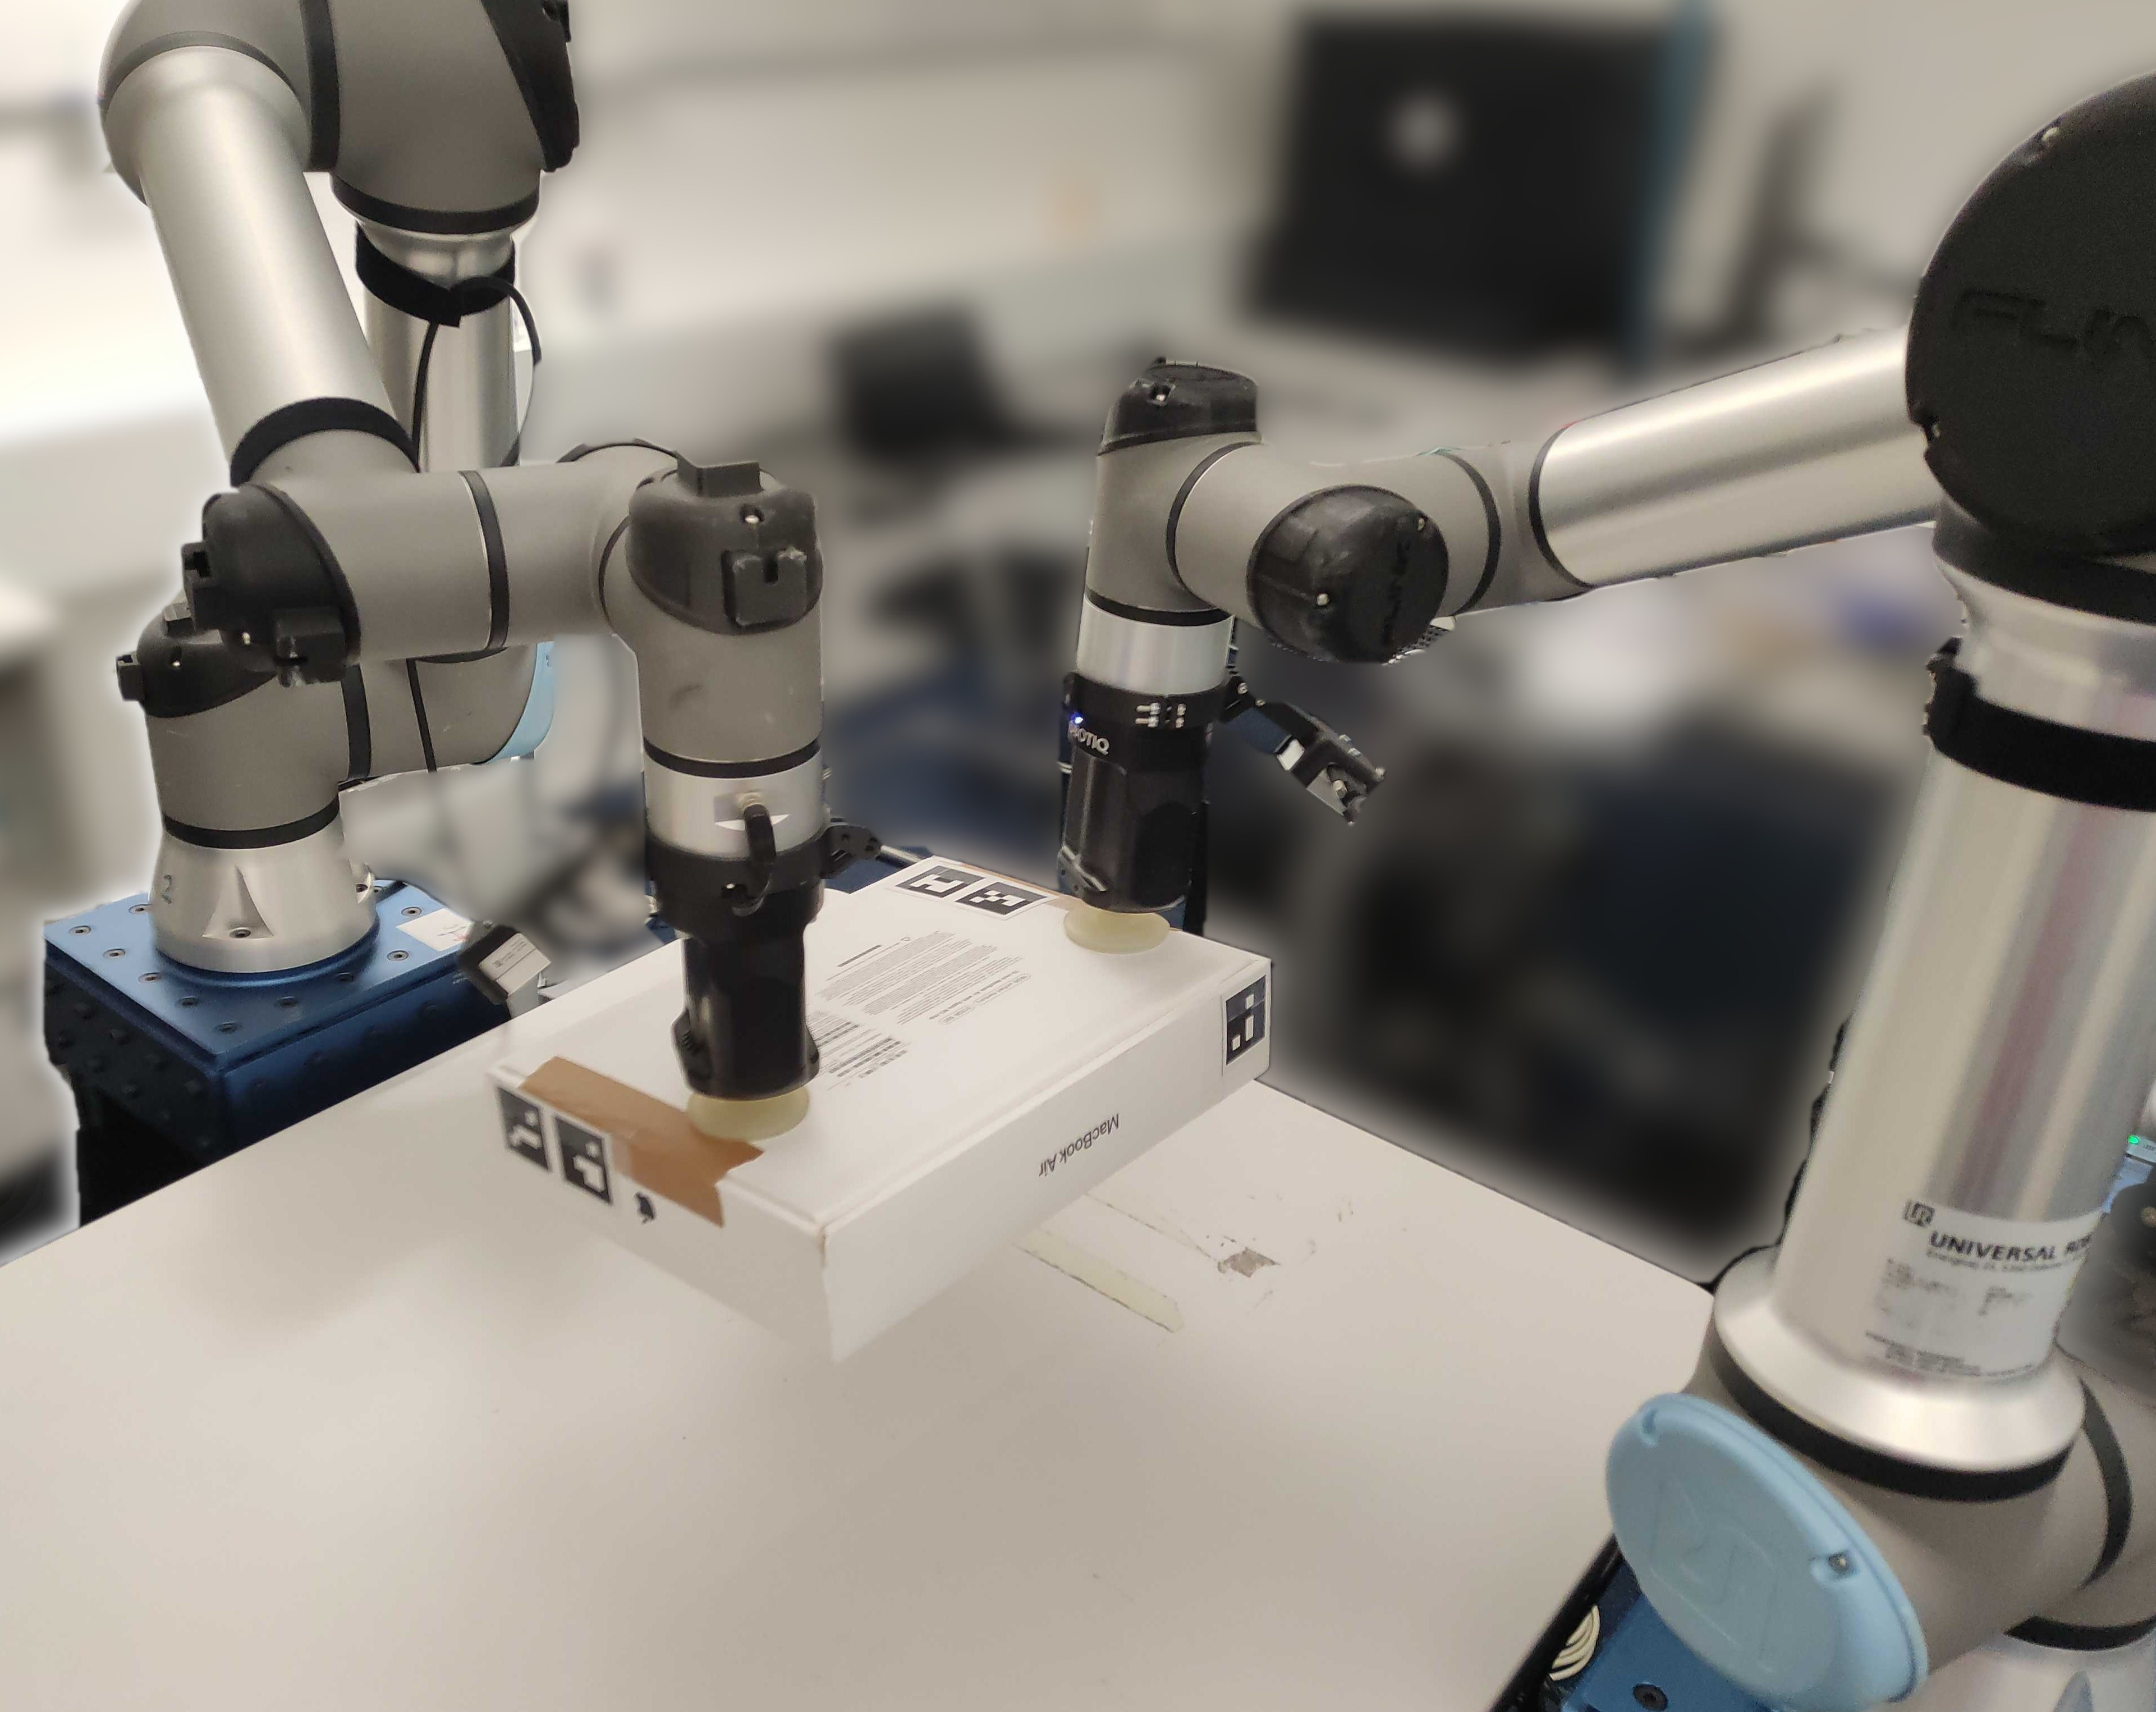
\includegraphics[width=\linewidth]{images/lift_blurred.jpg}}
        \subfigure[]{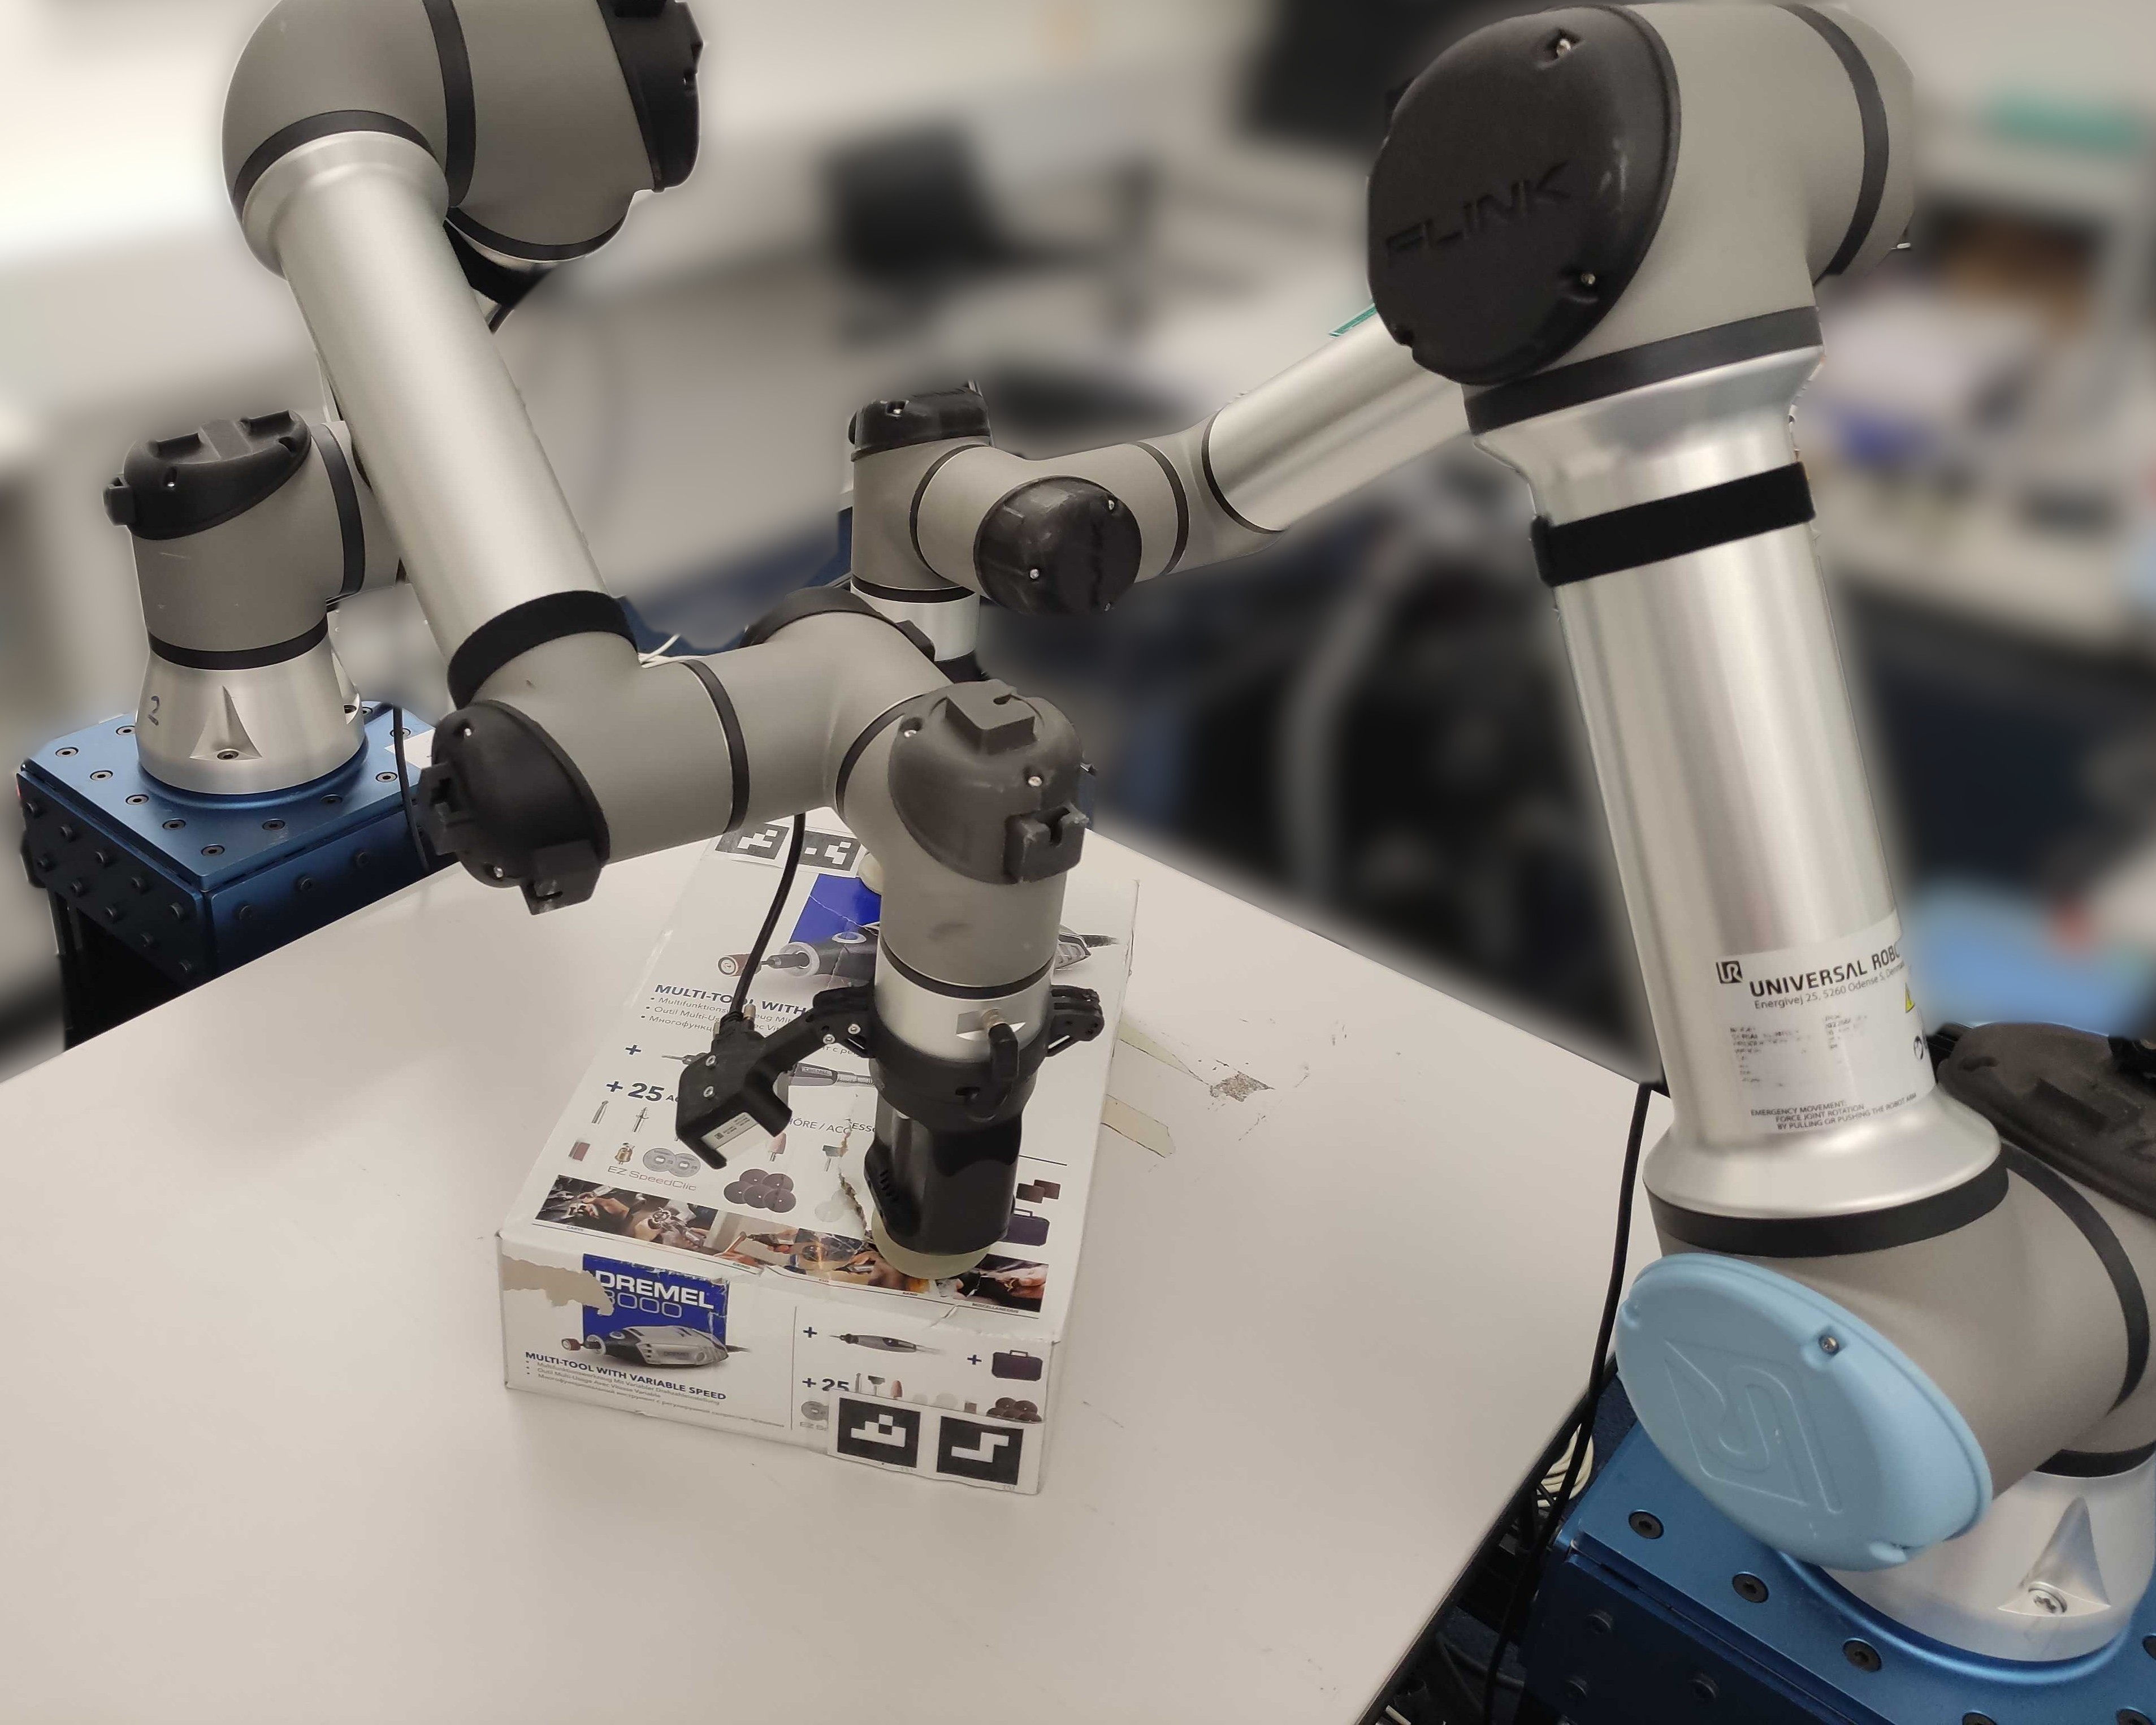
\includegraphics[width=\linewidth]{images/rot_blur.jpg}}
    \end{minipage}
    \begin{minipage}{0.35\textwidth}
        \centering
        \subfigure[]{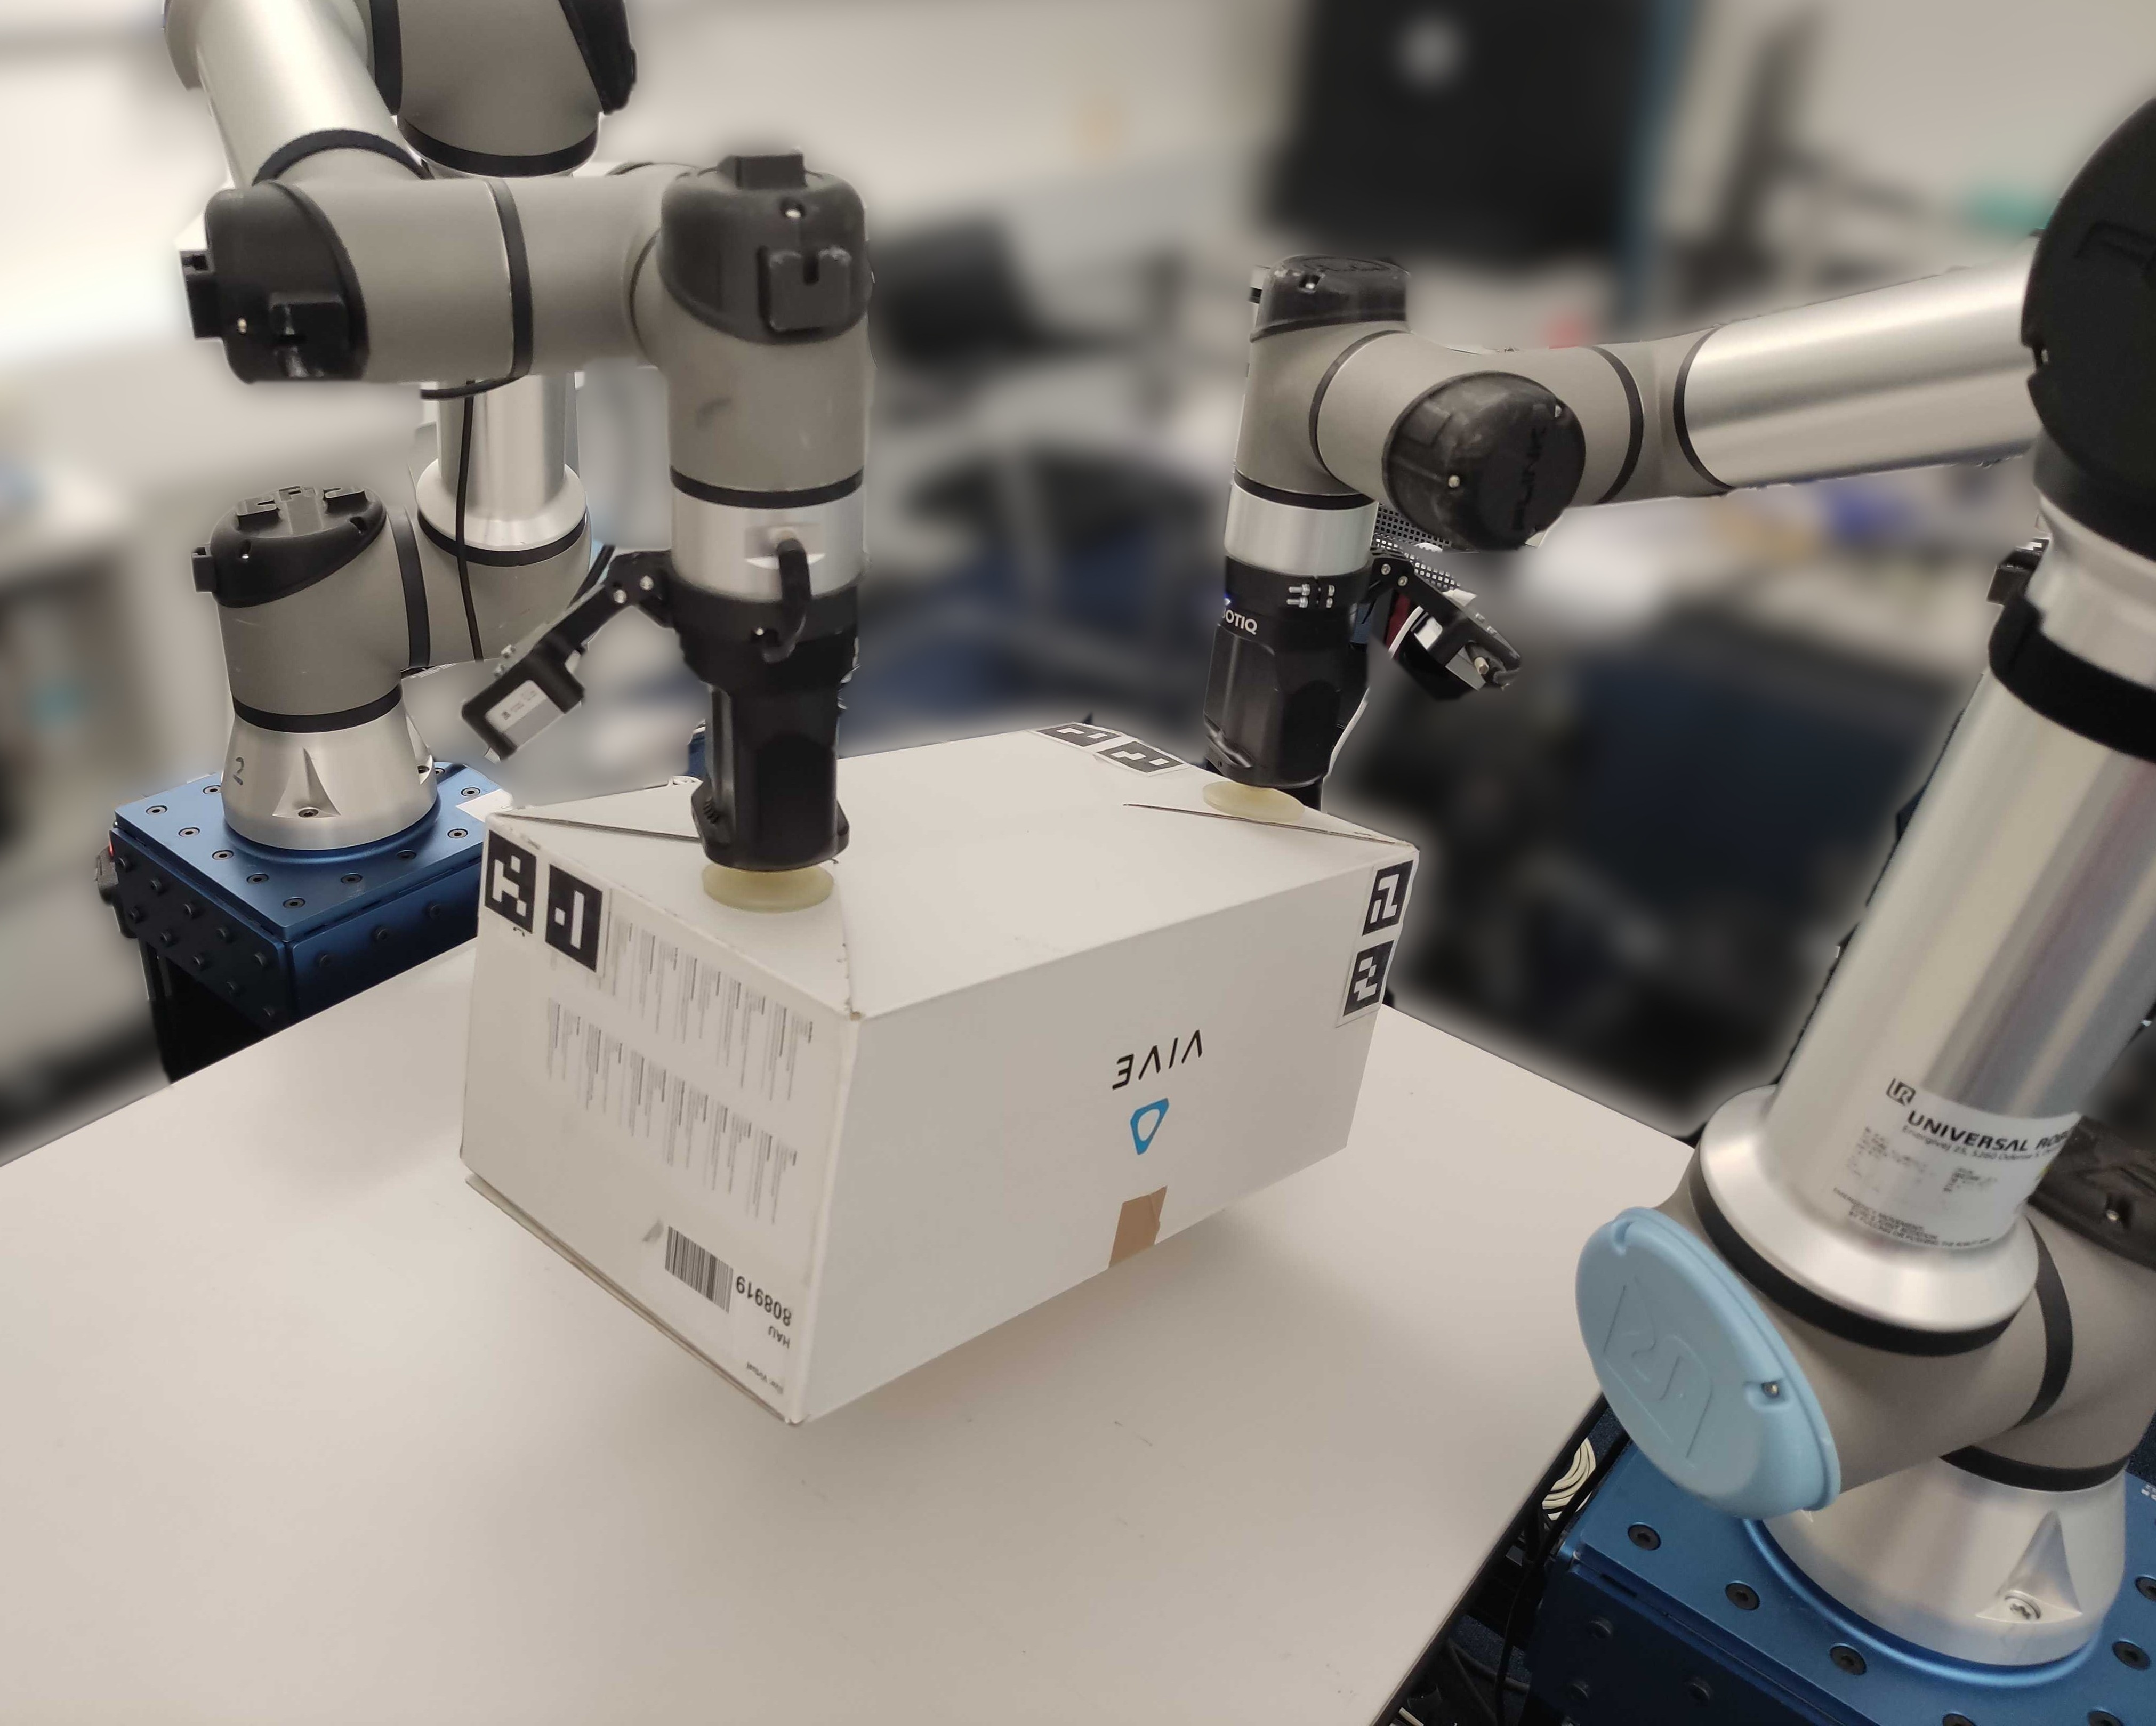
\includegraphics[width=\linewidth]{images/liftrot_blurred.jpg}}
        \subfigure[]{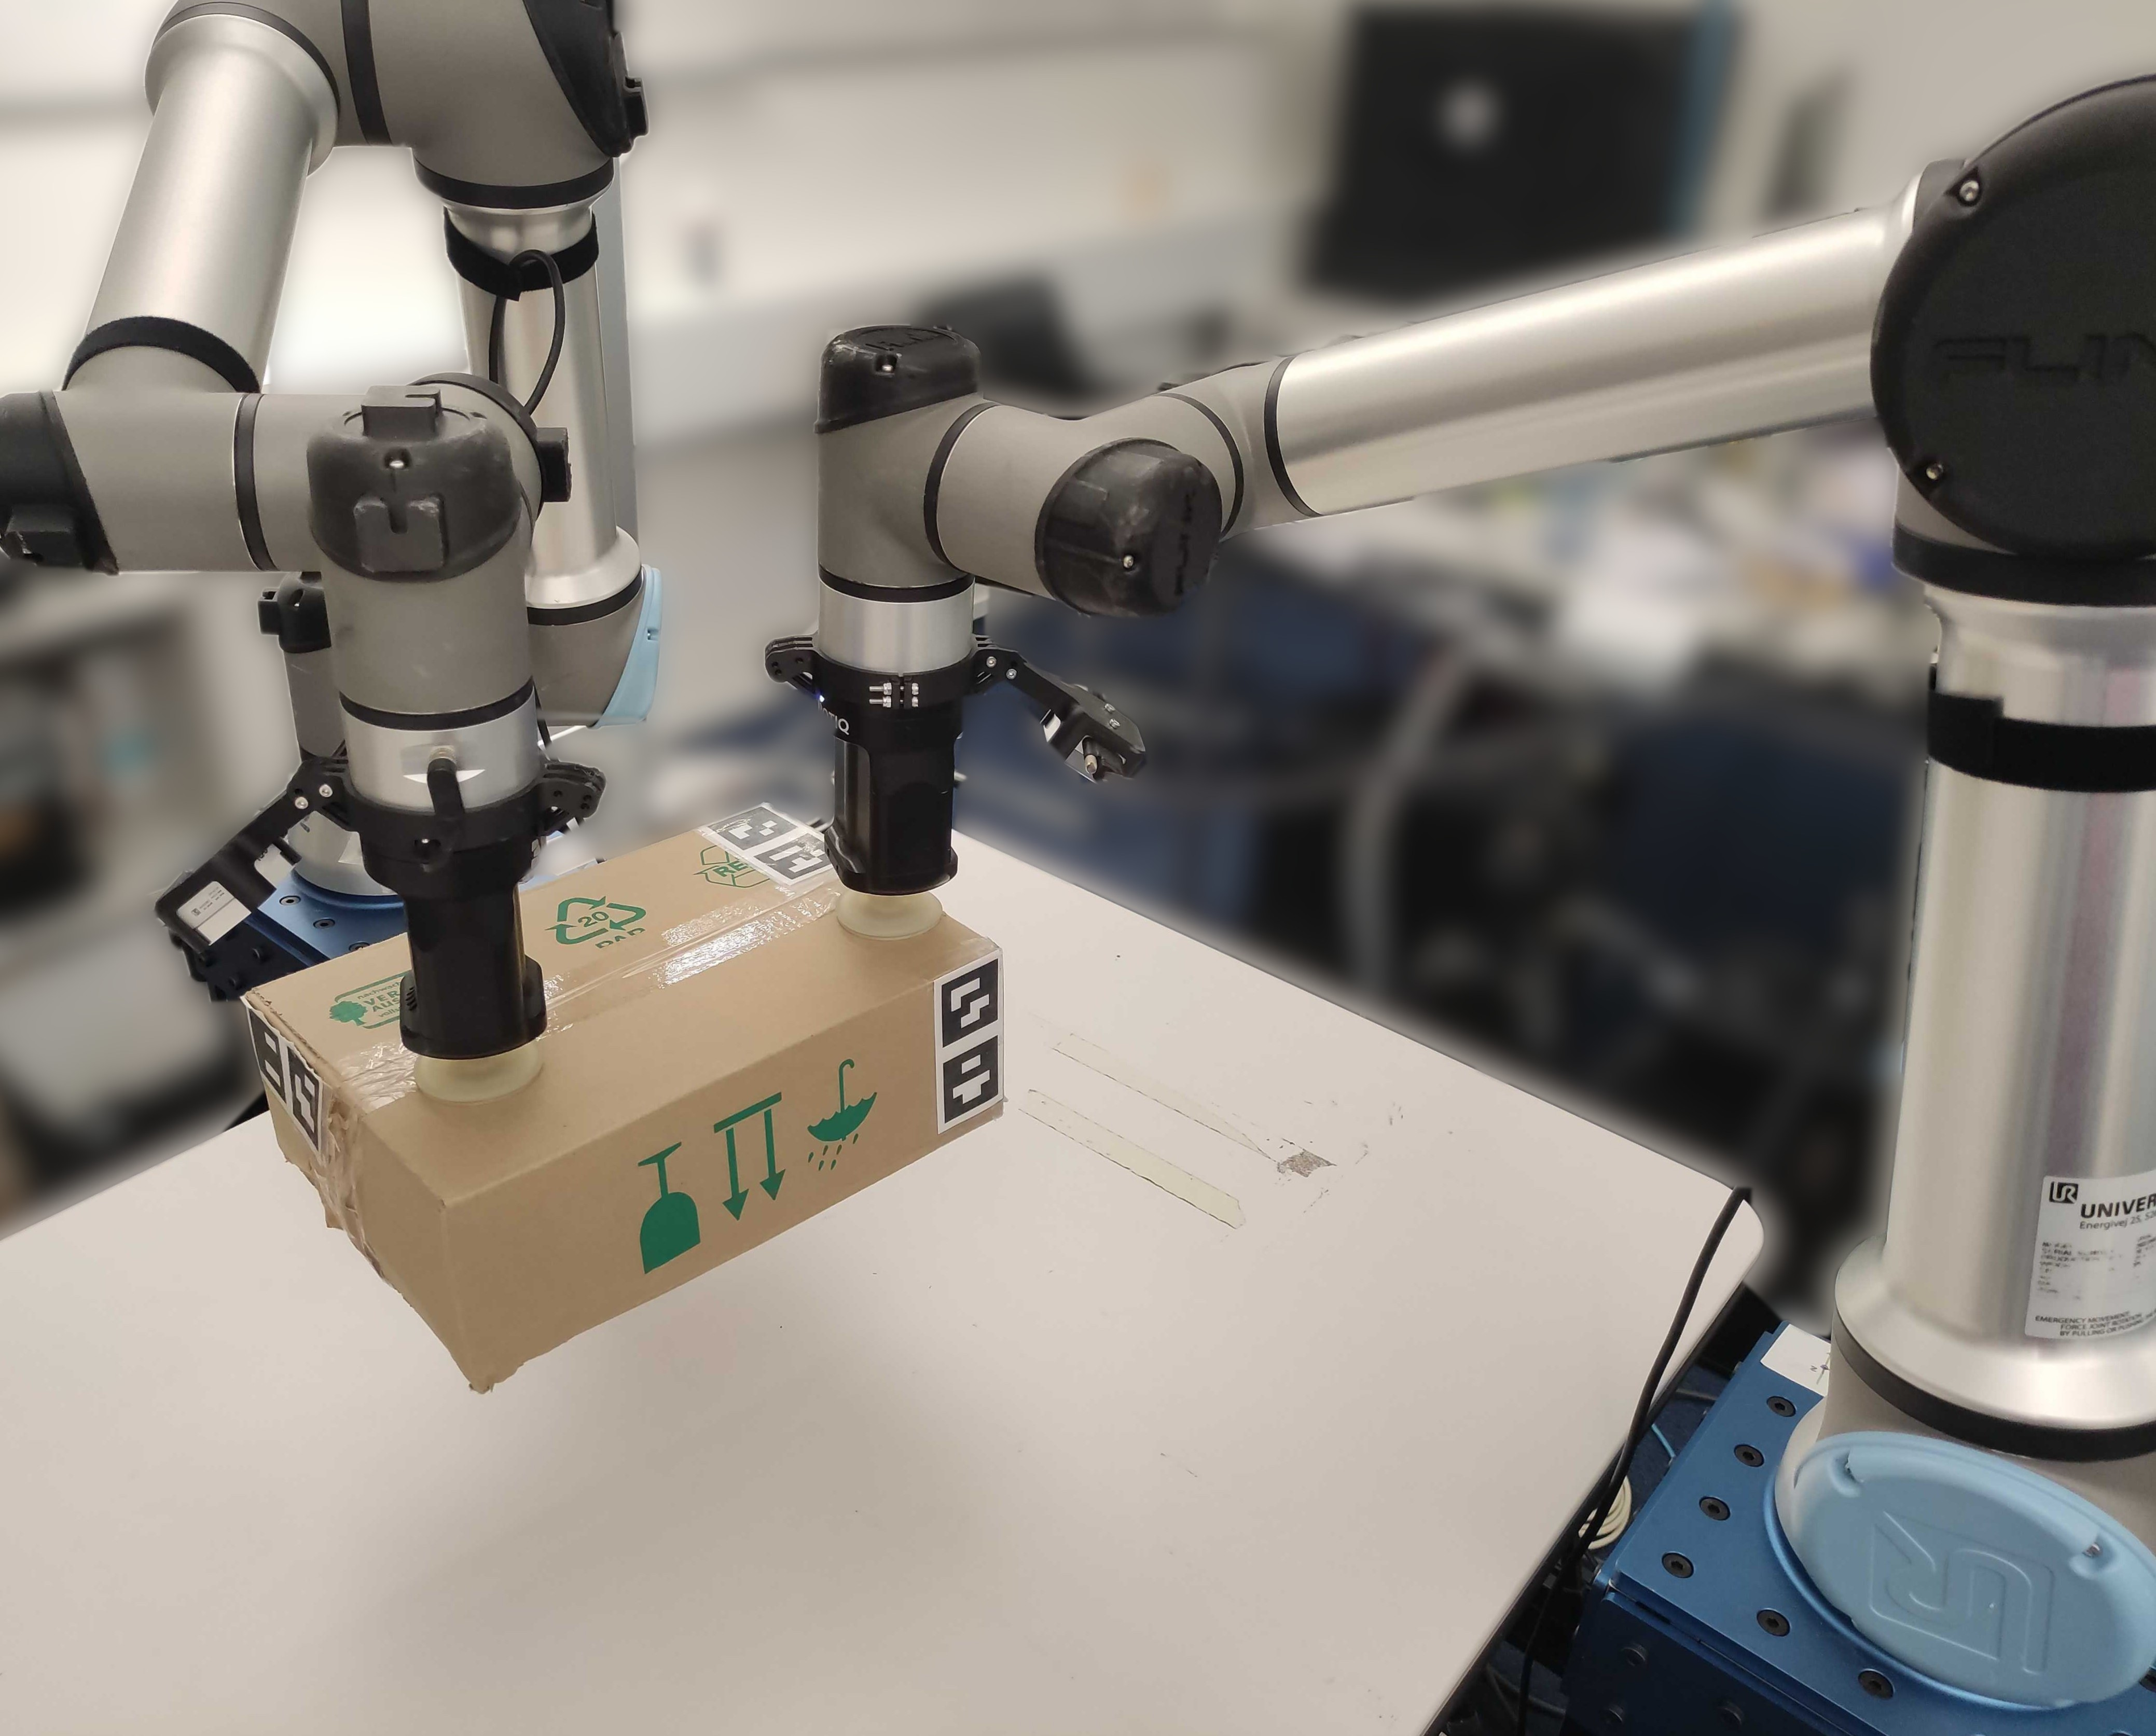
\includegraphics[width=\linewidth]{images/motion_blurred.jpg}}
    \end{minipage}
  \captionof{figure}{The dual-arm setup we used to collaboratively accomplish manipulation tasks with boxes characterized by different weights and sizes. Specifically, (a): lift, (b): rotation, (c): lift \& rotation, (d): motion.}}
    \vspace{5pt}
\makeatother

\begin{comment}
\makeatletter
\g@addto@macro\@maketitle{
  \captionsetup{type=figure}\setcounter{figure}{0}
  \centering
  \vspace{0.2cm}
    \centering
    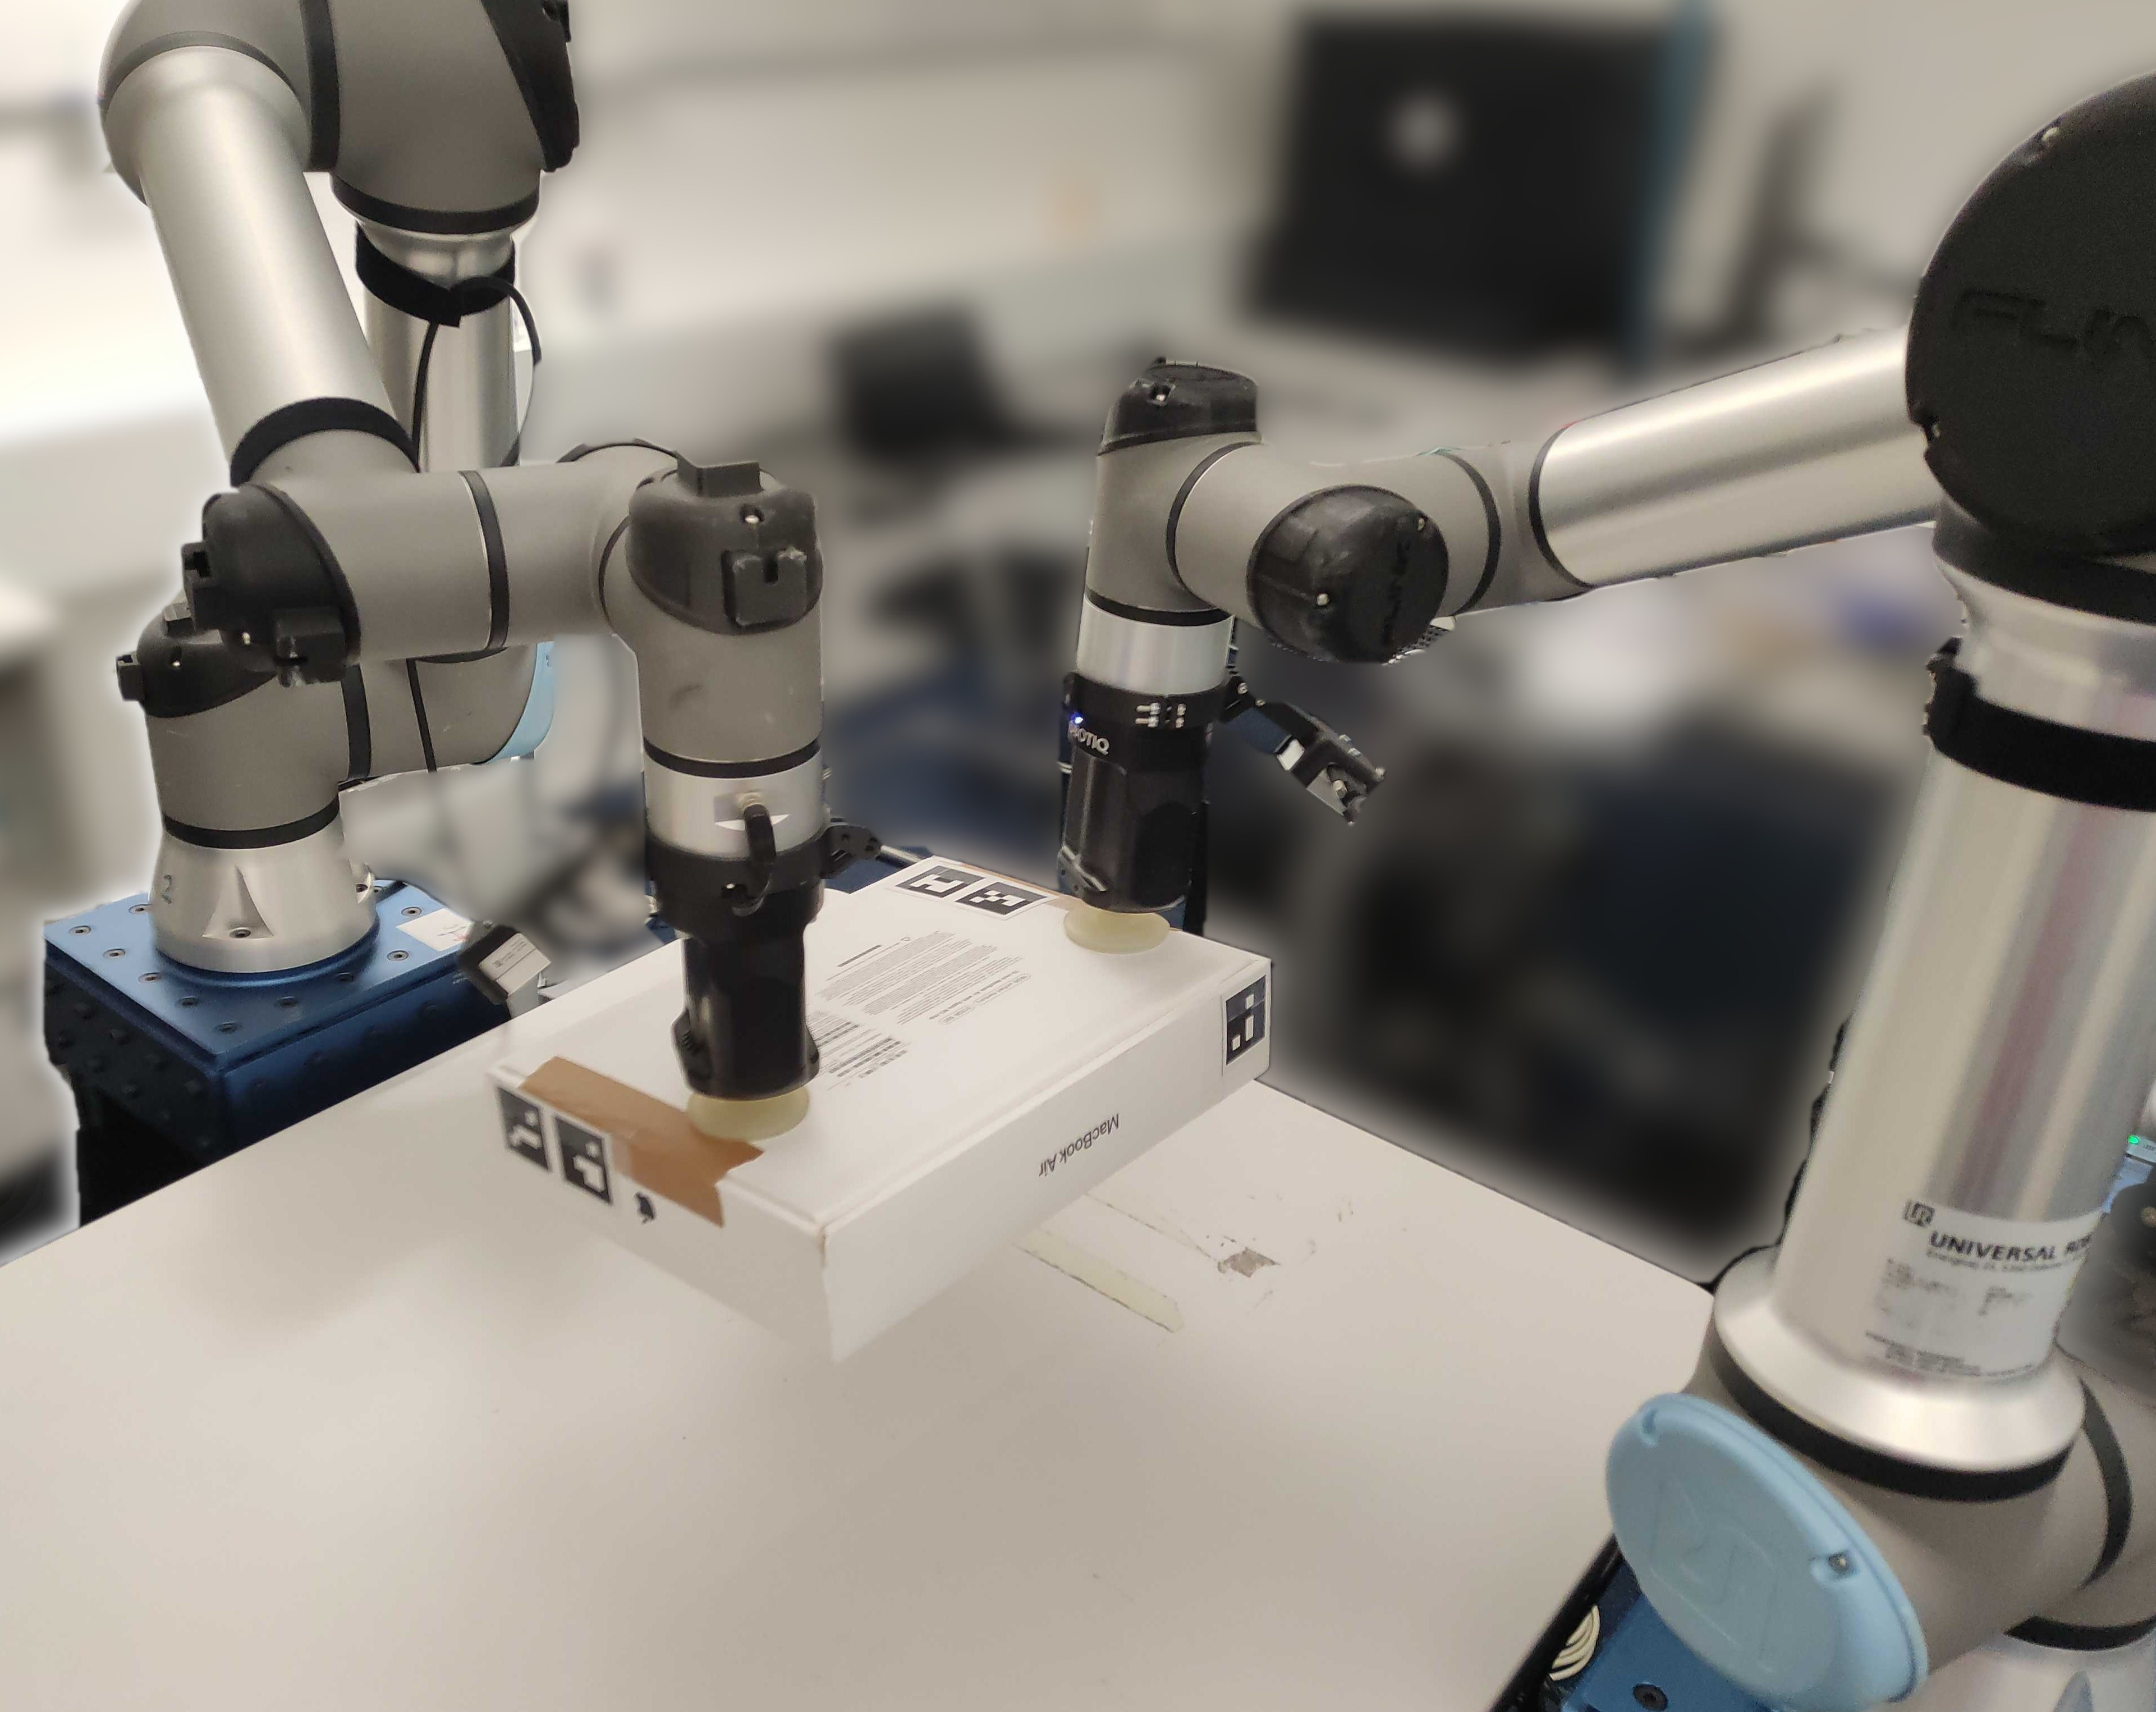
\includegraphics[width=0.22\linewidth]{images/lift_blurred.jpg}
    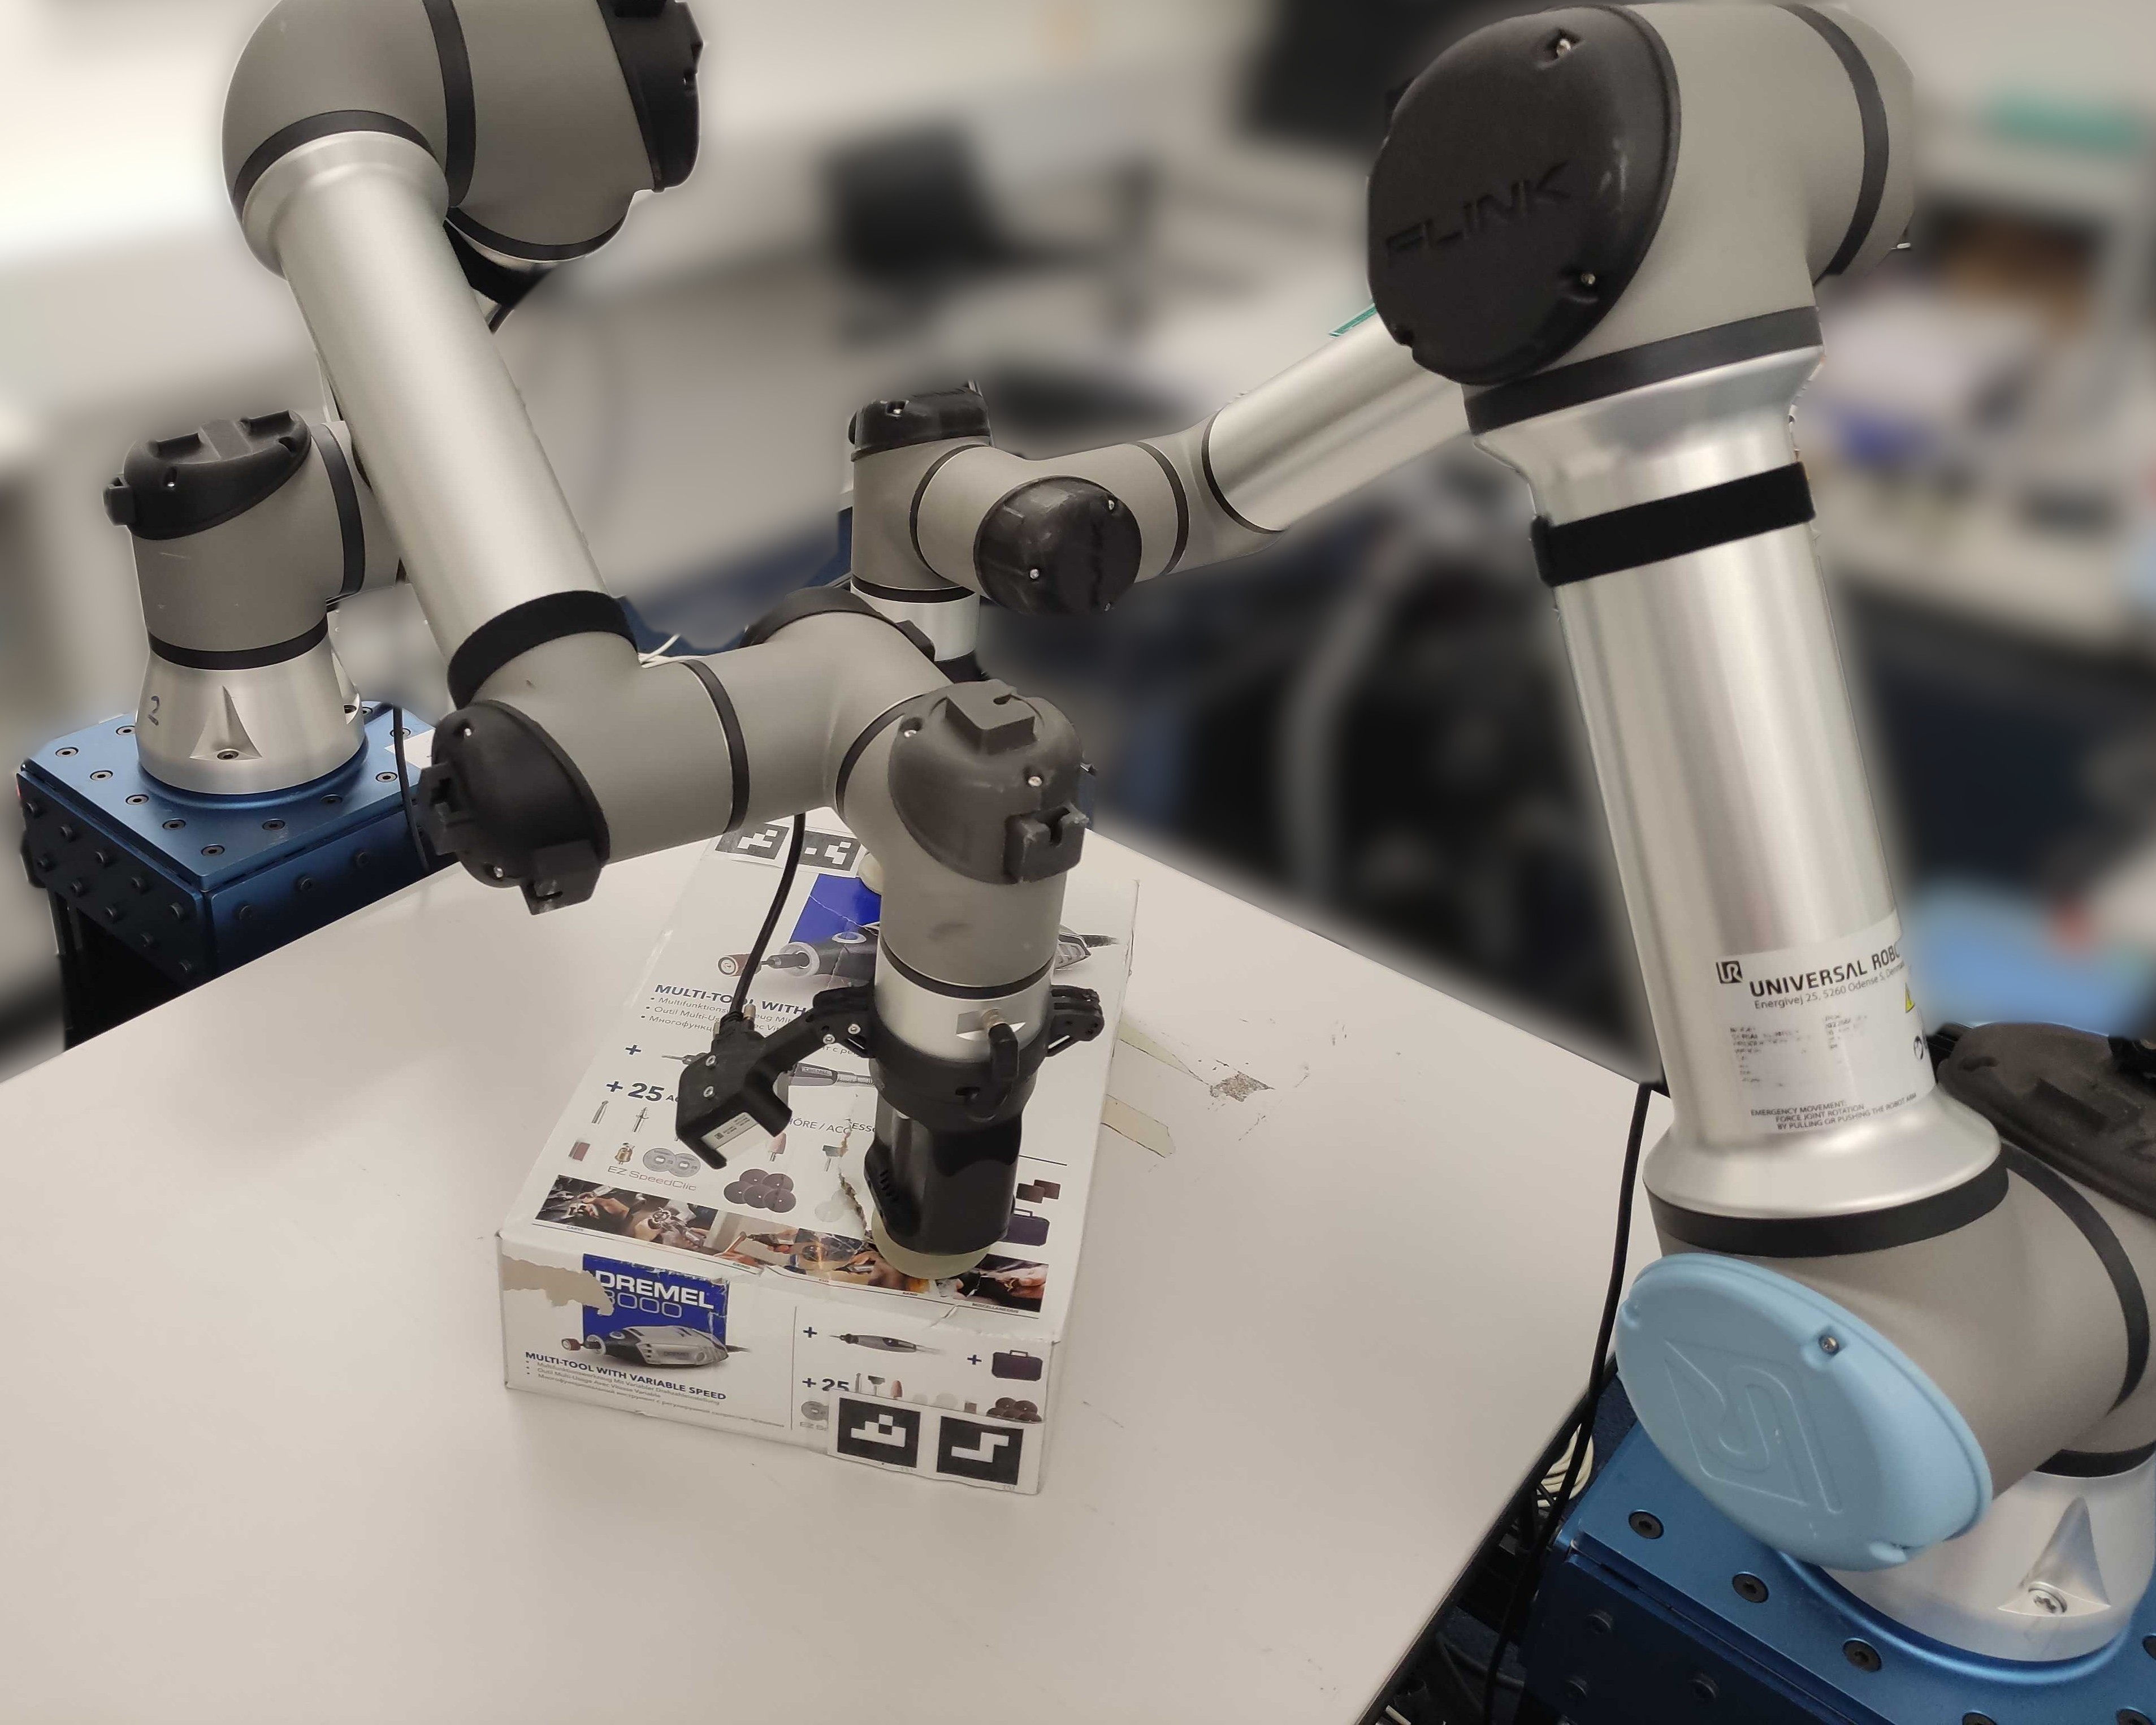
\includegraphics[width=0.22\linewidth]{images/rot_blur.jpg}
    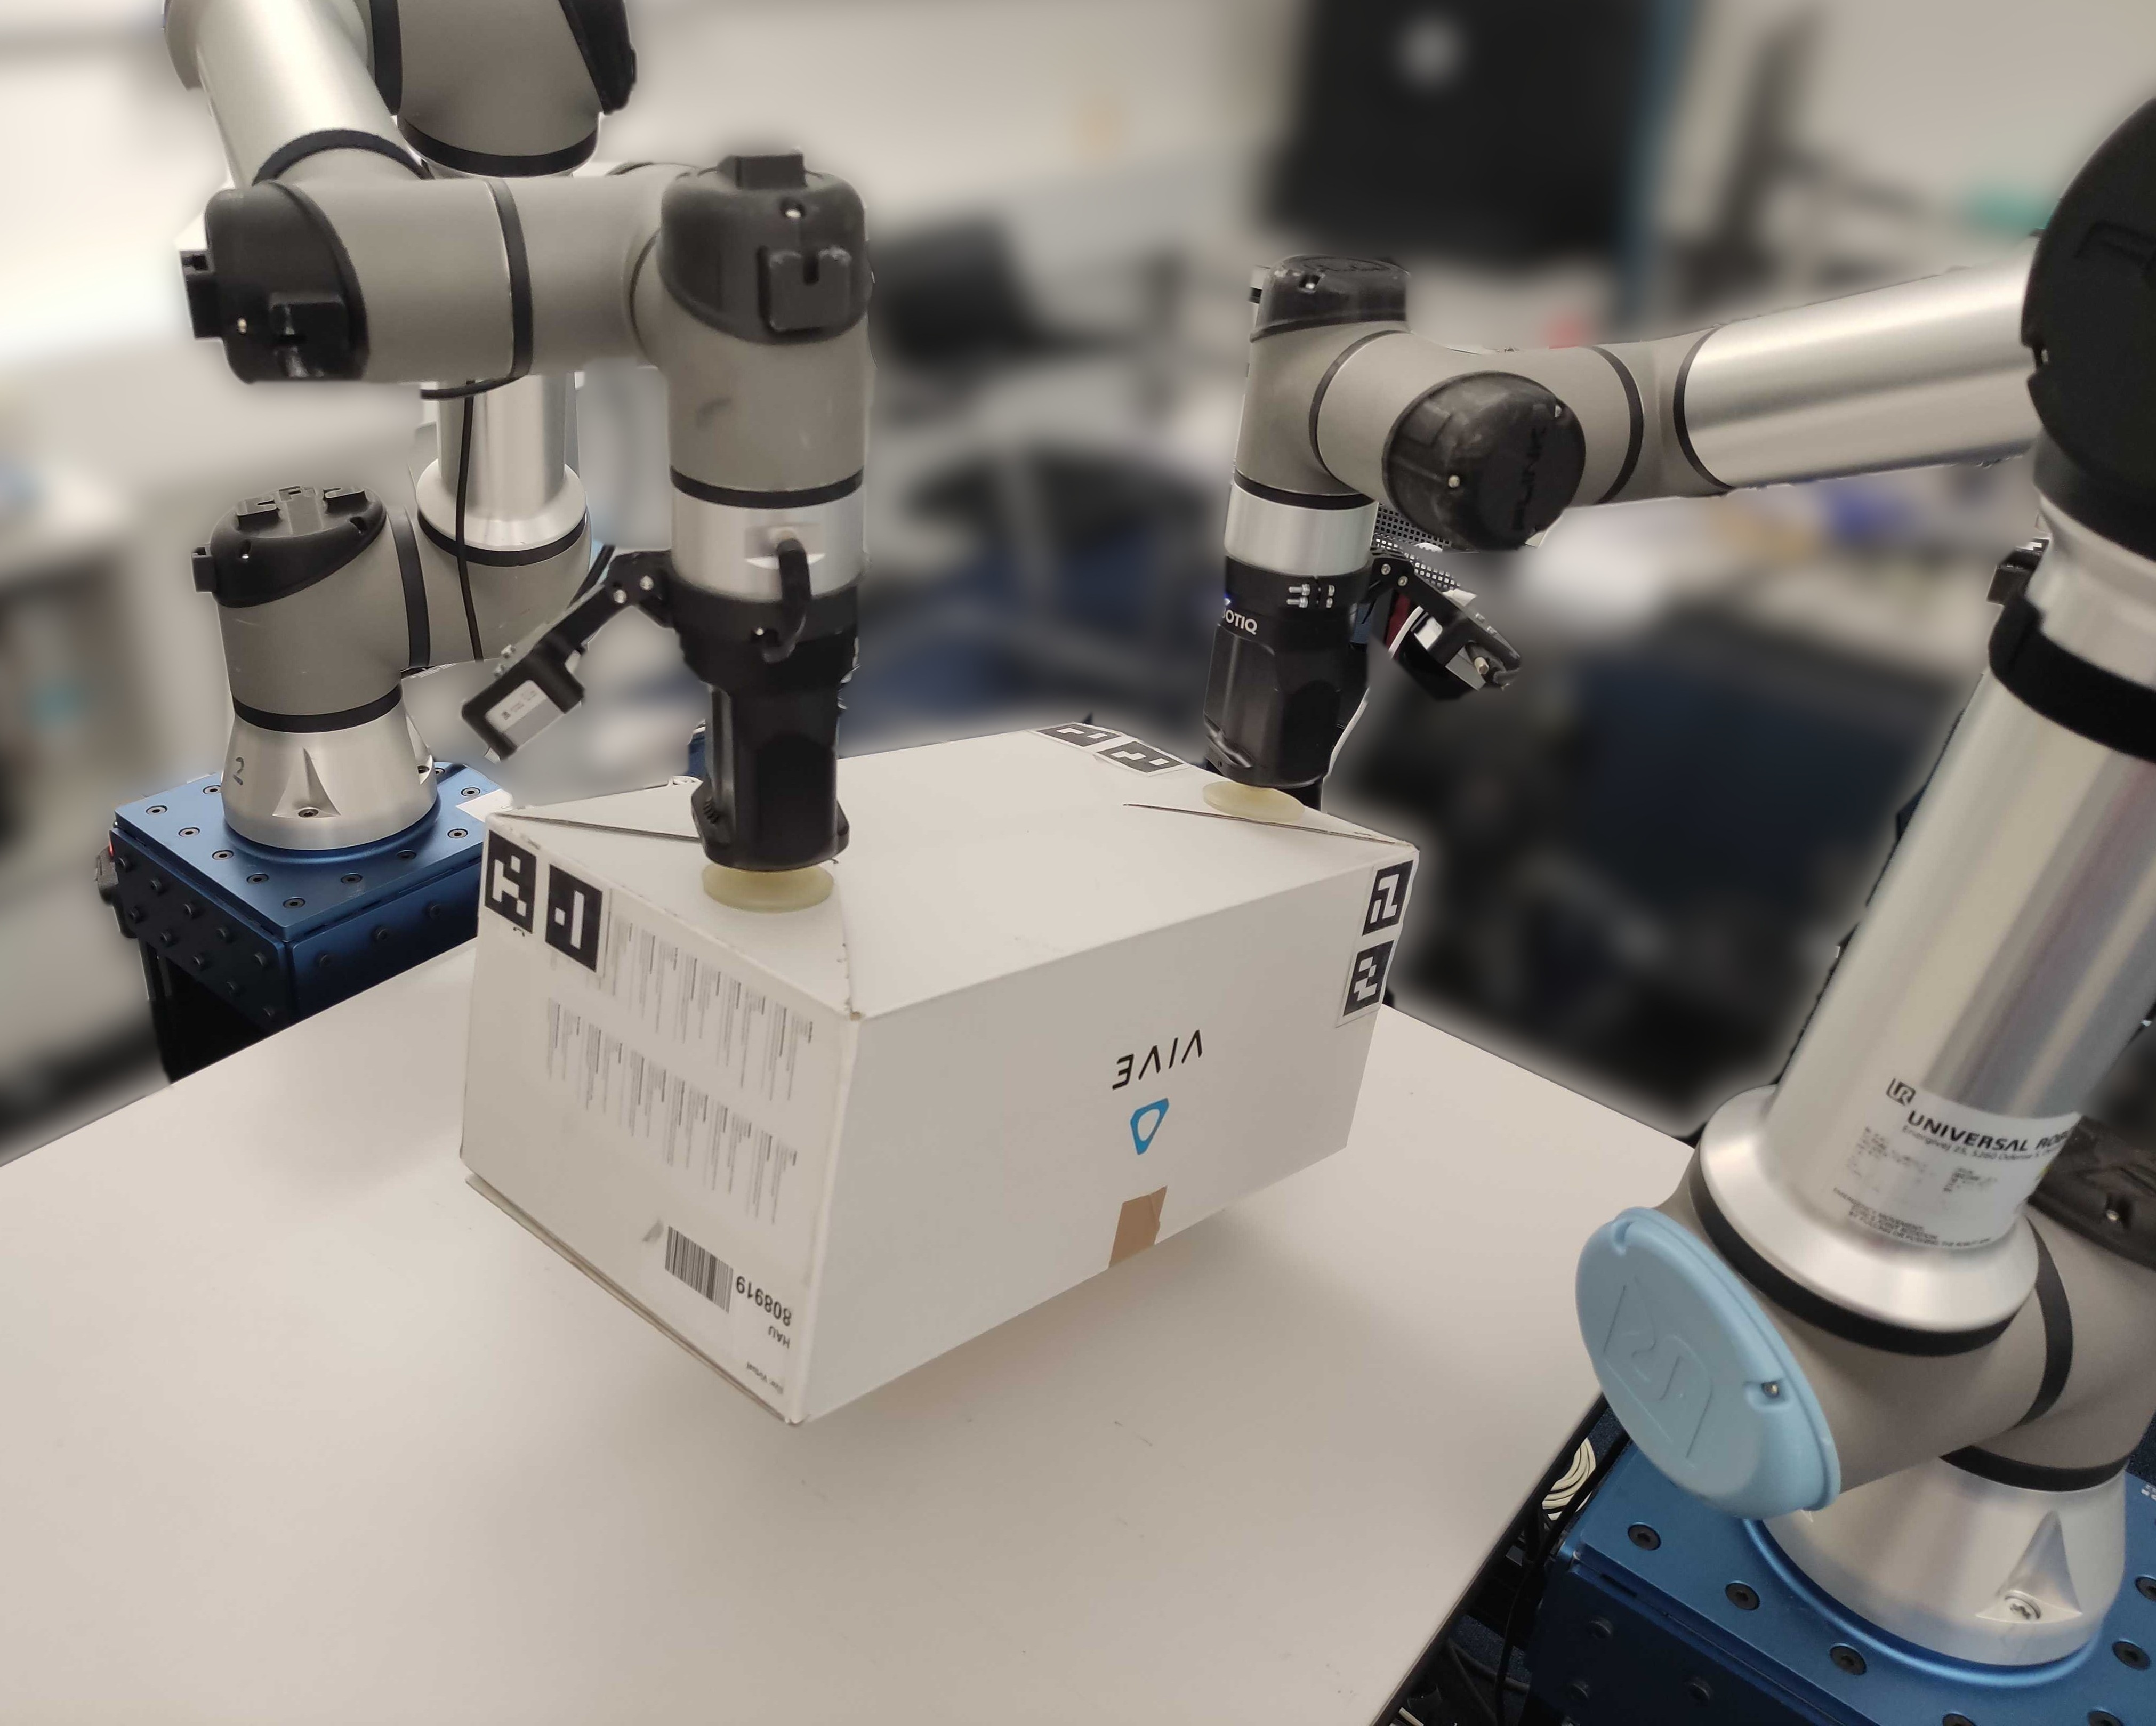
\includegraphics[width=0.22\linewidth]{images/liftrot_blurred.jpg}
    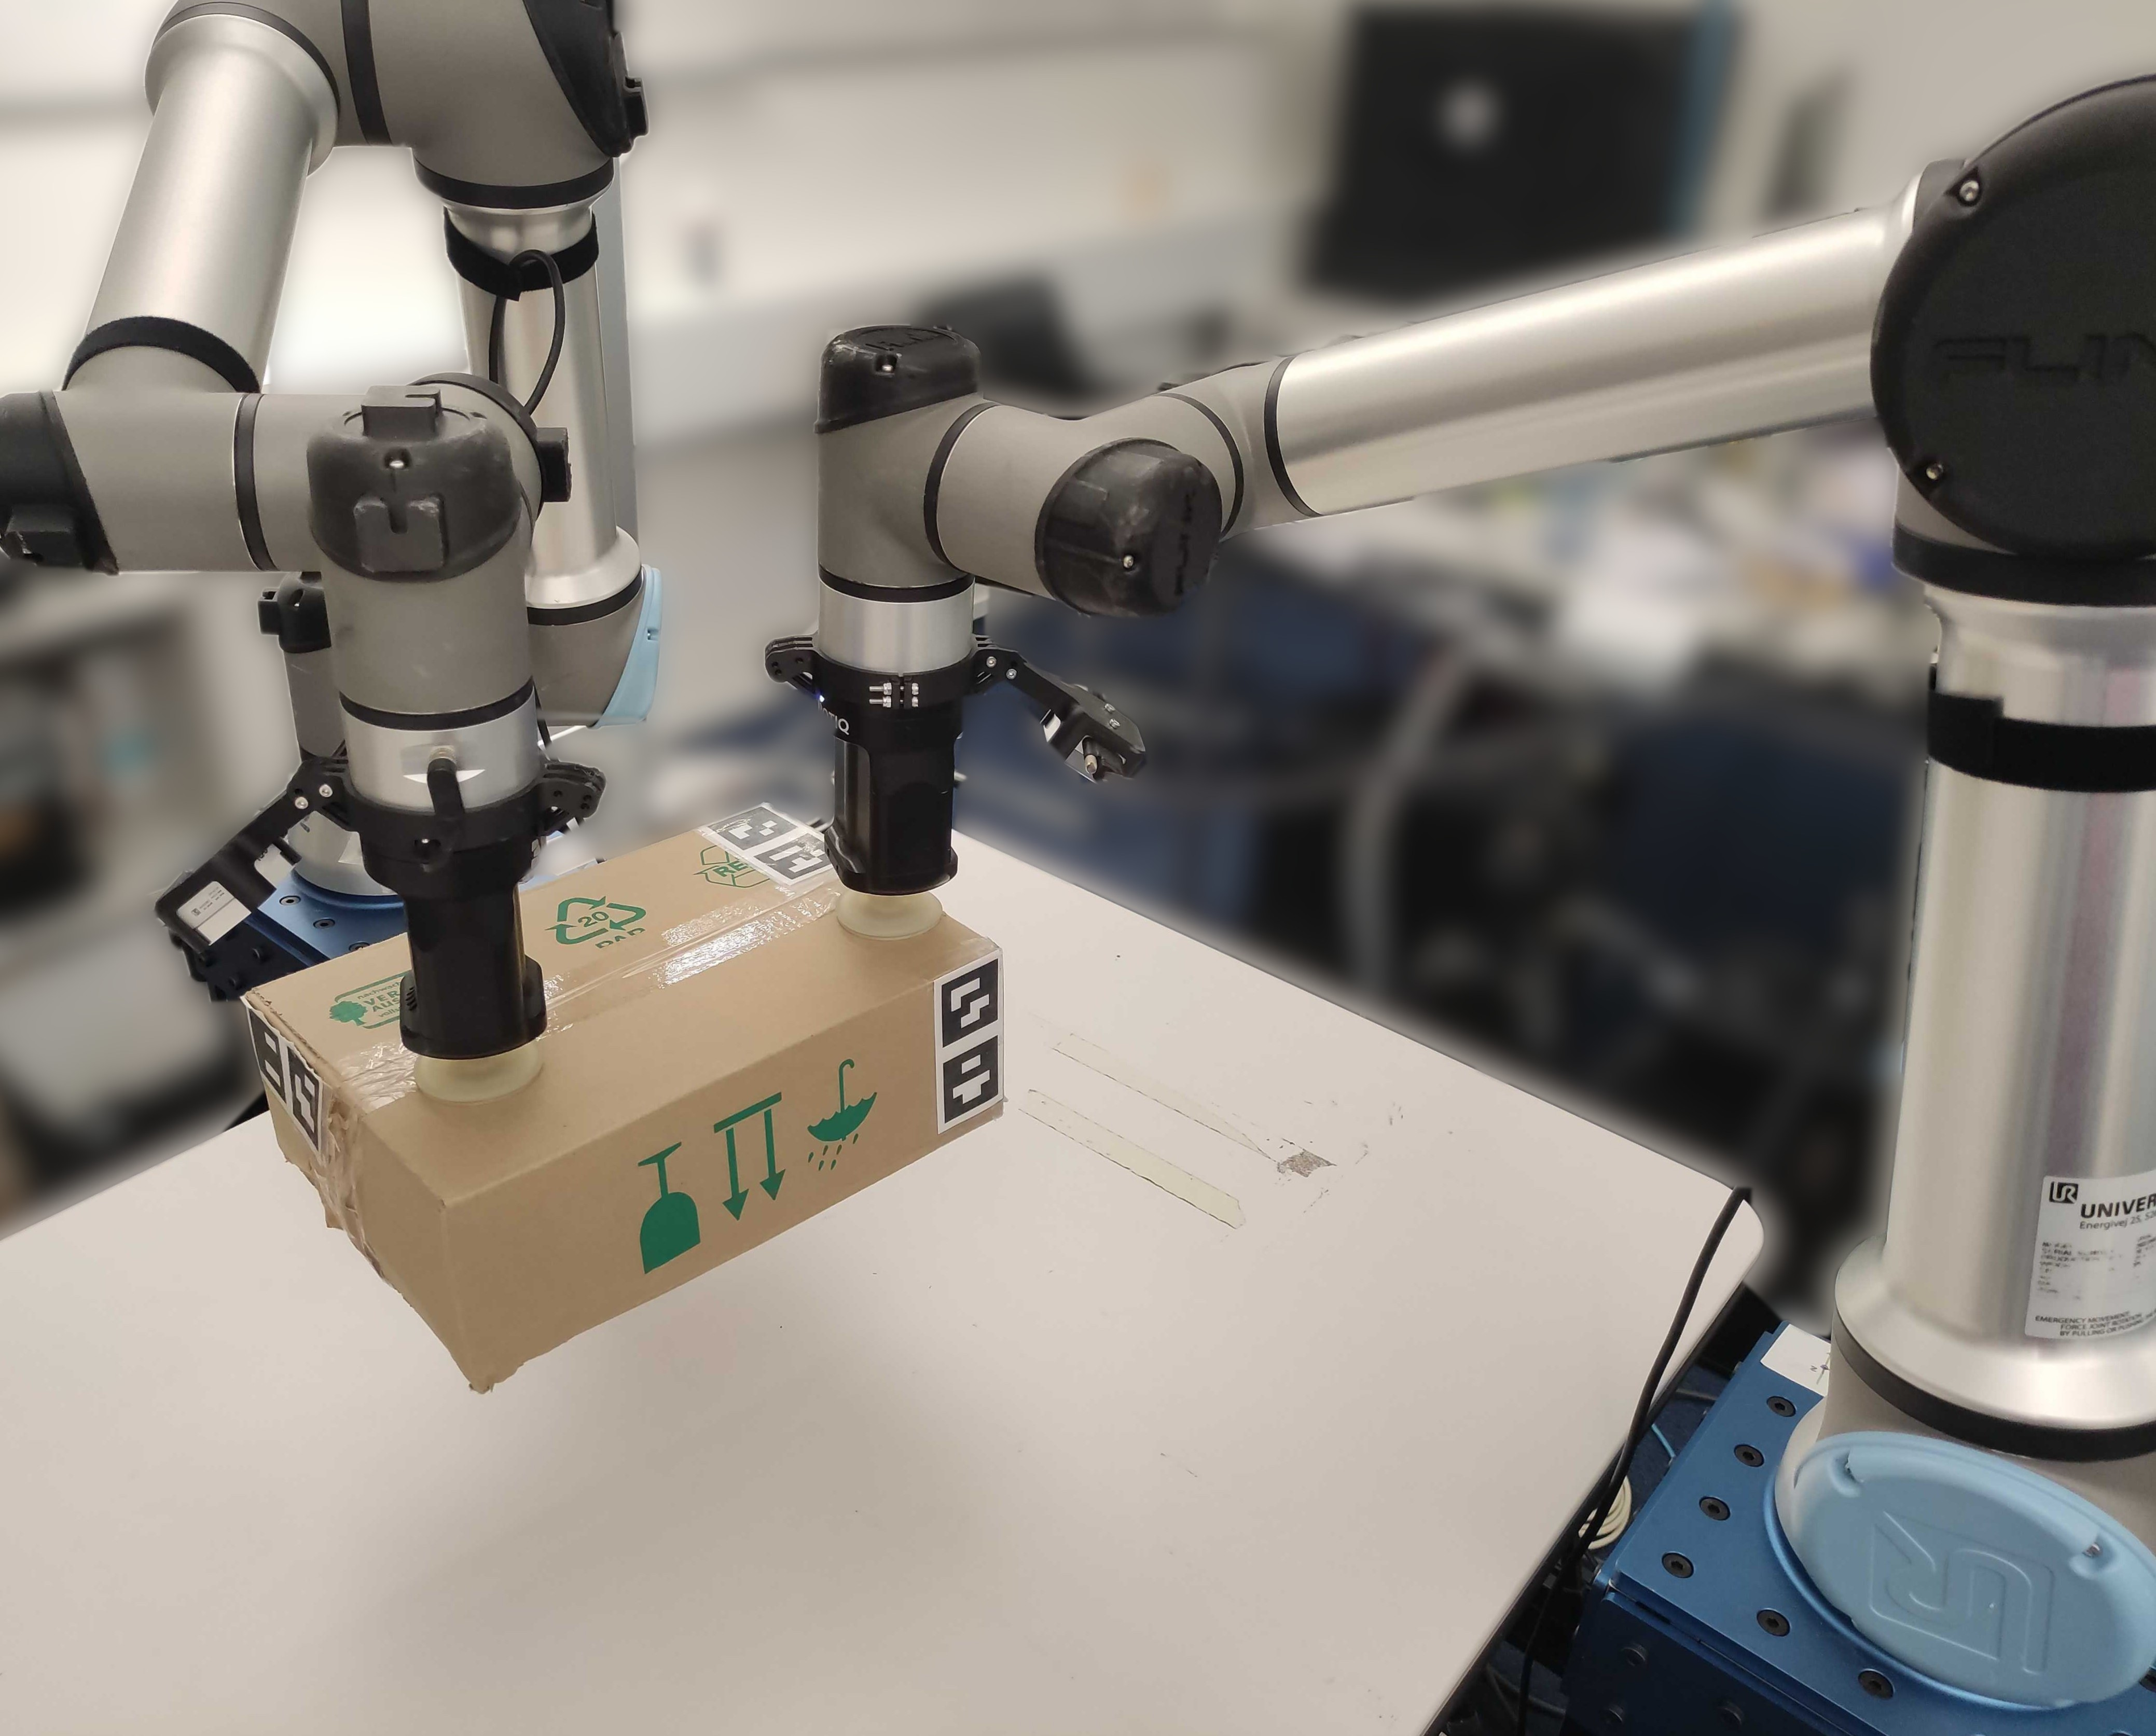
\includegraphics[width=0.22\linewidth]{images/motion_blurred.jpg}
  \captionof{figure}{A dual-arm setup to collaboratively accomplish manipulation tasks. Top left: lift, top right: rotation, bottom left: lift+rotation, bottom right: motion.}}
    \vspace{5pt}
\makeatother
\end{comment}

\maketitle
\thispagestyle{empty}
\pagestyle{empty}
%%%%%%%%%%%%%%%%%%%%%%%%%%%%%%%%%%%%%%%%%%%%%%%%%%%%%%%%%%%%%%%%%%%%%%%%%%%%%%%%
\begin{abstract}

In this work, we present a framework for dual-arm robotic systems actuated with suction cups manipulating boxes of different shapes and dimensions. We used an online reinforcement learning (RL) approach to investigate the capabilities of this setup and identify possible challenges, solutions, and applications. 
The setup integrates a perception system and visual augmentation to interpret the surroundings of the end effectors. RL allows simplifying the motion planning problem, particularly concerning collisions when the tasks are repetitive enough and the surrounding environment is well known. 
Using online RL approaches bootstrapped with human-expert demonstrations allows obtaining policies with little training time that accomplish the desired task while directly closing the sim-to-real gap. We introduced human interventions, Hindsight Experience Replay, and Residual Reinforcement Learning to improve the overall training effectiveness and efficiency. % more concrete
Considering the tasks faced more commonly in logistic centers, we trained policies that can grasp, lift, rotate and move boxes inside the workspace using two robots acting simultaneously on the objects. We validate our method through detailed real-world experiments. The code is available at \textcolor{red}{\url{https://github.com/sebastianooliani/dual-serl}}.

\end{abstract}

%%%%%%%%%%%%%%%%%%%%%%%%%%%%%%%%%%%%%%%%%%%%%%%%%%%%%%%%%%%%%%%%%%%%%%%%%%%%%%%%
\section{INTRODUCTION}

In modern industrial environments, the ability to automate complex manipulation tasks such as grasping, lifting, and positioning objects of varying shapes and sizes is crucial. Many factories use conveyor systems to transport objects for sorting, packaging, or assembly, and robotics can optimize these processes by improving speed and efficiency.

Designing an effective controller for dual-arm manipulation is a long-standing challenge. The problem was initially tackled using model-based approaches \cite{KRUGER20115}, \cite{10322775}, \cite{doi:10.1177/0278364918765952}. Those methods struggle when manipulating objects with significantly different sizes, weight distribution, and shape inconsistencies. The complexity grows even more when two robots collaborate to simultaneously manipulate an object. 
The recent successes of Reinforcement Learning and Imitation Learning approaches incentivize robotics researchers to apply them to this problem \cite{lin2023bitouchbimanualtactilemanipulation}, \cite{kataoka2022bimanualmanipulationattachmentsimtoreal}, \cite{drolet2024comparisonimitationlearningalgorithms}, \cite{luo2024precisedexterousroboticmanipulation}.
Even though manipulating a box might look trivial, there are not many solutions that actually use RL and are tested on real-world setups. Without properly designed reward functions, the agent is amenable to exploiting niches of the environment that create inappropriate, non-robust, and potentially unsafe solutions.

In this work, we compare the performance of learning-based policies for dual-arm manipulation of boxes to traditional model-based approaches. 
Policies for similar tasks were extensively studied for single-arm and dual-arm systems in simulation \cite{nair2018overcomingexplorationreinforcementlearning}, \cite{huang2024mrhermodelbasedrelayhindsight}, \cite{makarova2025contherhumanlikecontextualrobot}, \cite{Horv_th_2024}, but only few real-world implementations are available \cite{wang2025oneshotdualarmimitationlearning}, \cite{mu2025robotwindualarmrobotbenchmark}, \cite{wang2025learningdualarmcoordinationgrasping}. To the best of our knowledge, no previous work trained an online RL policy for a dual-arm setup actuated with suction cups.

This work is strongly based on \cite{sutter2025comparisonvisualrepresentationsrealworld}. This study focuses on determining how different encoders can be used in a reinforcement learning framework to interpret the spatial environment in the local surroundings of a robot arm. 
It is the first work to train a reinforcement learning policy for a suction gripper using point cloud inputs with real-world data. 
In particular, it shows that 3D voxel grid representations are particularly beneficial for spatial perception, outperforming other image-based policies. 
As a result, point cloud is directly used in this work as the main visual backbone, without comparing its performance with other image-based encoders. 
The whole framework is also based on SERL \cite{luo2024serlsoftwaresuitesampleefficient}, a software suite for robotic RL with sample-efficient off-policy algorithms. It provides a set of useful packages and libraries to control and train RL agents. In particular, training is performed online using several state-of-the-art algorithms such as Soft Actor Critic (SAC) \cite{haarnoja2018softactorcriticoffpolicymaximum}, and Reinforcement Learning with Prior Data (RLPD) \cite{ball2023efficientonlinereinforcementlearning}, and can be bootstrapped with human-expert demonstration. 
% One of the main advantages of SERL is that it can successfully train a policy and deploy it on a real robot with little training time (from 30 minutes to 2 hours, depending on the CPU).
% SERL is particularly efficient because it takes advantage of both offline and online RL, i.e. initializing the replay buffer with human-expert demonstrations and then running the training online \cite{song2023hybridrlusingoffline}. 

To the best of our knowledge, our system is the first to (1) achieve dual-arm coordination with point cloud inputs using RL in real-world settings, (2) train policies for dual-arm systems using a limited number of human-expert demonstrations and within a relatively short time, and (3) train dual-arm manipulation policies actuated with suction grippers using Hindsight Experience Replay (HER) \cite{andrychowicz2018hindsightexperiencereplay} and Residual RL (RRL) \cite{johannink2018residualreinforcementlearningrobot} while relying on data collected solely in the real-world. 

\section{RELATED WORK} % TODO: this part needs to be a bit longer. mention any possible approach to dual arm manipulation and real world rl. look if someone implements her the real world

The work in \cite{10322775} proposes and validates a model predictive control (MPC) algorithm for online time-optimal trajectory planning of cooperative robotic manipulators. %, utilizing velocity constraints and tangent-separating planes for collision avoidance. 
In particular, it shows that using two robot arms in a tight, shared workspace leads to an improvement in cycle times compared to deploying a single robot to execute the same tasks. 
% This improvement enables a more efficient robot operation.

The work in \cite{lin2023bitouchbimanualtactilemanipulation} offers an overview and comparison of the main state-of-the-art algorithms for Imitation Learning in robotic manipulation. 
A successful approach based on Imitation Learning for bimanual manipulation is presented in \cite{zhao2023learningfinegrainedbimanualmanipulation}. It trains and deploys policies on low-cost robots, thanks to its Action-Chucking Transformer (ACT). The work in \cite{wang2025oneshotdualarmimitationlearning} introduced an Imitation Learning based method to deploy policies in dual-arm setups using a single demonstration.
% According to it, Generative Adversarial Imitation Learning (GAIL), Diffusion Policy, and ACT are viable options for bimanual manipulation.

The works presented in \cite{huang2024mrhermodelbasedrelayhindsight}, \cite{makarova2025contherhumanlikecontextualrobot}, and \cite{Horv_th_2024} showed in simulation that the combination of RL with HER or its modification can effectively boost the performance of common manipulation tasks, like pushing, pick \& place, and path following. 
As an example of a real-world implementation of HER, the work in \cite{wang2025maernavbidirectionalmotionlearning} trained an RL policy that integrated HER in simulation and implemented it in a real-world setting for robot navigation.

The work in \cite{wang2025learningdualarmcoordinationgrasping} deployed a dual-arm RL policy in the real-world for grasping large-sized objects. The policy was trained in simulation using a CNN-based Proximal Policy Optimization (PPO) algorithm \cite{schulman2017proximalpolicyoptimizationalgorithms} and used RGB images as visual backbone.

The work most similar to ours is \cite{luo2024precisedexterousroboticmanipulation}. It presents the first robotic system which achieves dual-arm coordination with image inputs using Reinforcement Learning in real-world settings. 
In particular, it bootstraps the training using human-expert demonstration and introduces a human-in-the-loop (HIL) feedback approach during the training. 
%Easily speaking, this means that every time the SpaceMouses are pressed, the actions saved in the transitions are the ones performed by the human operator, which should provide corrective actions. 
This work outperforms Imitation Learning algorithm methods that are trained on the same amount of human data to perform dual-arm tasks like object handover and collaborative assembly.

\section{BACKGROUND}
We formulate the general RL task as a partially observable Markov decision process (POMDP) \cite{cbf00562-4ec1-30aa-96c9-a7b516c45b2b}, \cite{KAELBLING199899}. A POMDP can be described as a tuple $(\mathcal{O}, \mathcal{A}, p, r, \gamma)$, where $\mathcal{O}$ is the observation space, $\mathcal{A}$ is the action space, $p$ is the unknown and potentially stochastic transition probability that depends on the system dynamics, $r:\mathcal{O} \times \mathcal{A} \rightarrow \mathbb{R}$ is the reward function that maps the current observation and action to reward $r_t=r(o_t,a_t)$ and $\gamma$ is the discount factor. 
The goal is to find an optimal policy $\pi(a_t|o_t)$, that maximizes the expected cumulative return given by $\mathbb{E}_\pi\sum_{t=0}^\infty\gamma^tr_t$.

\subsection{Soft Actor Critic (SAC)}
SAC \cite{haarnoja2018softactorcriticoffpolicymaximum} is an RL algorithm for continuous control tasks that optimizes a stochastic policy $\pi_{\theta}$ by maximazing both policy entropy \cite{10.5555/1620270.1620297} and expected reward via the state-action value function $Q_\theta$, encouraging exploration. Since SAC cannot effectively handle high-dimensional observation spaces like images or pointcloud data, we use this state-of-the-art off-policy algorithm as a baseline for comparison with more advanced policies.

\subsection{Reinforcement Learning with Prior Data (RLPD)}
RLPD \cite{ball2023efficientonlinereinforcementlearning} is an RL algorithm based on SAC, which aims to make real-world RL efficient. Key modifications to SAC include: (1) high update-to-data ratio during training, (2) symmetric sampling of prior and on-policy data, and (3) layer-norm regularization during training. While this method can train from scratch, it is often useful to bootstrap learning using prior data, for example demonstrations.

\subsection{Data-Regularized Q (DRQ)}
DRQ \cite{kostrikov2021imageaugmentationneedregularizing} is a simple data augmentation technique that can be applied to any standard model-free RL algorithm. In SERL, it is built on RLPD \cite{ball2023efficientonlinereinforcementlearning}. With this approach, we are able to find an optimal policy for a POMDP $(\mathcal{O}, \mathcal{A}, p, r, \gamma)$, using either RGB images, depth images or a voxel grid as additional observation inputs. 
% These high-dimensional observation spaces and their corresponding encoder will be further described in the upcoming section.

\section{METHODOLOGY}

In this section, we describe the different methods we exploited to train RL policies that could be effectively deployed on dual-arm systems. Considering the tasks we want to achieve and starting from a simple model-based controller, we tackled the main challenges caused by the high dimensionality of the problem and the need for policies that require reasonable training time to converge.

\subsection{Creating a benchmark for dual-arm manipulation}

\begin{figure}[t]
    \centering    
    \subfigure[]{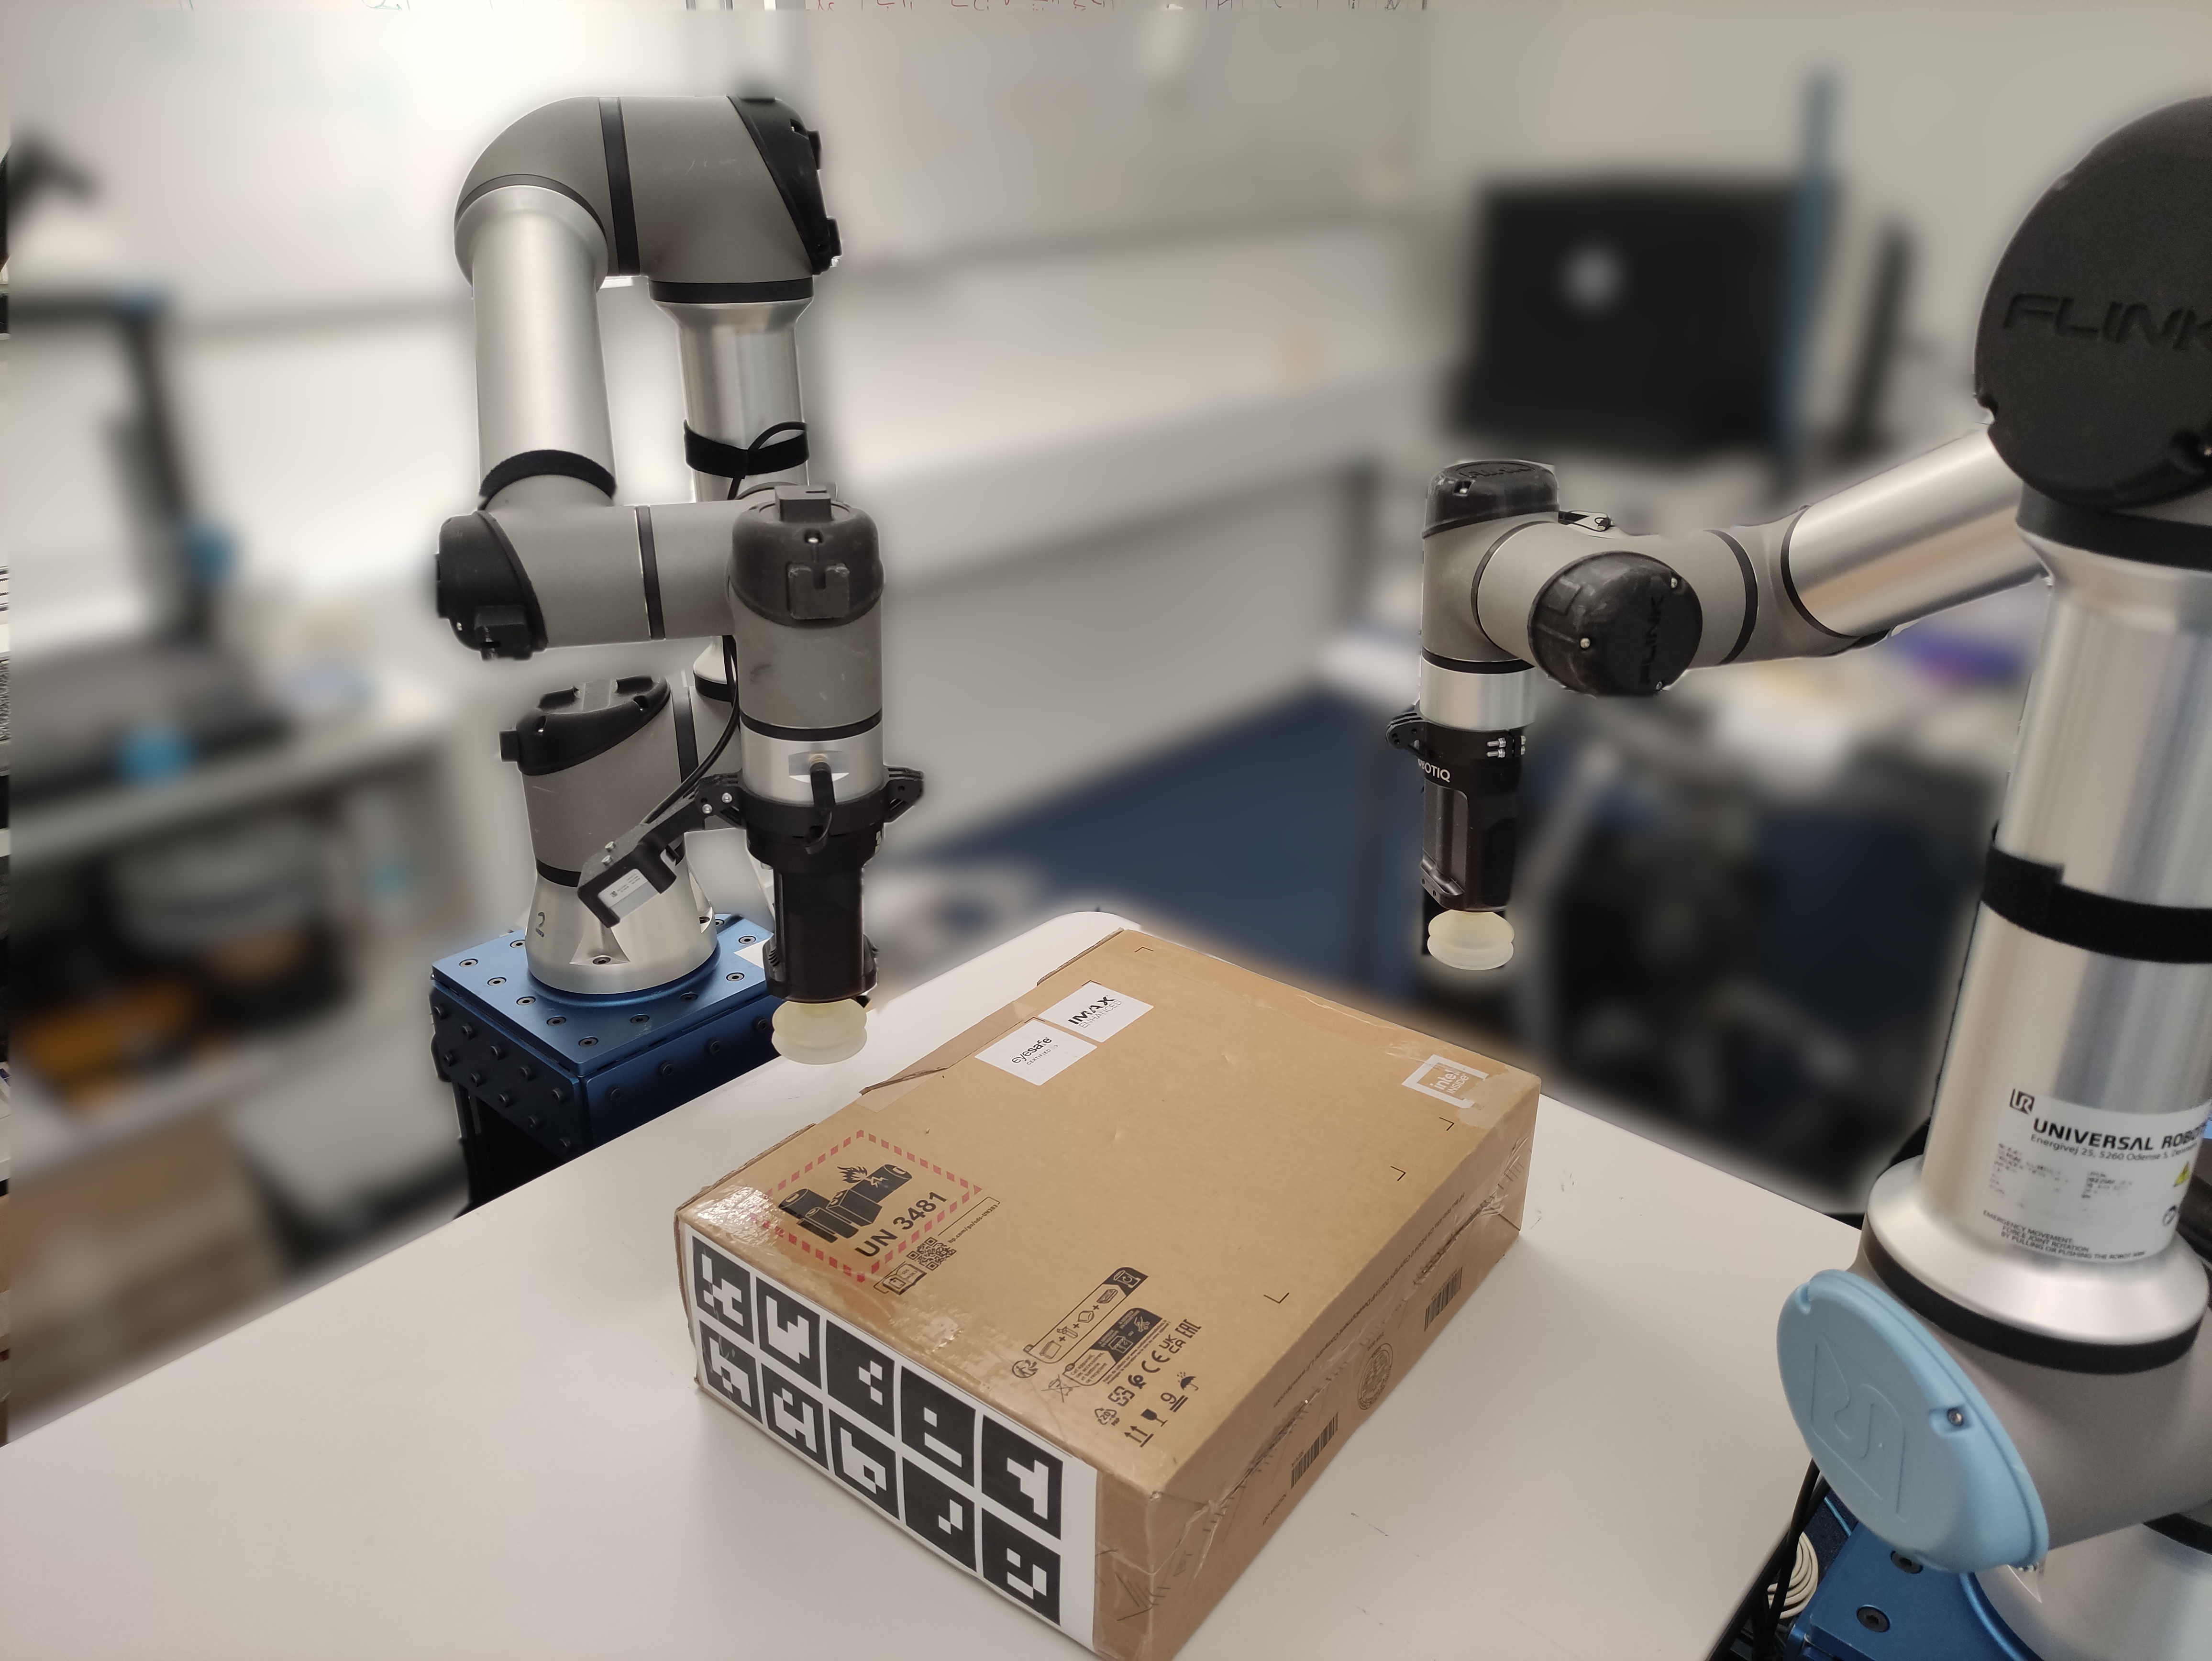
\includegraphics[width=0.65\linewidth]{images/top_blurred.jpg}}
    \subfigure[]{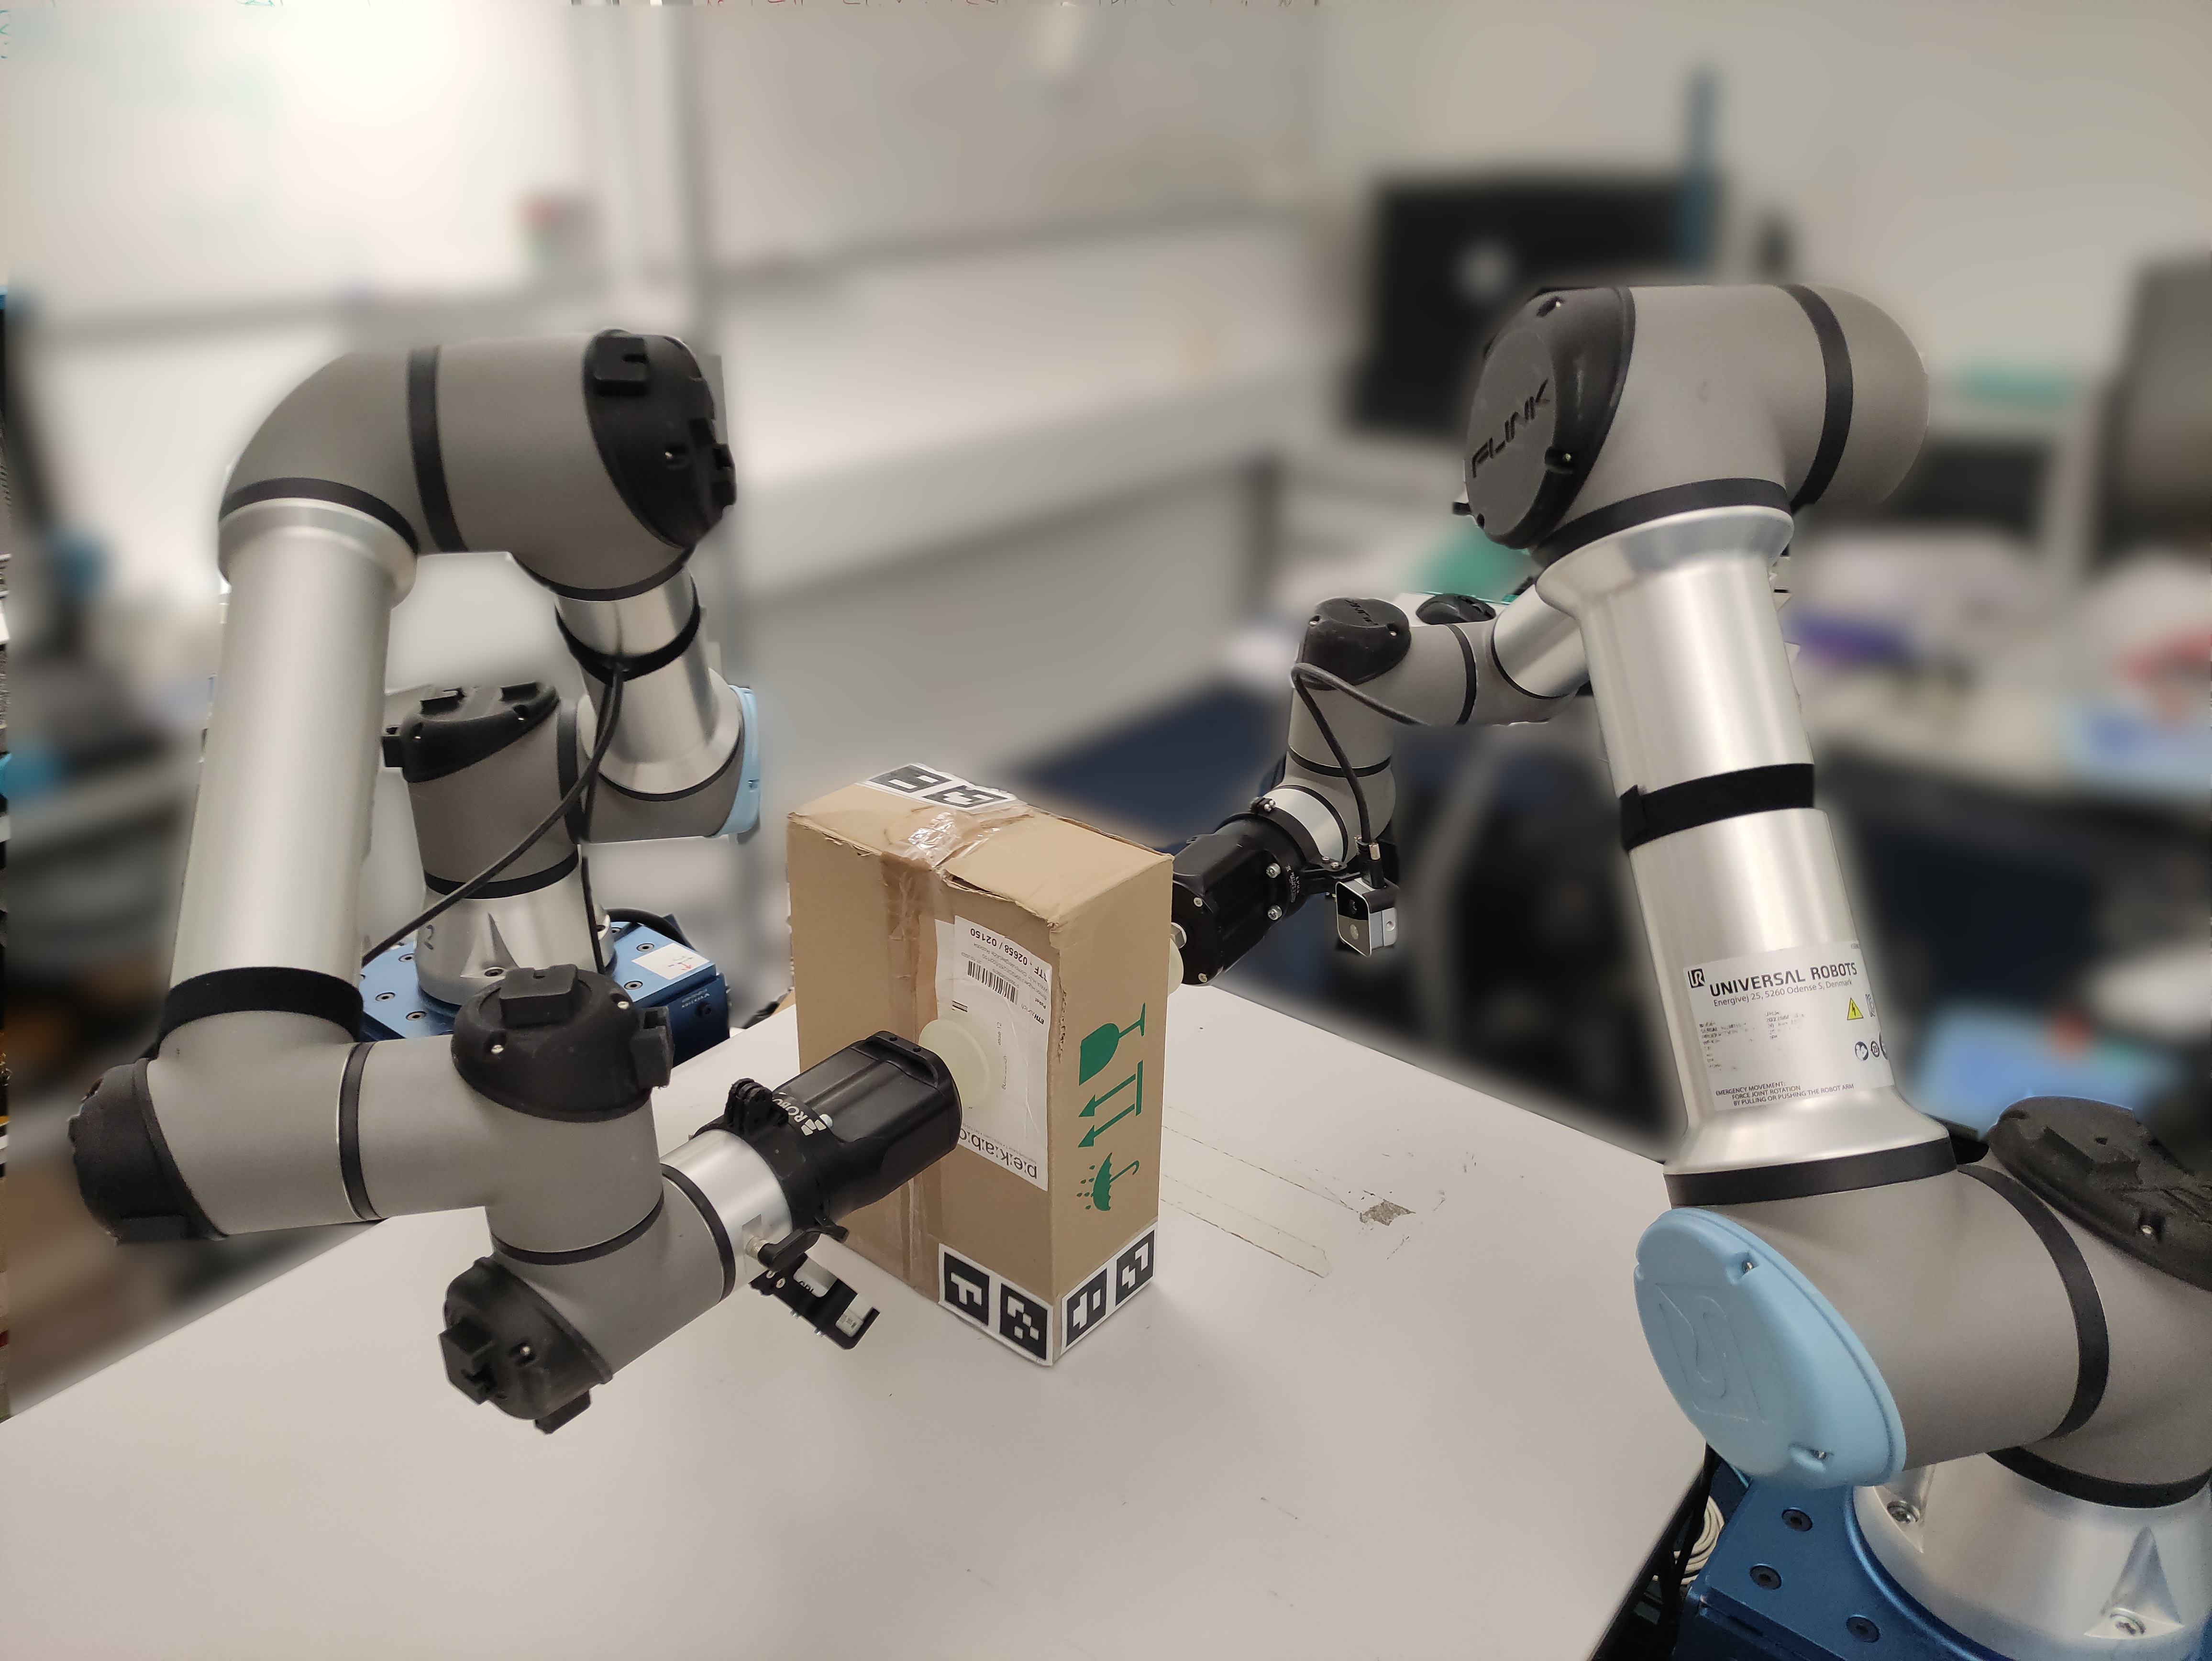
\includegraphics[width=0.65\linewidth]{images/side_blurred.jpg}}
    \caption{In (a), two robots in the \textit{top-grasping} configuration. In (b), the \textit{side-grasping} configuration.}
    \label{grasping-strategy}
\end{figure}

Creating a benchmark for dual-arm manipulation requires selecting possible tasks that robots must perform.
Considering the necessities faced more commonly in logistics centers, we trained policies to:

\begin{enumerate}
    \item lift a box,
    \item rotate a box around one of its axes,
    \item combine a lift and a rotation of a box,
    \item move a box to different positions inside the workspace.
\end{enumerate}

The differences in the task complexities require different approaches that are covered in the following paragraphs (\cref{visual-info}, \cref{hil}, \cref{her}, \cref{rrl}). A more detailed definition of every policy can be found in \cref{lift}, \cref{rot}, \cref{lift+rot}, and \cref{motion}.

\begin{figure}[t]
    \centering
    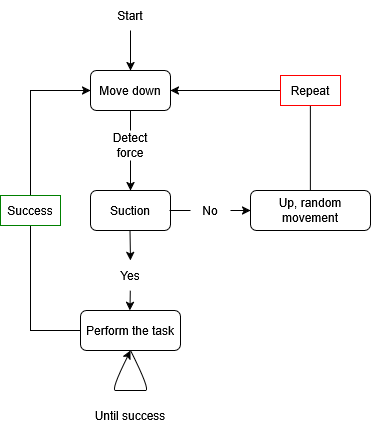
\includegraphics[width=0.99\linewidth]{images/BT_gen.drawio.png}
    \caption{A graph representing a general scheme of a Behavior Tree.}
    \label{BT-strategy}
\end{figure}

The first problem we faced was ensuring the two robots could grasp the object securely without letting it fall.
Initially, two grasping strategies were taken into account (see  \cref{grasping-strategy}).
A so-called \textit{top-grasping} strategy, with the end effectors facing the table surface, and a \textit{side-grasping} strategy, where the end effectors are pointing at each other. 
As one might expect, the choice of the grasping strategy depends on the boxes' dimensions, particularly on which plane lies the longest dimension.

The first idea is to compare the performance of a simple controller against policies trained with Reinforcement Learning. This first controller allowed us to identify possible failure cases that can be fixed by exploiting learning-based approaches. 

\begin{figure*}[t]
    \centering
    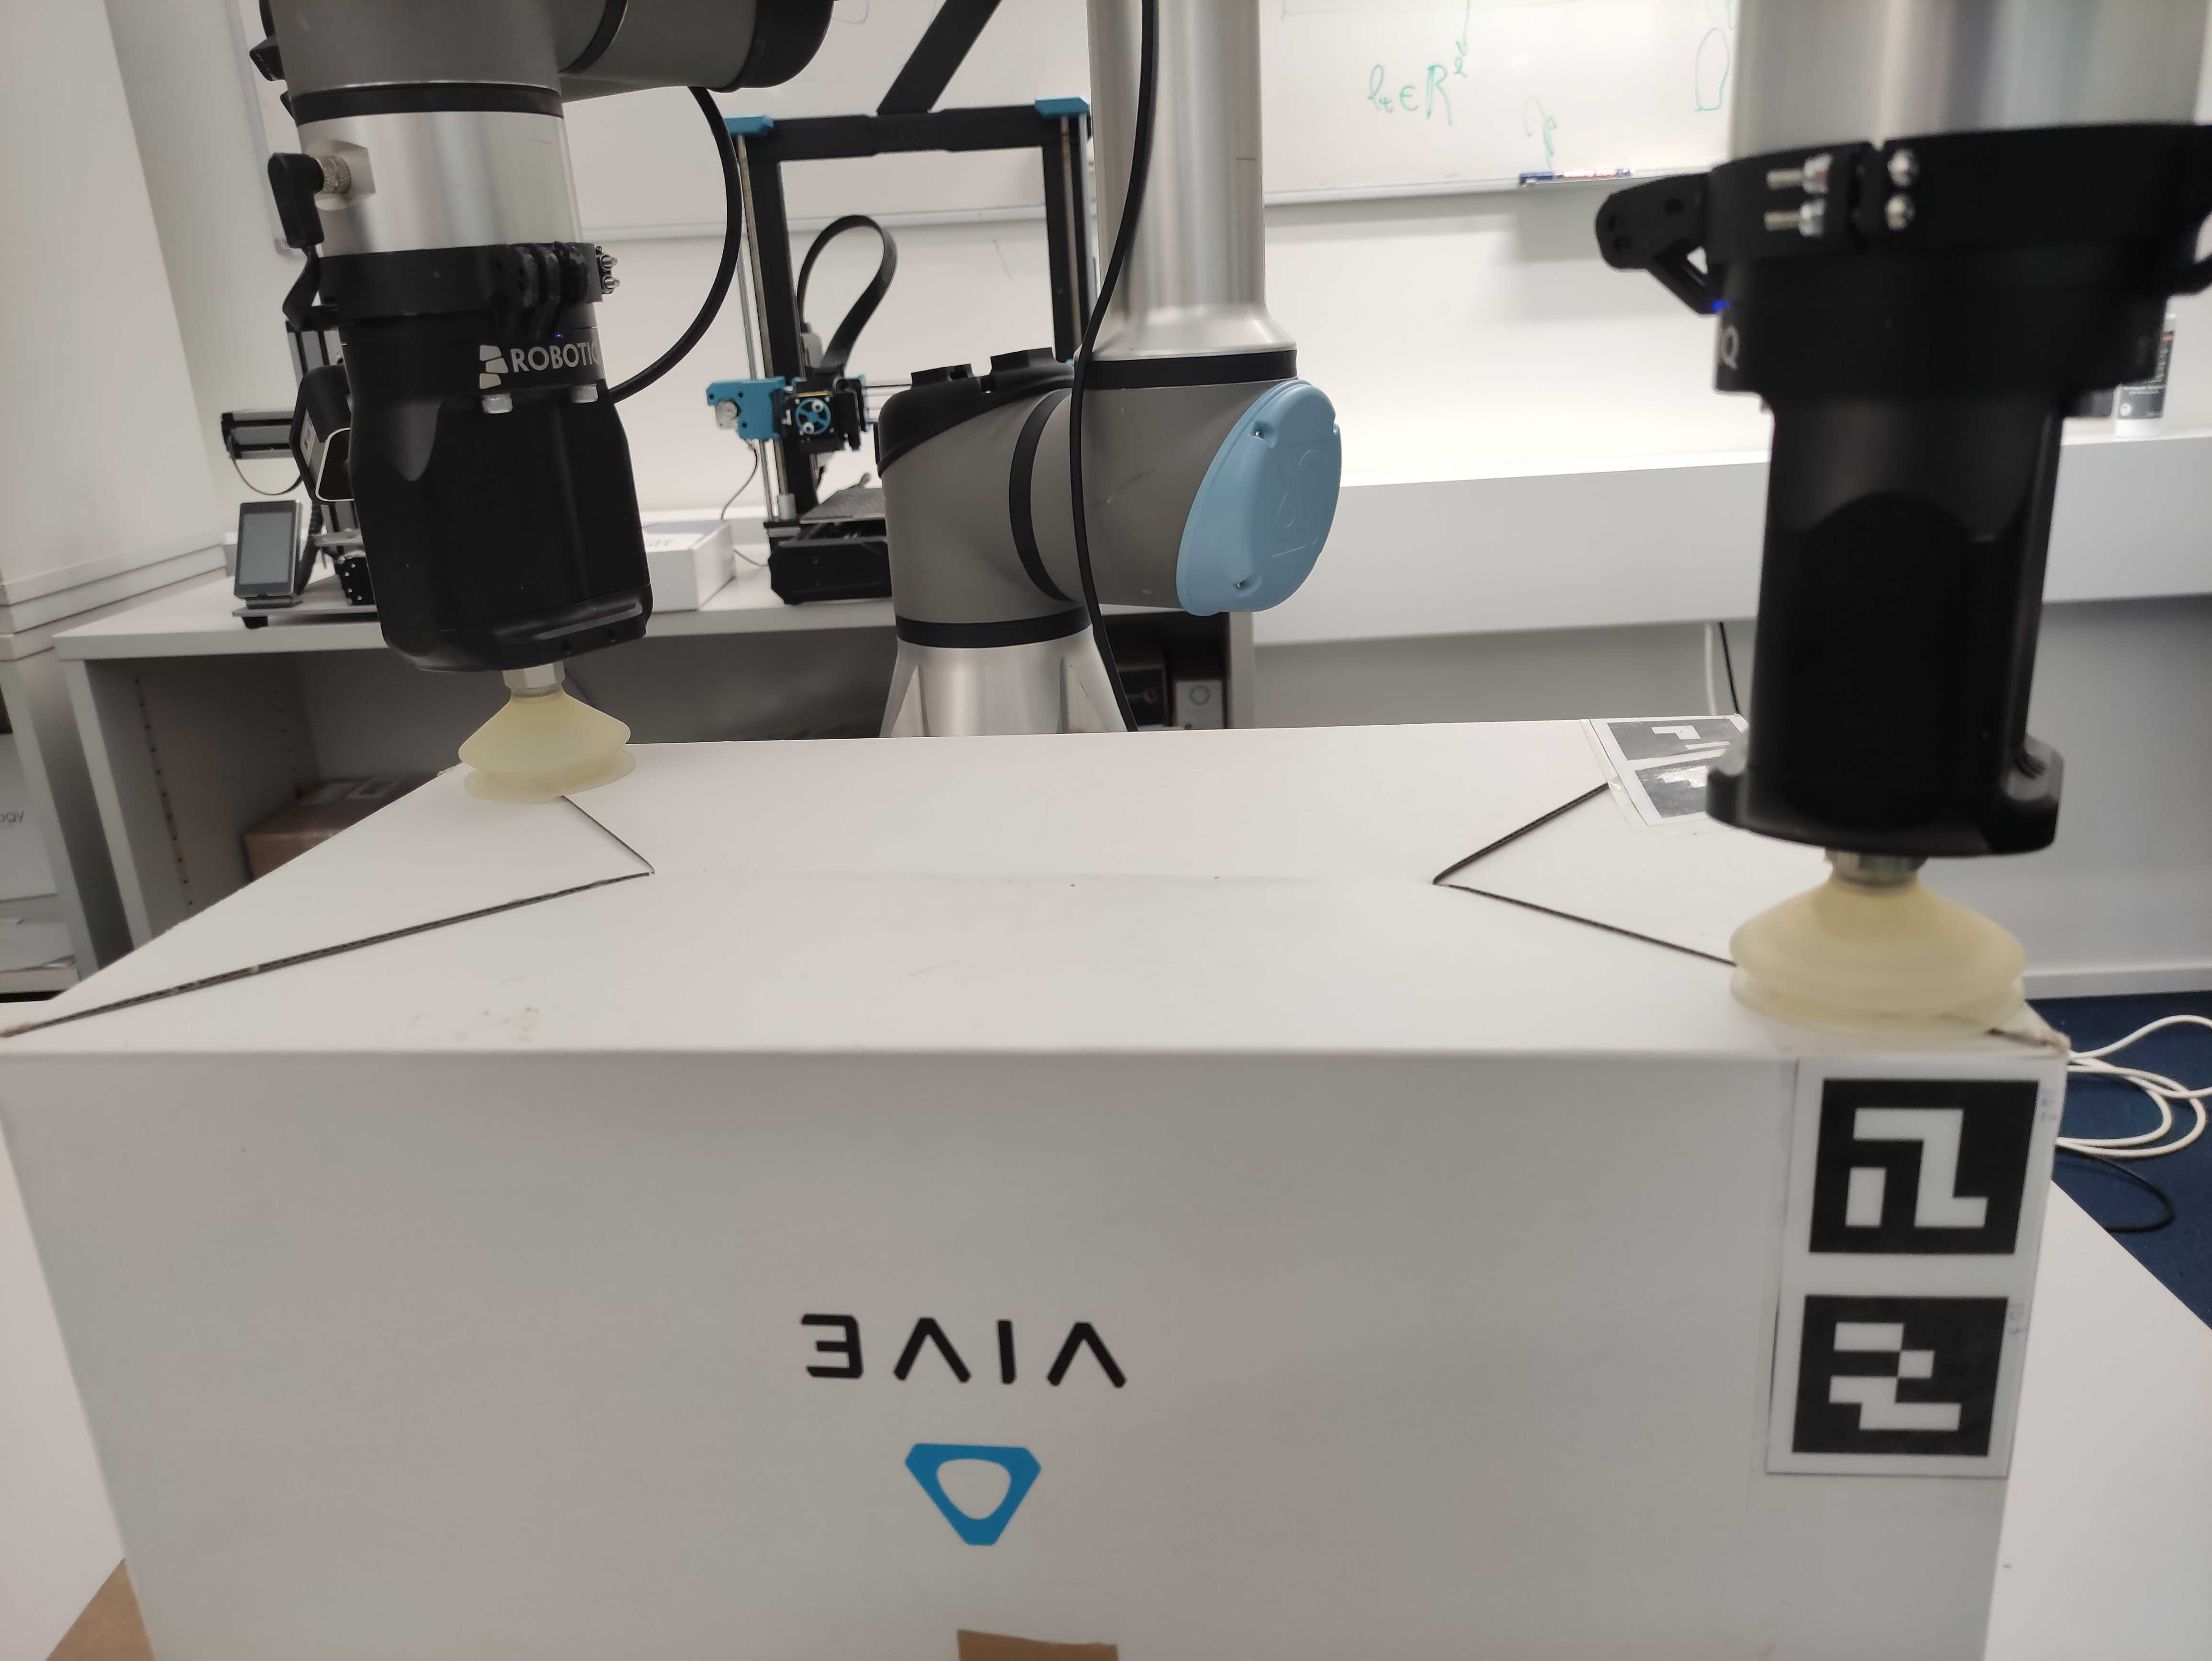
\includegraphics[width=0.24\textwidth]{images/IMG_20250411_100113.jpg}
    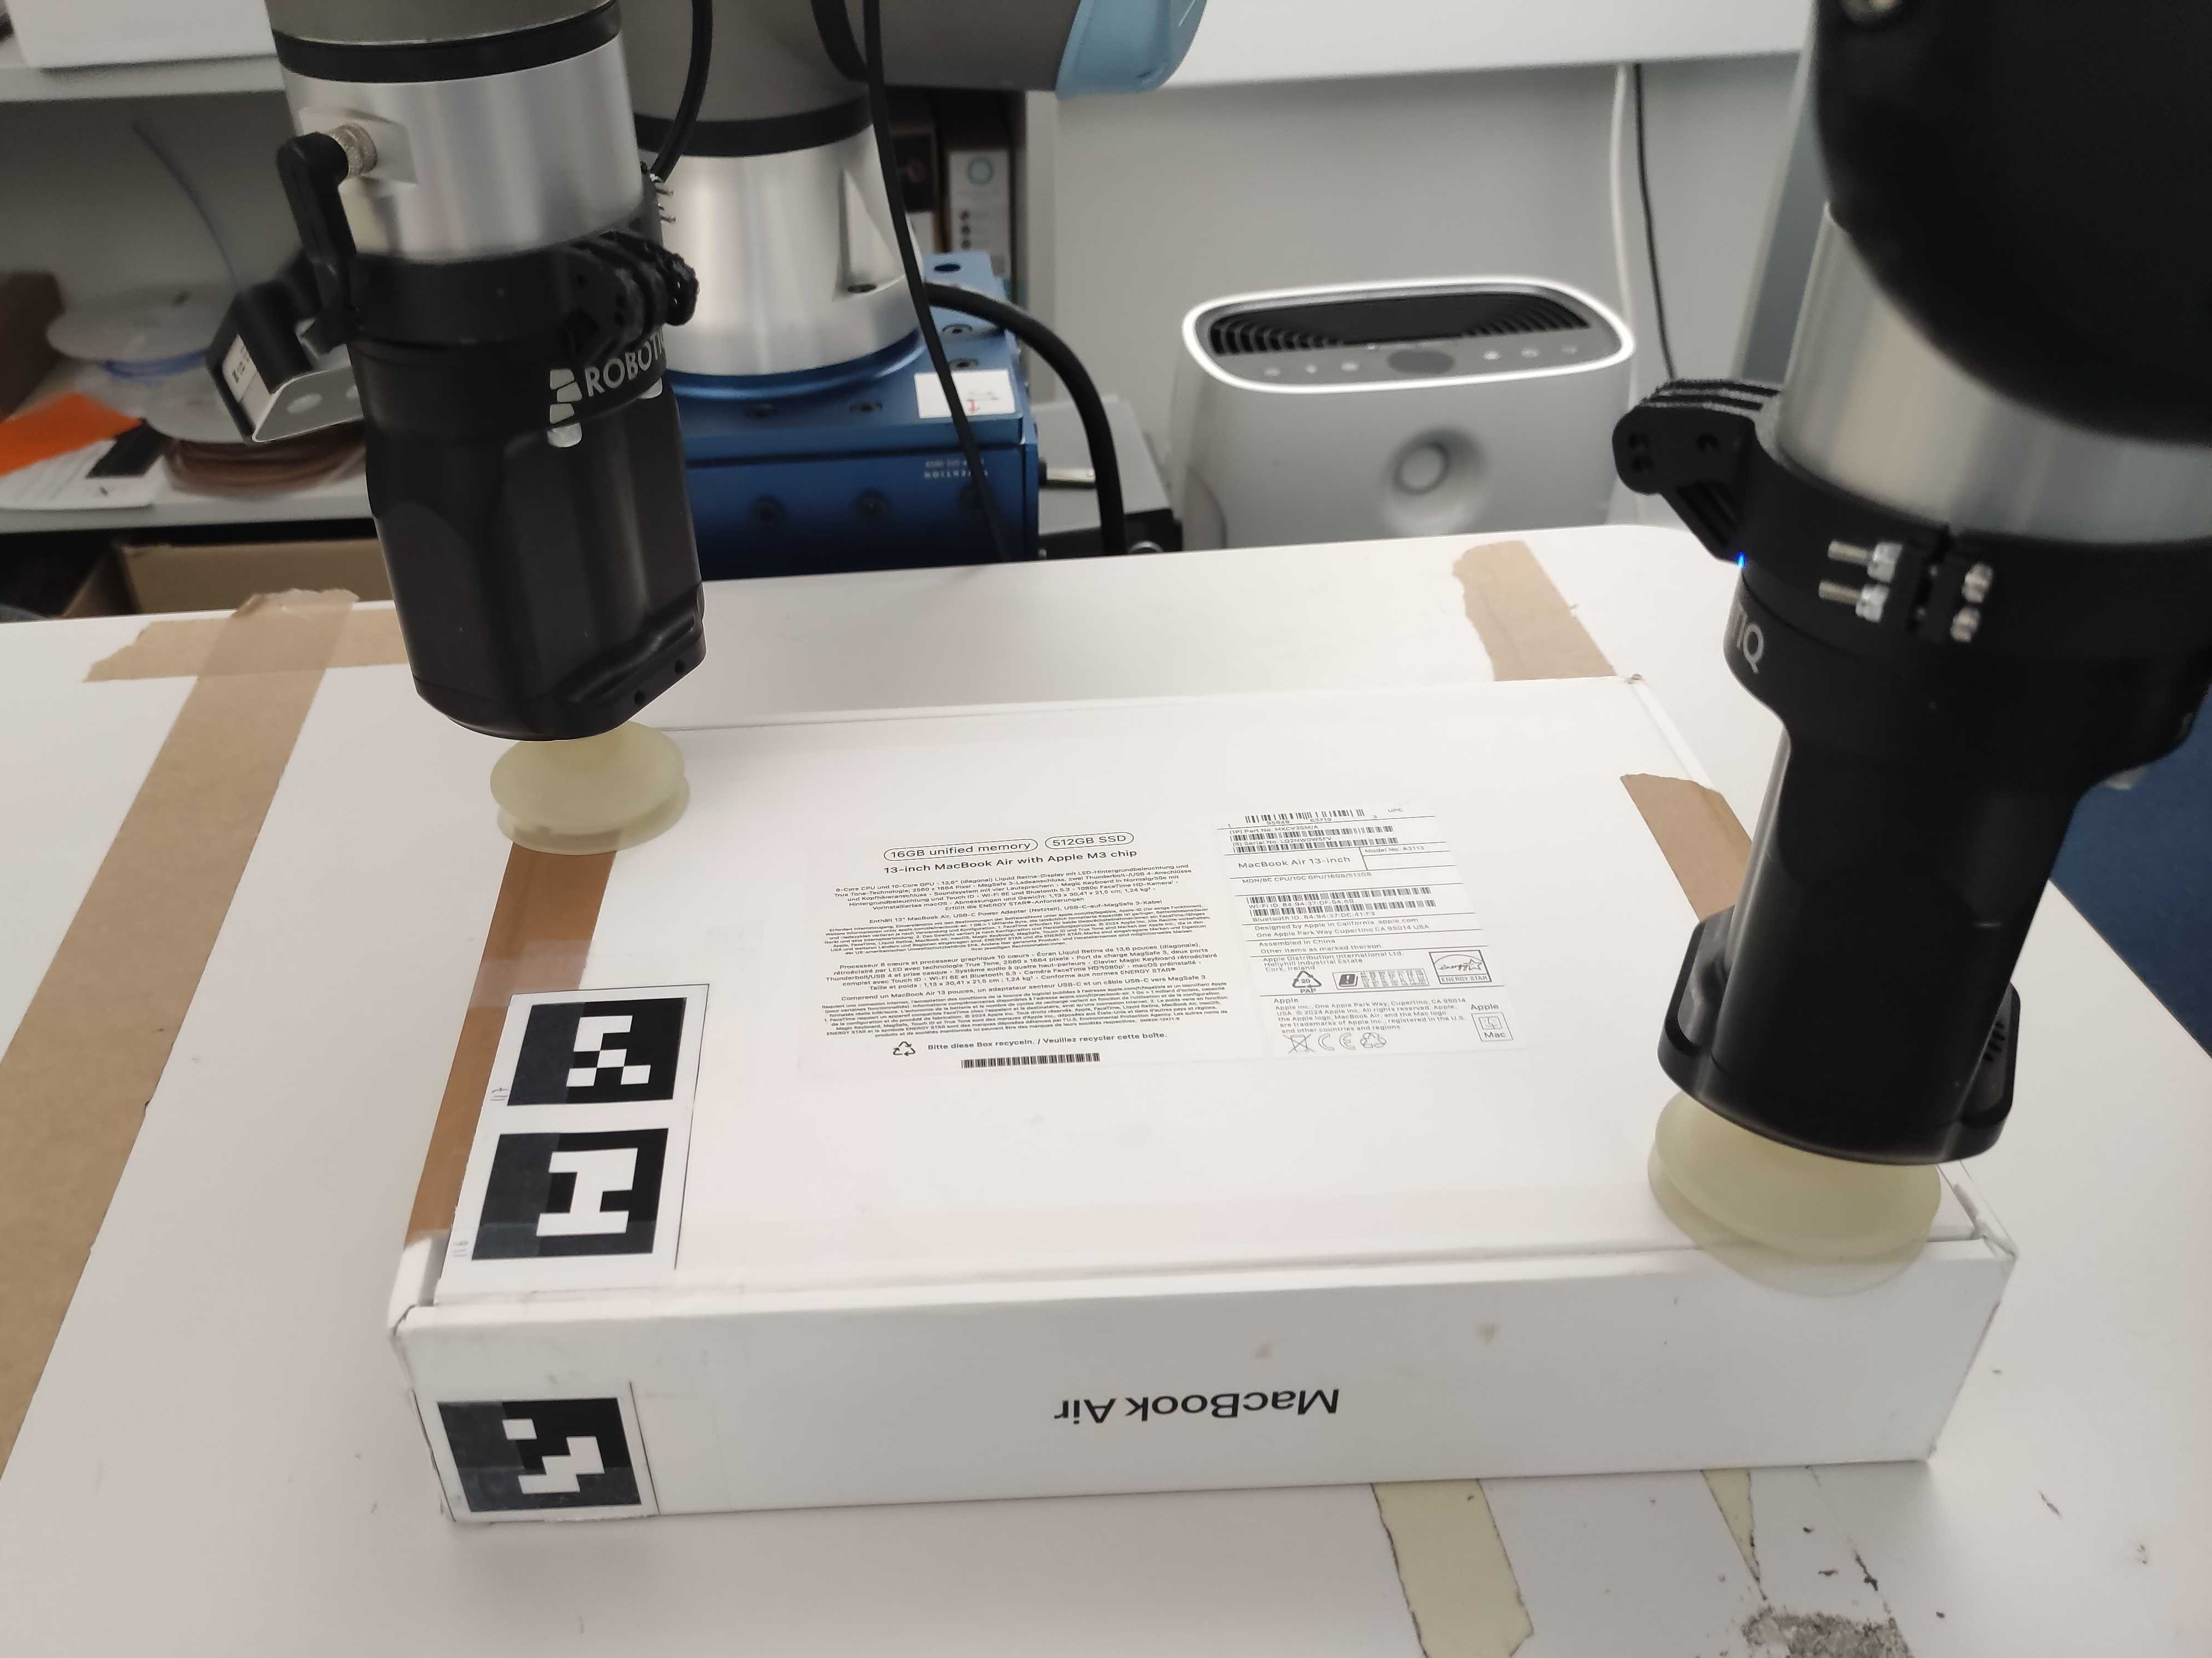
\includegraphics[width=0.24\textwidth]{images/IMG_20250411_100317.jpg}
    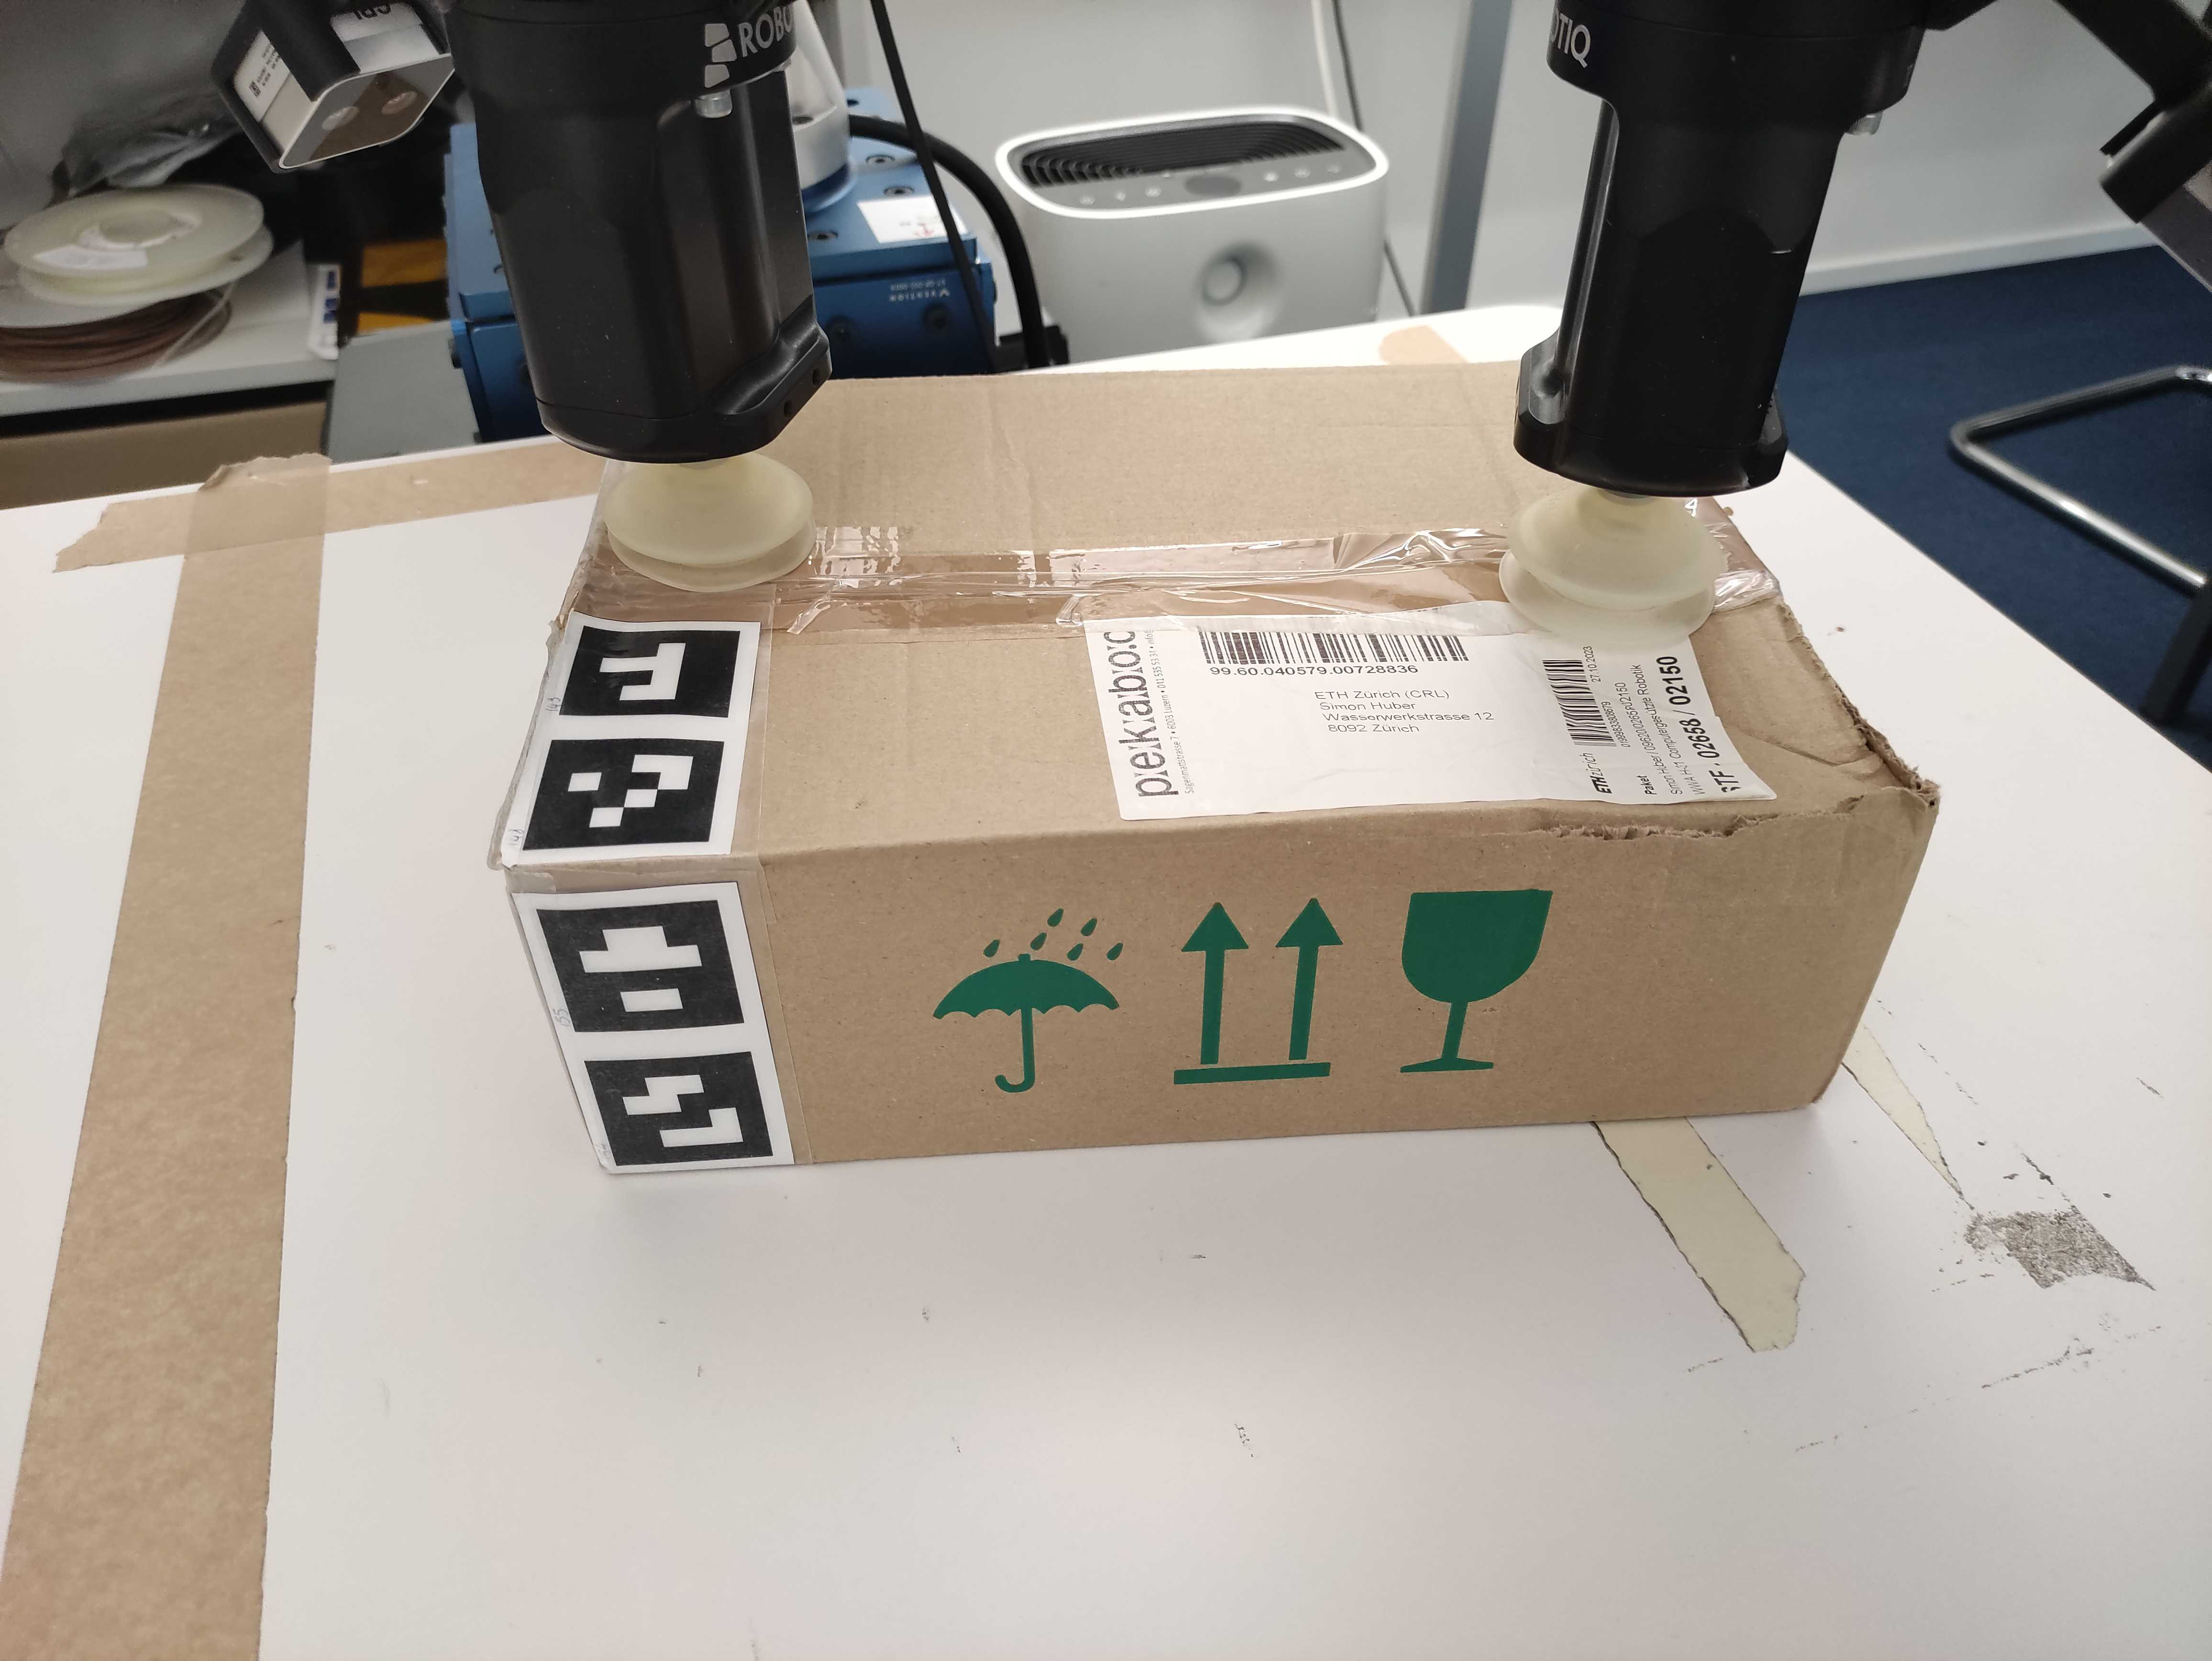
\includegraphics[width=0.24\textwidth]{images/IMG_20250411_100932.jpg}
    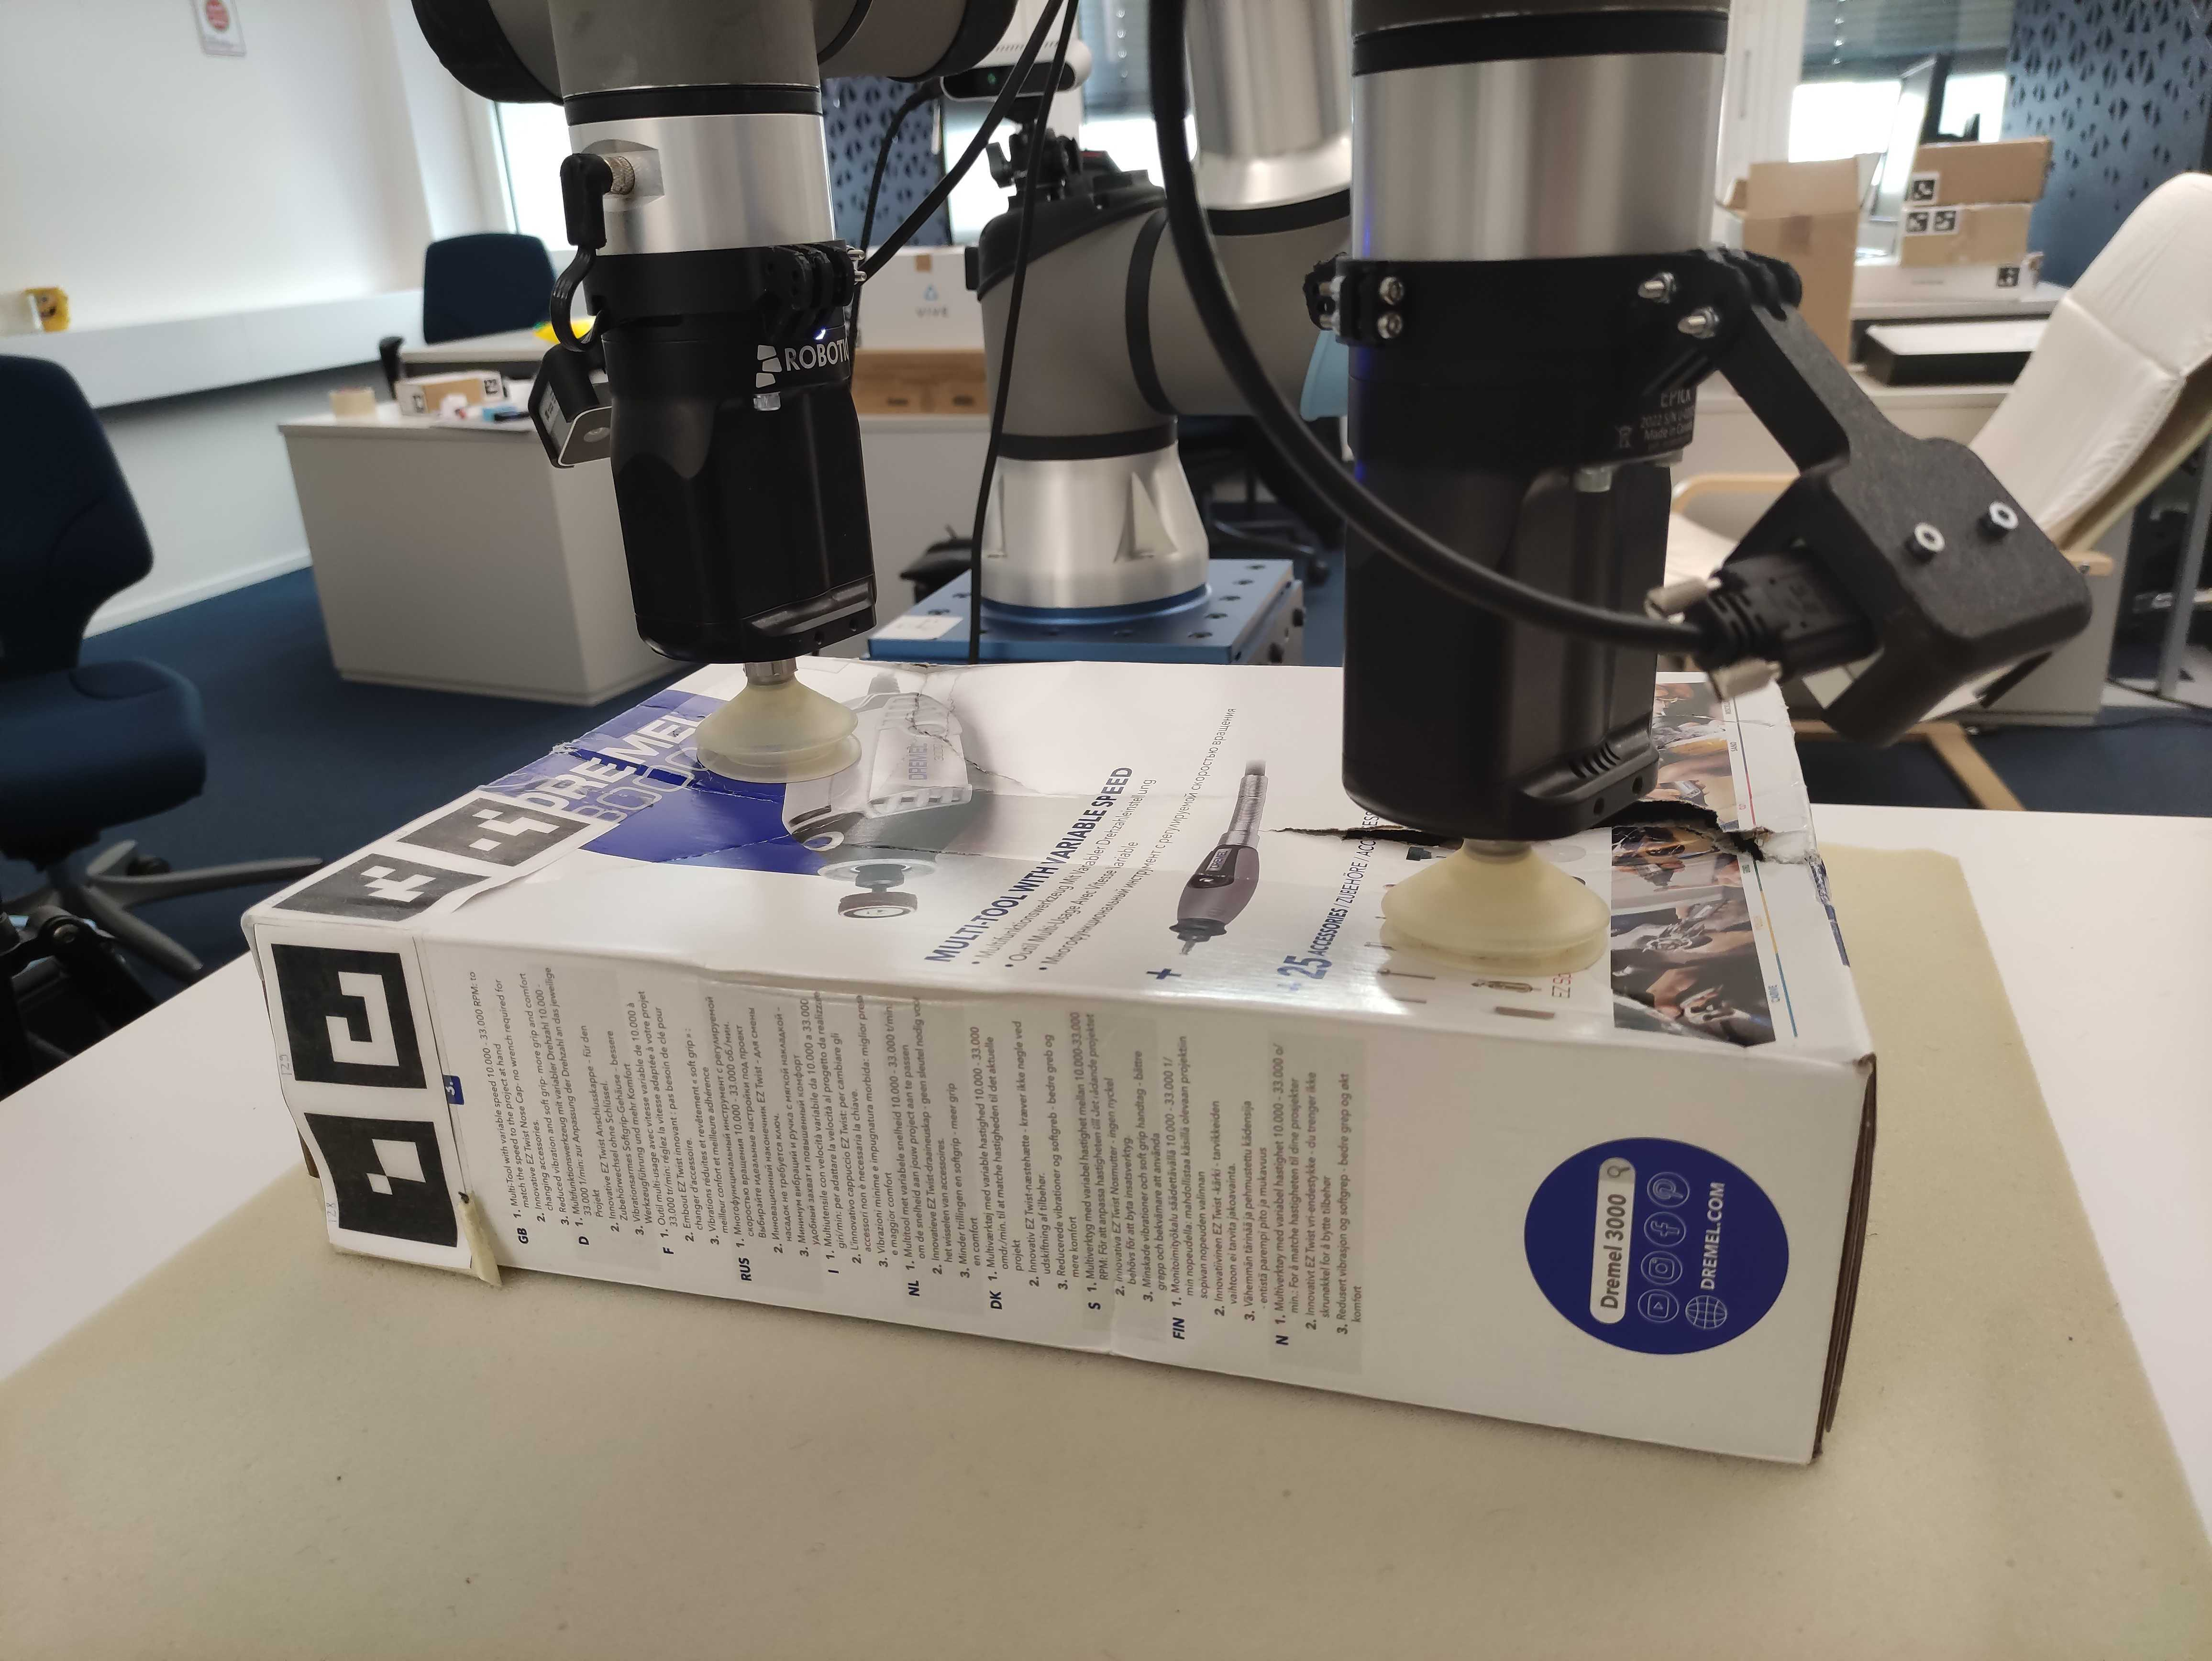
\includegraphics[width=0.24\textwidth]{images/IMG_20250414_103423.jpg}
    \caption{Possible failures in the grasping of a box. Holes, tape, and broken parts make grasping challenging.}
    \label{failures}
\end{figure*}

For example, we created a controller based on a behavior tree (BT) to perform the desired tasks and establish the first baselines (see \cref{BT-strategy}). 
%These can be easily deployed on a real setup without using pose estimation or any learning-based approach.
It is straightforward to realize that policy performance may vary. 
We observed that suction cups struggle when grasping boxes that are covered with tape or that present holes on their surface (see \cref{failures}). Small changes in the box's initial position and orientation have a huge influence, too. 

% Furthermore, it was noted that UR5e robots fall into a singularity configuration, called wrist alignment singularity, typical of their kinematic structure. When 4 joint axes are parallel, which happens frequently when \textit{side-grasping} is used. This happens when the shoulder, elbow and wrist 1 joints rotate in the same plane. 
% However, when we also align the movement of wrist joint 2 with this same plane by moving it to an angle of 0 or 180 degrees, we limit the range of movements of the robot, regardless of the area of the workspace. 
% Due to the issues with the singularity configuration, we decided to focus solely on grasping approaches based on the \textit{top-grasping} strategy.

For the sake of simplicity and considering the relative positions of the robots, in this work, we considered only the \textit{top-grasping} strategy.

% TODO: reformulate this part as singularities can be avoided by just switching to a velocity controller. It can be removed too. To justify the choice of the grasping strategy, just say "for this work, we focused on top-grasping only

\subsection{Integrating visual information}\label{visual-info}
Visual information is fed into the policy's neural network to provide local information about the box. It was shown that these enhance the adaptability of the policy to different boxes \cite{kostrikov2021imageaugmentationneedregularizing}. Several visual backbones can be adopted in SERL, including, for example, grey or RGB images with ResNet. Voxel-SERL integrates a voxel-grids-based method, which showed an increase in performance over the previous methods \cite{sutter2025comparisonvisualrepresentationsrealworld}.
The visual inputs are taken from a camera mounted on each wrist of the robot and then processed by a neural network.
Training lasts longer when visual information is added to the observation space of the policy. While running the experiments, we noticed that RLPD tends to explore more than a simple SAC algorithm, taking more time to converge. 
We realized that this exploration originated issues with collisions between the robots and singularity configurations, which were not encountered during the training without wrist camera information. 
% TODO:  underline that this is your experience, not a result or a citation to a paper

Therefore, the system must frequently check if it is in a collision or singularity configuration. The former is evaluated by computing the relative 2-norm distance between the tip of the gripper, the end-effectors, and the 5th and the 4th joints of the two robots, the latter is avoided by shrinking the workspace of the robots. 

In order to avoid actions that move the robots into a collision or a singularity, during training we penalized the agent if the robots were getting too close, leading to the end of the episode too. In addition, a custom reset procedure is needed to avoid collisions once the end of the episode is reached.
When training policies using RLPD, we introduced an additional cost on the relative end-effector distance. 
% A larger penalty is needed when the end-effectors are closer.

% After several unsuccessful experiments, we found out that adding human interventions was the key element to achieving successful policies within a reasonable training time. A clear and detailed description of what human interventions are is presented in \cref{hil}.

\subsection{Introducing human interventions}\label{hil}

\begin{figure}[t]
    \centering
    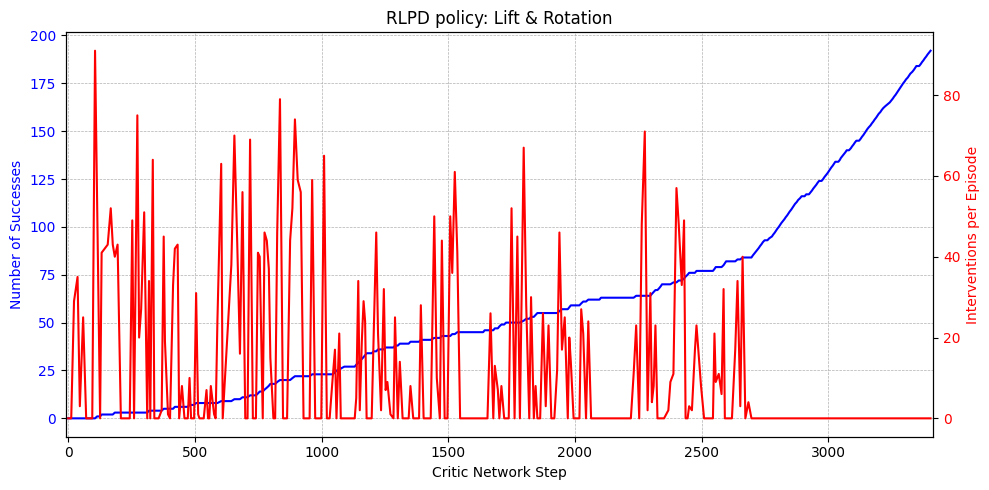
\includegraphics[width=1\linewidth]{images/hil.png}
    \caption{Number of human interventions per episode compared to the number of successes performed during the training of the RLPD policy that performs a lift combined with a rotation of the box.}
    \label{hil-plot}
\end{figure}

The complexity required to train reinforcement learning policies is closely linked to the cardinality of the state and action spaces, as well as the task horizon, assuming an appropriate exploration policy (\cite{jin2018qlearningprovablyefficient}, \cite{jin2019provablyefficientreinforcementlearning}, \cite{azar2012samplecomplexityreinforcementlearning}, \cite{kearns2002near}). Increases in the size of the state/action spaces, task horizon, or their combination lead to a proportional rise in the number of samples required to learn an optimal policy. This can eventually make online reinforcement learning impractical. 
Those challenges can be overcome by allowing a human operator to guide the learning process by intervening at random steps during training. This is what \cite{luo2024precisedexterousroboticmanipulation} refers to as \textbf{human-in-the-loop feedback}.

More in detail, a human operator supervises the robot during training and provides corrective actions to explore more efficiently. Interventions can be easily performed by acting on the SpaceMouse. When a human intervenes, the action read from the SpaceMouse is applied to the robot instead of the policy's action.

Unlike the implementation available in \cite{luo2024precisedexterousroboticmanipulation}, one single replay buffer is used in all tasks except the motion. In those tasks, the policy's transitions are added to the buffer together with the interventions.

Using human interventions can massively speed up the training, but it comes with some negative drawbacks too. As can be quickly realized empirically, providing long and sparse interventions that lead to task success will cause the overestimation of the value function. This happens in particular when interventions are frequent in the early stages of the training process. These result in unstable training dynamics.

In our experience, the policy improves faster when the human operator issues specific corrections while letting the robot explore on its own otherwise. 
In  \cref{hil-plot}, one can visualize the number of interventions per episode performed together with the number of successes during the training of a policy to lift and rotate a box. Once the policy becomes good enough, the number of successes grows even without human interventions.

Considering the lifting task as an example, intervening just to correct wrong behaviors while learning to grasp or lift keeps the training stable and guides the exploration towards a correct and successful policy. 
%Act first to perform a correct grasp and correct the lift only in the following episodes, once a correct grasp is correctly achieved.

\subsection{Hindsight Experience Replay (HER)} \label{her}

\begin{algorithm}[t]
    \scriptsize
    \caption{Integrating HER in the training loop}
    Initialize demo buffer $\mathcal{D}$\\
    Replay buffer $\mathcal{R} \gets \emptyset$\\
    Sample a goal $g$\\
    Transitions $trans \gets \{\}$\\
    HER Transitions $her\_trans \gets \{\}$\\
    \For{episode=1,M}{
        \For{t=1,N}{
        $trans \gets \{s_t, a, r(s_t,a, g),s_{t+1}\}$\;
            \If{episode finishes}{
                $g_{her} \gets p^{box}$\Comment*{Define new goal}
                \eIf{episode is successful}{
                    $\mathcal{R} \gets \{trans\}$\;
                }{
                    $her\_trans \gets  \{s_t, a, r(s_t,a, g_{her}),s_{t+1}\}$\Comment*[r]{Recompute transitions}
                    \eIf{new episode is successful}{
                        $\mathcal{R} \gets \{trans\}$\;
                        $\mathcal{R} \gets \{her\_trans\}$\;
                    }{
                        $\mathcal{R} \gets \{trans\}$\;
                    }
                }
            }
        
        }
        $trans \gets \{\}$\;
        $her\_trans \gets \{\}$\;
    }
    \label{her_algo}
\end{algorithm}

Considering the motion planning task, we needed a smart strategy to record demonstrations to bootstrap the training of the reinforcement learning policy. There are two main problems: knowing the goal position before actually reaching it, and moving the box toward this location. To simplify this step, we implemented \textbf{Hindsight Experience Replay} \cite{andrychowicz2018hindsightexperiencereplay}. In this paper, HER is implemented to train control policies in a simulation that accomplish three manipulation tasks: pushing, sliding, and pick-and-place. Another work used HER together with demonstrations in a single-arm setup to solve a block stacking task \cite{nair2018overcomingexplorationreinforcementlearning}. Similarly to our scenario, the replay buffer was initialized with 100 human-expert demonstrations, but the final policy was only trained and evaluated in simulation. HER was integrated only during training to profit from the experience gained from unsuccessful episodes.

During the recording, one can sample a goal position inside the dual-robot workspace. In the beginning, this goal position is used as a \textit{fake} goal. This means that we do not know exactly where the goal is, but we still compute rewards and observations based on it. 
So, the boxes are just moved randomly inside the workspace. At the end of the recording of every demonstration, the final box position is considered as the \textit{real} goal position, and all the rewards and observations are recomputed according to this goal.

At the end of all the unsuccessful episodes, we collect two sets of transitions. One in which the goal is not actually reached and one in which the goal is achieved. The latter are saved in the replay buffer and used to bootstrap the training.
The same post-processing strategy is used at training time, as explained in Algorithm \ref{her_algo}. 
When training the policies, two sets of transitions are saved in the replay buffer only when the episode ends unsuccessfully, but the box was grasped at least in the last step.
This choice aimed to reduce the number of unsuccessful transitions in the replay buffer, in particular during the early steps of the training. 
Hindsight Experience Replay is not needed when the box is not grasped or the episode ends successfully.

\subsection{Residual Reinforcement Learning (RRL)}\label{rrl}
\textbf{Residual Reinforcement Learning} \cite{johannink2018residualreinforcementlearningrobot} represents a variation of traditional learning-based techniques. To take advantage of the efficiency of conventional controllers but also the flexibility of RL, the control action is defined as:
\begin{equation}\label{control_rrl}
    u=\pi_H(s) +\pi_\theta(s)
\end{equation}
where $\pi_H(s)$ is a human-designed feedback control law and $\pi_\theta(s)$ is a learned policy parametrized by $\theta$ and optimized by an RL algorithm to maximize the expected returns on the task.
This approach simplifies the training of the secondary policy and enables its use as an optimizer for the primary one. Other works in manipulation substitute the human-designed feedback control law with a BC policy \cite{ankile2024imitationrefinementresidual}.

In this work, we integrated RRL only in the motion task to guide the robotic arms toward the desired goal position. The control action applied to the robots is computed as follows:
\begin{equation}\label{action_Residual}
    u_t=(a_{FF_{t}}+a_{t})\cdot k
\end{equation} % use \bar a instead of u (RL convention)
where $a_t$ is the action at time t, $a_{FF_{t}}$ is the feed-forward action, which in our case is the normalized vector representing the direction that connects the goal position to the actual box position, and $k$ is the scaling factor. 
When recording the demonstrations, $a_t$ is the SpaceMouse command, while during training, it is the output of the actor network.

\section{EXPERIMENTS}

\begin{figure*}[t]
    \centering
    \subfigure[]{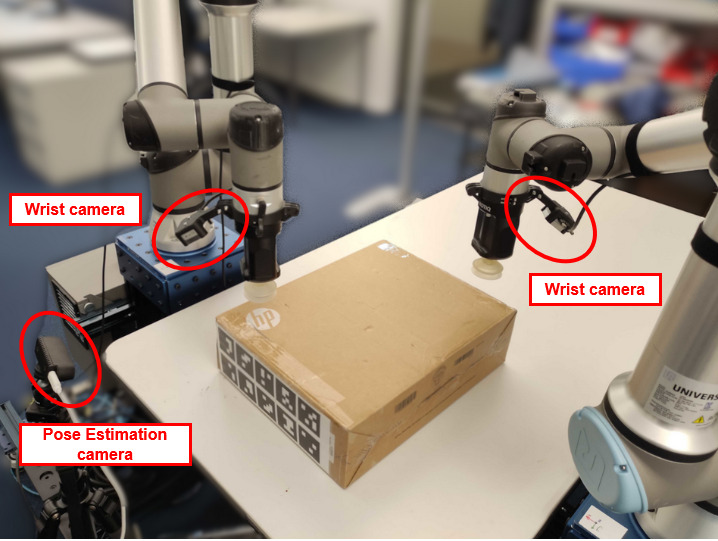
\includegraphics[width=0.461\linewidth]{images/setup_blurred_commented.jpg}}
    \subfigure[]{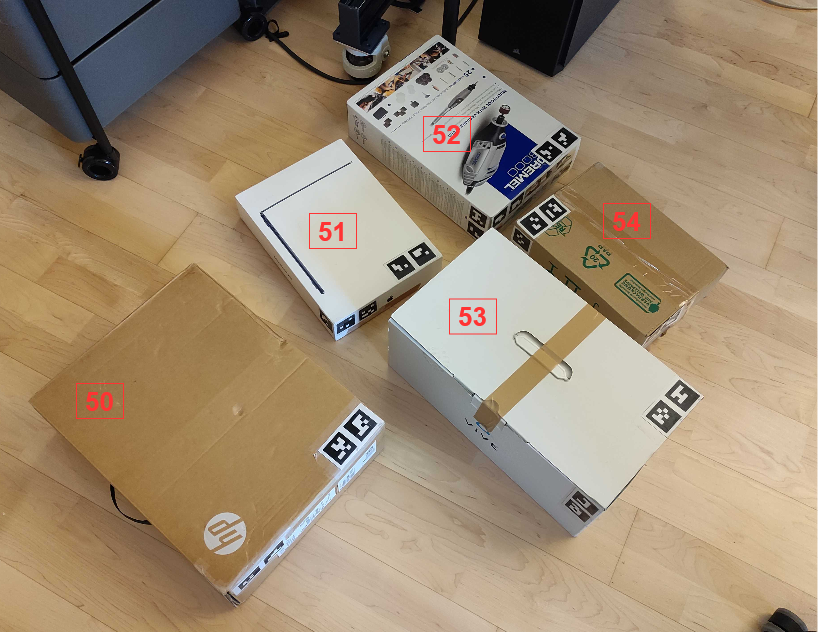
\includegraphics[width=0.45\linewidth]{images/boxes_id_bugger.drawio(1).png}}
    \caption{In (a), the setup used for the experiments. In (b), the boxes used during policy evaluation.}
    \label{Setup_and_boxes}
\end{figure*}


\begin{table}[t]
    \centering
    \caption{The dimension of the boxes used during training and evaluation.}
    \renewcommand{\arraystretch}{1.5}
    \begin{tabular}{c|ccc|c}
    \toprule Box ID & X [mm] & Y [mm] & Z [mm] & Group \\
    \midrule 50 & 342 & 452 & 130 & Seen \\
     51 & 245 & 335 & 72 & Unseen \\
     52 & 268 & 391 & 102 & Unseen \\
     53 & 249 & 431 & 189 & Unseen \\
     54 & 221 & 310 & 105 & Unseen \\
    \bottomrule 
    \end{tabular}
    \label{box-dim}
\end{table}

For the experiments, we used two 6-DoF UR5e Robot Arms, each one with the Robotiq EPick vacuum gripper. The demonstrations were recorded using two separate SpaceMouses. On the wrist of the end-effectors, we placed an Intel RealSense D405 camera for each arm to augment the vision capabilities. Additionally, an Orbbec Gemini RGBD camera is used for the pose estimation of the boxes (see  \cref{Setup_and_boxes}). 
This camera is only used in a separate thread to detect the position of the box via ArUco tags \cite{GARRIDOJURADO20142280}.

A simple behavior tree is used as a baseline for every task. Policy training was done using just one box (ID=50). Each RL-based policy was initialized with 20 successfully teleoperated demonstrations, except one of the motion planning policies, which was initialized with 60 demonstrations, as we will discuss in \cref{motion}. 

The policies' performance must be evaluated in different scenarios while handling boxes of different dimensions, weights and shapes. These boxes are visualizable in  \cref{Setup_and_boxes}. The sizes of the boxes are reported in \cref{box-dim}. 
It is worth mentioning that some physical properties of the boxes can be unknown or hard to estimate. No information about the weight of the box, the dimensions, the friction coefficient, or the location of the center of mass is considered as an input. For example, Box 50 contains several smaller boxes inside itself, so the location of the center of mass is variable over time and across different episodes.

A pre-trained VoxNet is adopted as a visual backbone to augment the observation spaces when running the RLPD algorithm.

A brief description of each task can be found in the \cref{lift}, \cref{rot}, \cref{lift+rot}, and \cref{motion}. All the observations and rewards are reported in the appendix (\cref{appendix}). We note that all the angles are represented using Modified Rodrigues Parameters. %TODO: add citation
The evaluation metrics are (1) \textbf{the success rate}, which is 1 for a successful episode and 0 for a failure with no partial credits; (2) \textbf{a set of sub-successes} that characterize every task; (3) the \textbf{time} it takes for a trajectory to reach the goal state or time out.

\subsection{Lift policy}\label{lift}

The first task is to lift a box by 5 cm. In more detail, the success condition is achieved when both robots are grasping the box, and the actual robot's TCP positions are 5 cm higher than the robot's initial TCP positions.

This task is the only one that does not integrate the box position into the observations. The observation space, the reward weights, and the success condition are reported in \cref{lift_obs} and \cref{lift_rew_sac}.

\subsection{Reorientation policy}\label{rot}

The second task is to rotate a box around its z-axis. The initial orientation of the box can be estimated using the vision system. Then, a \SI{40}{\degree} rotation of the box is achieved using the \textit{top-grasping} configuration. 
The observation space, the reward weights, and the success condition must be changed accordingly, as shown in \cref{rot_obs}, \cref{rot_sac_rew} and \cref{rot_drq_rew}. 
More in detail, a positive reward is given for an anti-clockwise rotation of the box. When tuning the rewards, we found that computing the relative rotation using angles expressed in angle-axis representation improved the results. The success condition is achieved when both robots are grasping the box, and the box has rotated \SI{40}{\degree} around the z-axis from its initial position.

\subsection{Combining lift and reorientation}\label{lift+rot}
The third task is a combination of the two previous tasks, i.e. lifting the box for about 5 cm and rotating it around one axis at a random angle (sampled between \SI{15}{\degree} and \SI{25}{\degree} at the beginning of every episode).
The observation space, the reward weights, and the success condition must be changed accordingly, as shown in  \cref{inair_obs}, \cref{inair_sac_rew}, \cref{inair_drq_rew}. 
The success condition is achieved when both robots are grasping the box, and the box has been correctly lifted and rotated from its initial position.

%%%%%%%%%%%
\begin{table*}[t]
    \centering
    \caption{Policy specifications, training times and conditions.}
    \renewcommand{\arraystretch}{1.5}
    \begin{tabular}{c|c|c|c|c|c|c|c}
        \toprule \textit{\textbf{Task}} & \textit{\textbf{ID}} & \textit{\textbf{Policy}} & \textit{\textbf{Visual Backbone}} & \textit{\textbf{Pose Estimation}} & \textit{\textbf{Training Time}} & \textit{\textbf{HIL}} & \textit{\textbf{Demos number}} \\
        \midrule
         & (1) & BT & \xmark & No & \xmark & No & \xmark \\
        Lift & (2) & SAC & \xmark & No & 12 minutes & No & 20 \\
         & (3) & RLPD & VoxNet & No & 50 minutes & Yes & 20 \\
        \midrule & (4) & BT & \xmark & Yes & \xmark & No & \xmark \\
        Reorientation & (5) & SAC & \xmark & Yes & 12 minutes & No & 20 \\
         & (6) & RLPD & VoxNet & Yes & 50 minutes & Yes & 20 \\
        \midrule & (7) & BT & \xmark & Yes & \xmark & No & \xmark \\
        Lift \& Rotation & (8) & SAC & \xmark & Yes & 12 minutes & Yes & 20 \\
         & (9) & RLPD & VoxNet  & Yes & 90 minutes & Yes & 20 \\
       \midrule  & (10) & BT & \xmark & Yes & \xmark & No & \xmark \\
        Motion & (11) & SAC & \xmark & Yes & 40 minutes & Yes & 60 \\
         & (12) & SAC + RRL & \xmark & Yes & 52 minutes & Yes & 20 \\
         \bottomrule
    \end{tabular}
    \label{policy_specs}
\end{table*}

%%%%%%%%%%%%%%%

\subsection{Motion Planning}\label{motion} % mention the two buffers!!
A more general implementation does not rely solely on a simple lifting policy but includes a more general set of achievable motions. That is, an agent capable of moving an object to a desired position or orientation in the workspace. Therefore, the third task is to move a box to reach different goal positions within the workspace. The success condition must be designed to adapt to different goal positions \cite{liu2022goalconditionedreinforcementlearningproblems}. In this work, we simplified the sampling of the goal position to a smaller region of space, i.e. a plane. This decision simplified the problem setup but can still give valuable insights into the performance of learning-based controllers in those scenarios.

We implemented \textit{Hindsight Experience Replay} \cite{andrychowicz2018hindsightexperiencereplay} as described in \cref{her} to bootstrap the training with human-expert demonstrations.

Similarly to other tasks, the observation space and the success condition must be changed accordingly, as shown in \cref{motion_obs_sac}, \cref{motion_obs_sac_rrl}, \cref{motion_rew_sac} and \cref{motion_rew_sac_rrl}. More in detail, the success condition is achieved when both robots are sucking and the distance between the goal position and the box position is less than 5 cm. Information about the orientation of the box is not taken into account. During the evaluation, we sampled 30 different goal positions to test the capabilities of the policies.

During the training of this policy, we observed that several elements improved the performance of the agent:
\begin{itemize}
    \item removing \textit{tcp\_force}, \textit{tcp\_torque}, \textit{tcp\_pos\_diff}, \textit{joint\_positions}, from the observations, as reported in \cref{motion_obs_sac} and \cref{motion_obs_sac_rrl}.
    \item giving a reward based on the projection of the actual box position on a line that starts from the initial box position and ends at the goal position. The formula of this reward is \cref{normalized_goal_box}:
    \begin{equation}\label{normalized_goal_box}
        norm(\mathbf{p}^{box}_t, \mathbf{p}^{box}_{t-1}) = \frac{(\mathbf{p}^{box}_{t} - \mathbf{p}^{box}_{t-1})\cdot (\mathbf{p}_{goal} - \mathbf{p}^{box}_{0})^2}{||\mathbf{p}_{goal} - \mathbf{p}^{box}_{0}||^2_2}
    \end{equation}
    where $\mathbf{p}^{box}_t$ is the position of the box at time $t$, $\mathbf{p}_{goal}$ is the sampled goal position, and $\mathbf{p}^{box}_{0}$ is the initial box position.
    \item using two replay buffers. One is initialized with demonstrations, and one is filled up with just online experience and human interventions. When computing the optimization steps, we equally sampled the batches from each buffer and then concatenated them.
    \item increasing the amount of initial demonstrations. This is beneficial because it increases the coverage of the points in the workspace.
    \item using RRL, which already gives a direction along which the end effectors should move. Then, the policy just needs to learn to grasp the box first and then move along this direction without letting it fall.
\end{itemize}

\subsection{Evaluation details}\label{eval_details}

\begin{table*}[t]
    \centering
    \caption{Policy evaluation. For every policy, 30 runs are performed.}
    \renewcommand{\arraystretch}{1.5}
    \begin{tabular}{c|c|cc|cc}
        \toprule \textit{\textbf{Task}} & \textit{\textbf{Policy}} & \multicolumn{2}{c|}{\textit{\textbf{Seen Box}}} & \multicolumn{2}{c}{\textit{\textbf{Unseen Boxes}}} \\
         & & \textit{Success Rate [\%]} & \textit{Time [s]} & \textit{Success Rate} & \textit{Time [s]} \\
        \midrule  & BT & 77 & \textbf{5.57} $\pm$ 2.54 & \textbf{66} & \textbf{6.86} $\pm$ 2.20 \\
         Lift & SAC & 70 & $9.07\pm5.14$ & 28 & 11.79 $\pm$ 3.58 \\
         & RLPD & \textbf{100} & 11.49 $\pm$ 3.00 & 55 & 12.88 $\pm$ 6.20 \\
        \midrule & BT & 60 & $7.80\pm1.92$ & 62 & \textbf{6.95} $\pm$ 1.91 \\
        Rotation & SAC & \textbf{100} & 8.94 $\pm$ 0.59 & 75 & 10.99 $\pm$ 3.74 \\
         & RLPD & \textbf{100} & \textbf{5.70} $\pm$ 0.38 & \textbf{90} & 8.52 $\pm$ 5.92 \\
        \midrule & BT & 60 & 8.71 $\pm$ 1.31 & 61 & \textbf{8.38} $\pm$ 1.66 \\
        Lift \& Rotation & SAC & \textbf{97} & 7.71 $\pm$ 2.24 & 28 & 12.15 $\pm$ 3.86 \\
         & RLPD & \textbf{97} & \textbf{4.85} $\pm$ 2.25 & \textbf{69} & 8.49 $\pm$ 3.96 \\
        \midrule & BT & 67 & \textbf{8.80} $\pm$ 1.23 & \textbf{55} & \textbf{9.06} $\pm$ 1.03 \\
        Motion & SAC & 40 & 11.62 $\pm$ 3.2 & 30 & 12.93 $\pm$ 4.25 \\
         & SAC + RRL & \textbf{70} & 11.67 $\pm$ 4.61 & 37 & 14.19 $\pm$ 3.03 \\
        \bottomrule
    \end{tabular}
    \label{results}
\end{table*}

We reported in \cref{policy_specs} all the tasks and policies we evaluated, together with their main details. For the motion task, it was not possible to train a policy with the RLPD algorithm due to constraints in the computational power of the computer we used. Since this was realized toward the end of this work, we just trained policies based on SAC.

Taking inspiration from \cite{kressgazit2024robotlearningempiricalscience}, we defined a set of sub-successes to capture all the details of the resulting policies and provide the reader with a deeper understanding of the capabilities of the system. 
For each of them, we computed the average values over the 30 episodes and over the number of boxes we used.
To enhance readability, we reported the sub-successes in the \cref{lift_eval}, \cref{rot_eval}, \cref{inair_eval}, and \cref{motion_eval} in the appendix.
Therefore, we defined:
\begin{itemize}
    \item \textbf{grasp sub-success}: whether the box is grasped by one of the arms during the entire episode.
    \item \textbf{lift sub-success}: whether the box is lifted above the required threshold during the entire episode.
    \item \textbf{rotation sub-success}: whether the box is rotated above the required threshold during the entire episode.
    \item \textbf{motion sub-success}: whether the box reaches the desired goal position during the entire episode.
    \item \textbf{final distance from the goal}: the distance at the end of the episode from the goal position achieved during the entire episode.
\end{itemize}

To clarify, not all the sub-successes were used for every task, but each task has its characteristic sub-successes.

We summarized compactly the performance of the policies in \cref{results}. Here, we reported the success rates of the policies on seen and unseen boxes, together with their average and standard deviation episode length.

As an important disclaimer, the results were collected over three months. Therefore, there could be minor differences in the evaluation.
Due to time constraints, it was not possible to recollect all the data, but we can still compare the performances of the different policies and make valuable conclusions.

\subsection{Results}\label{section-results}

Considering the first three tasks, i.e. lift, reorientation and their combination, the policies (3), (6), and (9) trained using point cloud as visual backbone perform better than the baselines (1), (4), (7) during the evaluation on the seen box. The success rate is greater than $97\%$, and the time required to complete the task is lower, except for (3). Considering SAC, the performances of (5) and (8) are better than the baseline on the seen box, except in (2), where they are worse than the baseline. 
Considering the motion task, only (12) achieved a success rate comparable to the baseline policy (10) on the seen box.

Considering only unseen boxes, the performance decreases in the success rate. Only (6) could maintain a success rate higher than $90\%$, while (9) performed slightly better than the baseline, achieving a $69\%$ success rate.
Anyway, the results still look more promising when evaluating the sub-successes we defined for every task. 
Only (8) and (11) performed always worse than the baseline. 
Notably, (12) achieved a higher motion sub-success rate than the baseline (10), and both (11) and (12) reduced the average final distance of the box from the goal at the end of the episode, which is, in the end, the main requirement for this task.

The success rate can be seen as a lower bound of these sub-successes. Due to the grasping condition on the success, it sometimes happened that the task was completed by using just one robot arm, as visible in \cref{subsuccess-failure}.

In those cases, the task was not successful due to the definition of success. 
Nevertheless, it could still be the case that the box reached the desired final configuration, whether it was a rotation or a simple motion to a goal position.
For example, as reported in \cref{lift_eval}, (2) achieved a $28\%$ success rate on the unseen boxes, but the lift sub-success for this task is $66\%$ because just one arm grasped and lifted the box correctly. 
Similarly, as reported in \cref{rot_eval}, (5) achieved $98\%$ rotation sub-success on the unseen boxes, while the success rate is just $75\%$.

In conclusion, policies (5) and (6) trained for the reorientation task were the most successful on the unseen boxes among these three tasks.

\subsection{Discussion}

\begin{figure}[t]
    \centering
    \subfigure[]{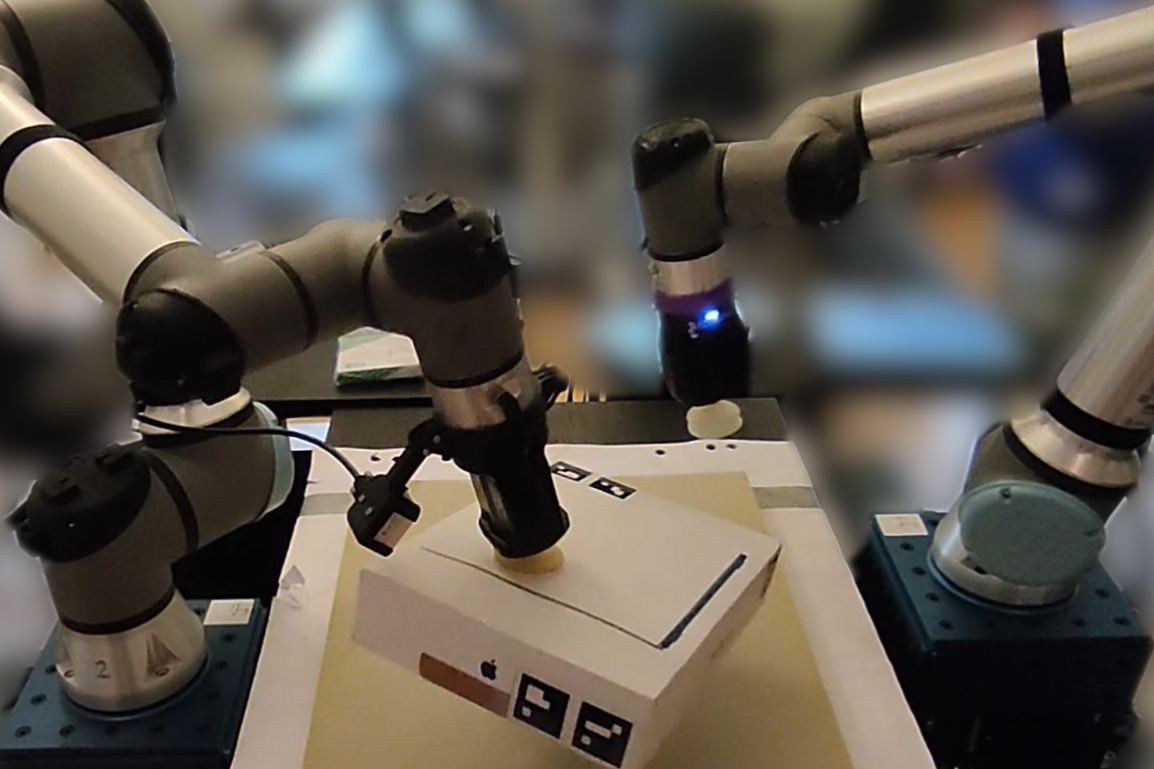
\includegraphics[width=0.9\linewidth]{images/fail_lift.png}}
    \subfigure[]{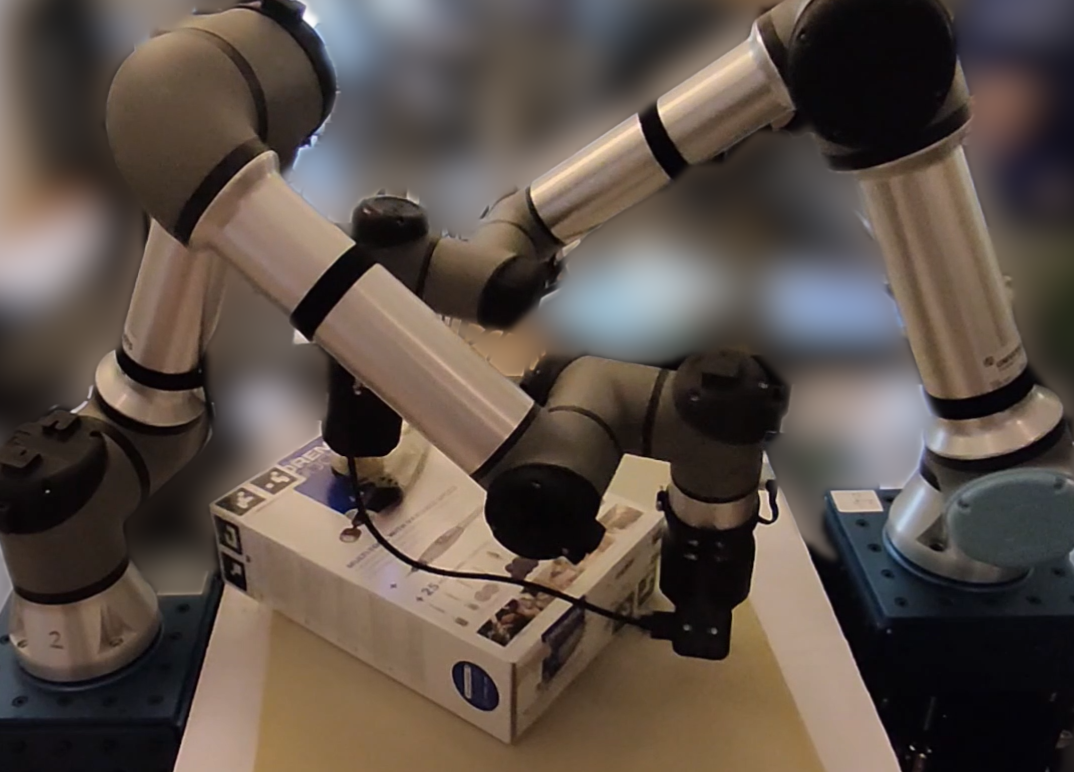
\includegraphics[width=0.9\linewidth]{images/rot_fail.png}}
    \caption{In (a), one single arm is lifting the box. In (b), one arm is rotating the box. Both policies achieve their sub-successes, respectively lifting and rotating, but do not grasp the box with both arms, leading to an unsuccessful episode.}
    \label{subsuccess-failure}
\end{figure}

Introducing visual information improved the policies' success rates, especially in the unseen scenario. 
From the results, it is clear that using only discrete information, for example, relying only on the box position and/or orientation, is not sufficient to achieve a policy that is general enough to work for every box. 
This also comes with the cost of a minimum four times longer training time.
Still, compared to other works, adding human interventions reduced the training time and was, most of the time, the key element to obtain a successful policy.

The worst performances on the unseen boxes can be related to the different sizes of the boxes, which have a big influence during the evaluation. For example, (8) and (9) struggled on the smaller boxes we used (ID 51 and 54), lowering the success rate of the whole task.
We didn't introduce more boxes at training time due to the constraints of the setup, but this should definitely be done in the future to enhance the policy's success rate.

As we mentioned in \cref{eval_details}, we couldn't train a policy using the RLPD algorithm for the motion task. As we saw with the other tasks, using this algorithm together with point cloud visual augmentation improves the performance of the policies. We expect a similar trend for the motion task, so it would be worth trying it out in future work.

While training a policy for the motion planning task, we found that using a similar pipeline as the one adopted for the previous tasks, i.e. initializing the replay buffer with 20 human-expert demonstrations, was not enough to obtain a successful policy.
In our opinion, the main difference with the first three tasks is that training online a policy to move an object to a point in a portion of space requires covering many more possible cases than the ones needed to train the other policies. 
The actions across the different episodes might not be similar and repetitive enough, therefore making the optimization problem harder. One could simplify the problem setup to always reach the same position in the space, but then we would need to retrain a new policy for every possible position in the space.

Therefore, we considered three solutions to fix this problem. First, as in \cite{luo2024precisedexterousroboticmanipulation} and \cite{nair2018overcomingexplorationreinforcementlearning}, we introduced two replay buffers. One is filled with demonstrations, and one with the online experience of the robots.  
During training, we equally sampled the data from both replay buffers.
In this way, we keep sampling and improving our policies using half of the data from the human-expert demonstrations recorded. 
Then, we trained two different policies. One in which we simply recorded more demonstrations, and another in which we kept the same number of demonstrations but introduced RRL as described in \cref{rrl} to act as a feedforward compensation term and help the policy to perform the required task. 

As reported in \cref{motion_sac_comparison}, when evaluating the performance on box 50, both success rates grow with respect to the performance of the policy simply initialized with 20 demonstrations, respectively by $37\%$ and $67\%$. Additionally, the motion sub-success improved respectively by $40\%$ and $67\%$. We did not study how the number of initial demonstrations influences the performance, and this number was picked considering the time required to record them.

\begin{table}[t]
    \centering
    \scriptsize
    \caption{Policy evaluation of the motion task. Results on box 50. 30 episodes are performed for every policy. The first policy is considered the baseline for the other two.}
    \renewcommand{\arraystretch}{1.5}
    \begin{tabular}{c|c|c|c|c}
        \toprule \textit{\textbf{Task}} & \textit{\textbf{Policy}} & \textit{\textbf{Success Rate [\%]}} & \textit{\textbf{Motion Sub-Success [\%]}} & \textit{\textbf{Demos}}\\
        \midrule & SAC & 3 & 13 & 20 \\
        Motion & SAC & 40 (\textcolor{green}{+37}) & 53 (\textcolor{green}{+40}) & 60 \\
         & SAC+RRL & \textbf{70} (\textcolor{green}{+67}) & \textbf{80} (\textcolor{green}{+67}) & 20 \\
        \bottomrule
    \end{tabular}
    \label{motion_sac_comparison}
\end{table}
\begin{table}[t]
    \centering
    \caption{Policy evaluation of the motion task. Trained with SAC using 60 human-expert demonstrations, but with different rewards and observations. For every policy, 30 runs are performed.}
    \renewcommand{\arraystretch}{1.5}
    \begin{tabular}{c|c|cc|cc}
        \toprule \textit{\textbf{Task}} & \textit{\textbf{Policy}} & \multicolumn{2}{c|}{\textit{\textbf{Success Rate [\%]}}} & \multicolumn{2}{c}{\textit{\textbf{Motion Sub-Success [\%]}}}\\
        & & \textit{Seen} & \textit{Unseen} & \textit{Seen} & \textit{Unseen}\\
        \midrule Motion & SAC & 40 & \textbf{30} & 53 & \textbf{47} \\
         & SAC & \textbf{67} & 11 & \textbf{70} & 13 \\
        \bottomrule
    \end{tabular}
    \label{sac_60demos_comparision}
\end{table}
\begin{table}[t]
    \centering
    \caption{Policy evaluation of the motion task. Trained with SAC using 60 human-expert demonstrations and evaluated at different checkpoints on box 50. For every policy, 30 runs are performed. The first policy is considered the baseline for the other two.}
    \renewcommand{\arraystretch}{1.5}
    \begin{tabular}{c|c|c|c}
        \toprule \textit{\textbf{Task}} & \textit{\textbf{Policy}} & \textit{\textbf{Checkpoint}} & \textit{\textbf{Success Rate [\%]}}\\
        \midrule  & SAC & 15000 & \textbf{67}\\
        Motion & SAC & 20000 & 33 (\textcolor{red}{-34})\\
        & SAC & 50000 & 30 (\textcolor{red}{-37})\\
        \bottomrule
    \end{tabular}
    \label{sac_rrl_comparision}
\end{table}

We performed several training runs to come up with a policy for the motion task, changing reward functions, weights, observations, or using the different techniques we mentioned in the previous paragraphs and sections.
Therefore, we obtained different policies using different solutions.
As reported in \cref{sac_60demos_comparision}, many policies performed slightly better than the one we reported in \cref{results}, but had a lower success rate on the unseen boxes. As our goal is to find a policy that effectively manipulates the widest and diverse set of boxes, we picked as a decision criterion that the better policies are those that achieve higher success rates on the unseen boxes.
Additionally, when running the evaluations, we noticed that different checkpoints of the network from the same training round have very different performances, as reported in \cref{sac_rrl_comparision}. Due to time constraints, we did not study this phenomenon extensively, but we mentioned it as the results of the policies and the related considerations at different checkpoints differ considerably. This made the whole evaluation more challenging and time-consuming. 

\section{CONCLUSIONS}

To the best of our knowledge, our approach is the first to train a reinforcement learning policy for a dual-arm system actuated with suction cups, using point cloud inputs, integrating HER and RRL while relying only on real-world data. In this work, we exploited the capabilities of this setup in performing learning-based object manipulation tasks, comparing the results with behavior tree baselines.

In future work, we want to explore other techniques to train robust policies while keeping short training times. 
Online reinforcement learning policies require much less data than policies trained in simulation. This makes training more challenging when the goal of the task and, therefore, the actions are not repetitive and change across different episodes.
Strategies to increase the sampling efficiency are needed in these cases. 

Increasing the number of initial demonstrations showed a possible way to enhance performances, but at a non-negligible cost of time. For example, recording 60 successful motion planning demonstrations took around 20 minutes, thanks to the fact that HER was used to recompute unsuccessful trajectories.

One possible solution would be to transform the observation reference frames. For example, representing all the observations with respect to the reference frame of the box or with respect to the goal position. This solution was not implemented because the noise coming from the pose estimation could have ruined the performance. Additionally, to the best of our knowledge, the literature related to this topic is scarce.

As mentioned in \cref{section-results}, introducing more boxes at training time would also be beneficial for the policies and better generalize the performances in unseen scenarios.

\addtolength{\textheight}{-1cm}   % This command serves to balance the column lengths
                                  % on the last page of the document manually. It shortens
                                  % the textheight of the last page by a suitable amount.
                                  % This command does not take effect until the next page
                                  % so it should come on the page before the last. Make
                                  % sure that you do not shorten the textheight too much.
                                  % default: 12cm

%%%%%%%%%%%%%%%%%%%%%%%%%%%%%%%%%%%%%%%%%%%%%%%%%%%%%%%%%%%%%%%%%%%%%%%%%%%%%%%%

\section*{ACKNOWLEDGMENT}

The authors thank Flink Robotics for practical and intellectual support.

%%%%%%%%%%%%%%%%%%%%%%%%%%%%%%%%%%%%%%%%%%%%%%%%%%%%%%%%%%%%%%%%%%%%%%%%%%%%%%%%

\printbibliography

%%%%%%%%%%%%%%%%%%%%%%%%%%%%%%%%%%%%%%%%%%%%%%%%%%%%%%%%%%%%%%%%%%%%%%%%%%%%%%%%


%%%%%%%%%%%%%%%%%%%%%%%%%%%%%%%%%%%%%%%%%%%%%%%%%%%%%%%%%%%%%%%%%%%%%%%%%%%%%%%%
\section*{APPENDIX}\label{appendix}

\subsection{Observations}
% rewards and observations
\begin{table}[H]
    \centering
    \renewcommand{\arraystretch}{1.5}
    \caption{Observations used during training and their corresponding scaling factors. The same values were used across all the tasks. Every task uses a different set of observations.}
    \begin{tabular}{c|c}
    \toprule \textit{\textbf{Observations}} & \textit{\textbf{Scaling factor}}\\
    \midrule tcp\_pos & 100 \\
    tcp\_orient & 10 \\
    tcp\_vel\_pos & 100\\
    tcp\_vel\_orient & 10\\
    gripper\_state & 1\\
    tcp\_force & 1\\
    tcp\_torque & 10\\
    tcp\_pos\_diff & 100\\
    joint\_position & 1\\
    action & 1\\
    goal\_box\_position & 10\\
    box\_position & 10\\
    box\_orientation & 10\\
    goal\_position & 10\\
    \bottomrule
    \end{tabular}
    \label{scaling_factors}
\end{table}

\subsection{Lift}

% rewards and observations
\begin{table}[H]
    \centering
    \caption{Observations used for the training of the lift task.}
    \renewcommand{\arraystretch}{1.5}
    \begin{tabular}{c|c}
    \toprule \textit{\textbf{Observations}} & \textit{\textbf{Dimension}}\\
    \midrule tcp\_pose & 14 \\
    tcp\_vel & 12 \\
    gripper\_state & 4 \\
    tcp\_force & 6\\
    tcp\_torque & 6\\
    tcp\_pos\_diff & 3\\
    joint\_position & 12\\
    action & 14 \\
    \bottomrule
    \end{tabular}
    \label{lift_obs}
\end{table}

\begin{table}[H]
    \centering
    \caption{Rewards and costs used for the training of the lift task (SAC).}
    \renewcommand{\arraystretch}{1.5}
    %\scriptsize
    \begin{tabular}{c|c}
    \toprule \textbf{\textit{Reward}} & \textbf{\textit{Formula}}\\
    \midrule Action & $-0.1\cdot || a_{t} ||^2_2$\\
    Speed & $-0.1\cdot || a_t -  a_{t-1}||^2_2$\\
    Step & -0.1\\
    Grasping & $1.5\cdot \text{bool}(grasped) $\\
    Suction & $-1.5\cdot \text{bool}(not\_grasped)$\\
    Orientation & $-25\cdot \text{relu}(1.995 - ||\Delta\phi_{1}||^2_2 - ||\Delta\phi_{2}||^2_2)$\\
    Position & $-10\cdot \sum_i |\Delta p_{i} - \text{sgn}(\Delta p_{i})* 0.05| $\\
    Early end & -10\\
    Success & $100\cdot [\text{bool}(grasped)\land (p>p_{start}+ 0.05)]$\\
    \bottomrule
    \end{tabular}
    \label{lift_rew_sac}
\end{table}

\begin{table}[H]
    \centering
    \caption{Rewards and costs for the training of the lift task (RLPD).}
    \renewcommand{\arraystretch}{1.5}
    %\scriptsize
    \begin{tabular}{c|c}
    \toprule \textbf{\textit{Reward}} & \textbf{\textit{Formula}}\\
    \midrule Action & $-0.1\cdot || a_{t} ||^2_2$\\
    Speed & $|| a_t - a_{t-1}||^2_2$ \\
    Step & -0.1\\
    Grasping & $1\cdot\text{bool}(grasped) $\\
    Suction & $1\cdot\text{bool}(not\_grasped) $ \\
    Orientation & $-10\cdot \text{relu}(1.995 - ||\Delta\phi_{1}||^2_2 - ||\Delta\phi_{2}||^2_2)$ \\
    Position & $-10\cdot \sum_i |\Delta p_{i} - \text{sgn}(\Delta p_{i})* 0.05| $\\
    Distance & $-0.5\cdot \frac{1}{||p_{ee_1} - p_{ee_2}||^2_2}$\\
    Grasping & $15\cdot \text{bool}(grasped) * p_z$\\
    Early end & -150\\
    Success & $200\cdot [\text{bool}(grasped)\land p >p_{start}+ 0.05]$ \\
    \bottomrule
    \end{tabular}
    \label{lift_rew_voxnet}
\end{table}

\subsection{Reorientation}

\begin{table}[H]
    \centering
    \caption{Observations used for the training of the rotation task.}
    \renewcommand{\arraystretch}{1.5}
    \begin{tabular}{c|c}
    \toprule \textit{\textbf{Observations}} & \textit{\textbf{Dimension}} \\
    \midrule tcp\_pose & 14\\
    tcp\_vel & 12 \\
    gripper\_state & 4 \\
    tcp\_force & 6 \\
    tcp\_torque & 6 \\
    tcp\_pos\_diff & 3 \\
    joint\_position & 12 \\
    action & 14 \\
    box\_orientation & 3 \\
    \bottomrule
    \end{tabular}
    \label{rot_obs}
\end{table}

\begin{table}[H]
    \centering
    \caption{Rewards and costs used for the training of the rotation task (SAC).}
    \renewcommand{\arraystretch}{1.5}
    %\scriptsize
    \begin{tabular}{c|c}
    \toprule \textbf{\textit{Reward}} & \textbf{\textit{Formula}}\\
    \midrule Action & $-0.1\cdot || a_{t} ||^2_2$\\
    Speed  & $-0.1\cdot || a_t - a_{t-1}||^2_2$\\
    Step & -0.1\\
    Grasping & $0.5\cdot \text{bool}(grasped) $\\
    Suction & $-0.5\cdot \text{bool}(not\_grasped) $\\
    Orientation & $-10\cdot \text{relu}(1.995 - ||\Delta\phi_{1}||^2_2 - ||\Delta\phi_{2}||^2_2)$\\
    Position & \makecell{$-15\cdot [\sum_i\text{bool}(grasped)|\Delta p_{i} - 0.35\text{sgn}(\Delta p_{i})|+$ \\ $\sum_i \text{bool}(not\_grasped)|\Delta p_{i} - 0.05\text{sgn}(\Delta p_{i})|]$}\\
    Rotation & $20\cdot min(max(\phi_{box_t} - \phi_{box_{t-1}}, 0.015), 0.3)$\\
    Early end & -10 \\
    Success & $200\cdot [\text{bool}(grasped)\land (|\Delta\Phi-$\SI{40}{\degree}$|)<$\SI{5}{\degree}$]$ \\
    \bottomrule
    \end{tabular}
    \label{rot_sac_rew}
\end{table}

\begin{table}[H]
    \centering
    \caption{Rewards and costs used for the training of the rotation task (RLPD).}
    \renewcommand{\arraystretch}{1.5}
    %\scriptsize
    \begin{tabular}{c|c}
    \toprule \textbf{\textit{Reward}} & \textbf{\textit{Formula}}\\
    \midrule Action & $-0.1\cdot || a_{t} ||^2_2$\\
    Speed  & $-0.1\cdot || a_t - a_{t-1}||^2_2$\\
    Step & -0.1\\
    Grasping & $0.5\cdot \text{bool}(grasped) $\\
    Suction & $-0.5\cdot \text{bool}(not\_grasped) $\\
    Orientation & $-30\cdot \text{relu}(1.995 - ||\Delta\phi_{1}||^2_2 - ||\Delta\phi_{2}||^2_2)$\\
    Position & \makecell{$-15\cdot [\sum_i\text{bool}(grasped)|\Delta p_{i} - 0.35\text{sgn}(\Delta p_{i})|+$ \\ $\sum_i \text{bool}(not\_grasped)|\Delta p_{i} - 0.05\text{sgn}(\Delta p_{i})|]$}\\
    Distance & $-0.1\cdot \frac{1}{||p_{ee_1} - p_{ee_2}||^2_2}$\\
    Rotation & $20\cdot min(max(\phi_{box_t} - \phi_{box_{t-1}}, 0.015), 0.3)$\\
    Early end & -150 \\
    Success & $200\cdot [\text{bool}(grasped)\land (|\Delta\Phi-$\SI{40}{\degree}$|)<$\SI{5}{\degree}$]$ \\
    \bottomrule
    \end{tabular}
    \label{rot_drq_rew}
\end{table}

\subsection{Lift+rotation}

\begin{table}[H]
    \centering
    \caption{Observations used for the training of the lift \& rotation task.}
    \renewcommand{\arraystretch}{1.5}
    \begin{tabular}{c|c}
    \toprule \textit{\textbf{Observations}} & \textit{\textbf{Dimension}} \\
    \midrule tcp\_pose & 14 \\
    tcp\_vel & 12 \\
    gripper\_state & 4 \\
    tcp\_pos\_diff & 3 \\
    joint\_position & 12 \\
    action & 14 \\
    box\_position & 3 \\
    box\_orientation & 3 \\
    \bottomrule
    \end{tabular}
    \label{inair_obs}
\end{table}

\begin{table}[H]
    \centering
    \caption{Rewards and costs used for the training of the lift \& rotation task (SAC).}
    \renewcommand{\arraystretch}{1.5}
    %\scriptsize
    \begin{tabular}{c|c}
    \toprule \textbf{\textit{Reward}} & \textbf{\textit{Formula}}\\
    \midrule Action & $-0.2\cdot || a_{t} ||^2_2$\\
    Speed & $-0.2\cdot || a_t - a_{t-1}||^2_2$\\
    Step & -0.2\\
    Grasping & $0.5\cdot \text{bool}(grasped)$\\
    Suction & $-0.5\cdot \text{bool}(not\_grasped)$\\
    Position & $-0.5\cdot \text{bool}(p_t-p_0<0.05)$\\
    Rotation & $40\cdot min(max(\phi_{box_t} - \phi_{box_{t-1}}, 0.015), 0.3)$\\
    Early end & -150\\
    Success & $200\cdot [\text{bool}(grasped)\land (|\Delta\Phi-$\SI{40}{\degree}$|)<$\SI{5}{\degree}$]$ \\
    \bottomrule
    \end{tabular}
    \label{inair_sac_rew}
\end{table}

\begin{table}[H]
    \centering
    \caption{Rewards and costs used for the training of the lift \& rotation task (RLPD).}
    \renewcommand{\arraystretch}{1.5}
    %\scriptsize
    \begin{tabular}{c|c}
    \toprule \textbf{\textit{Reward}} & \textbf{\textit{Formula}}\\
    \midrule Action & $-0.2\cdot || a_{t} ||^2_2$\\
    Speed & $-0.2\cdot || a_t - a_{t-1}||^2_2$\\
    Step & -0.2\\
    Grasping & $0.5\cdot \text{bool}(grasped)$\\
    Suction & $-0.5\cdot \text{bool}(not\_grasped)$\\
    Position & $-0.5\cdot \text{bool}(p_t-p_0<0.05)$\\
    Rotation & $40\cdot min(max(\phi_{box_t} - \phi_{box_{t-1}}, 0.015), 0.3)$\\
    Distance & $-0.05\cdot \frac{1}{||p_{ee_1} - p_{ee_2}||^2_2}$\\
    Early end & -150\\
    Success & $200\cdot [\text{bool}(grasped)\land (|\Delta\Phi-$\SI{40}{\degree}$|)<$\SI{5}{\degree}$]$ \\
    \bottomrule
    \end{tabular}
    \label{inair_drq_rew}
\end{table}

\subsection{Motion}

\begin{table}[H]
    \centering
    \caption{Observations used for the training of the motion task. Policy (11) used the following set of observations.}
    \renewcommand{\arraystretch}{1.5}
    \begin{tabular}{c|c}
    \toprule \textit{\textbf{Observations}} & \textit{\textbf{Dimension}} \\
    \midrule tcp\_pose & 14 \\
    tcp\_vel & 12 \\
    gripper\_state & 4 \\
    tcp\_pos\_diff & 3 \\
    joint\_position & 12 \\
    action & 14 \\
    goal\_box\_position & 3 \\
    box\_position & 3 \\
    goal\_position & 3 \\
    \bottomrule
    \end{tabular}
    \label{motion_obs_sac}
\end{table}

\begin{table}[H]
    \centering
    \caption{Rewards and costs used for the training of the motion task (SAC). Note that the \textit{Goal distance} reward is computed as written in \cref{normalized_goal_box}.}
    \renewcommand{\arraystretch}{1.5}
    %\scriptsize
    \begin{tabular}{c|c}
    \toprule \textbf{\textit{Reward}} & \textbf{\textit{Formula}}\\
    \midrule Action & $-0.1\cdot || a_{t} ||^2_2$\\
    Speed & $-0.1\cdot ||a_t - a_{t-1}||^2_2$\\
    Step & -0.1\\
    Grasping & $0.3\cdot \text{bool}(grasped) $\\
    Suction & $-0.5\cdot \text{bool}(not\_grasped)$\\
    Orientation & $-4\cdot \text{relu}(1.995 - ||\Delta\phi_{1}||^2_2 - ||\Delta\phi_{2}||^2_2)$\\
    Position & $-4\cdot ||goal\_box\_dist||^2_2$\\
    Goal distance & $60\cdot norm(p^{box}_t, p^{box}_{t-1})$\\    
    Early end & -150\\
    Success & $200\cdot [\text{bool}(grasped)\land (||goal\_box\_dist||^2_2 <0.05)]$\\
    \bottomrule
    \end{tabular}
    \label{motion_rew_sac}
\end{table}

\begin{table}[H]
    \centering
    \caption{Observations used for the training of the motion task. Policy (12) used the following set of observations.}
    \renewcommand{\arraystretch}{1.5}
    \begin{tabular}{c|c}
    \toprule \textit{\textbf{Observations}} & \textit{\textbf{Dimension}} \\
    \midrule tcp\_pose & 14 \\
    tcp\_vel & 12 \\
    gripper\_state & 4 \\
    action & 14 \\
    goal\_box\_position & 3 \\
    box\_position & 3 \\
    goal\_position & 3 \\
    \bottomrule
    \end{tabular}
    \label{motion_obs_sac_rrl}
\end{table}

\begin{table}[H]
    \centering
    \caption{Rewards and costs used for the training of the motion task (SAC+RRL). Note that the \textit{Goal distance} reward is computed as written in \cref{normalized_goal_box}.}
    \renewcommand{\arraystretch}{1.5}
    %\scriptsize
    \begin{tabular}{c|c}
    \toprule \textbf{\textit{Reward}} & \textbf{\textit{Formula}}\\
    \midrule Action & $-0.3\cdot || a_{t} ||^2_2$\\
    Speed & $-0.3\cdot ||a_t - a_{t-1}||^2_2$\\
    Step & -0.2\\
    Grasping & $2\cdot \text{bool}(grasped) $\\
    Suction & $-1\cdot \text{bool}(not\_grasped)$\\
    Orientation & $-10\cdot \text{relu}(1.995 - ||\Delta\phi_{1}||^2_2 - ||\Delta\phi_{2}||^2_2)$\\
    Position & $-10\cdot ||goal\_box\_dist||^2_2$\\
    Goal distance & $80\cdot norm(p^{box}_t, p^{box}_{t-1})$\\
    Distance & $-0.5\cdot \frac{1}{||p_{ee_1} - p_{ee_2}||^2_2}$\\    Early end & -150\\
    Success & $200\cdot [\text{bool}(grasped)\land (||goal\_box\_dist||^2_2 <0.05)]$\\
    \bottomrule
    \end{tabular}
    \label{motion_rew_sac_rrl}
\end{table}

\subsection{Complete evaluation}

\begin{table*}[t]
    \centering
    \caption{Evaluation of the lift task. 30 episodes are performed for every policy.}
    \renewcommand{\arraystretch}{1.5}
    \begin{tabular}{c|c|cc|cc|cc|cc}
        \toprule \textbf{\textit{Task}} & \textbf{\textit{Policy}} & \multicolumn{2}{c|}{\textit{\textbf{Success Rate [\%]}}} & \multicolumn{2}{c|}{\textit{\textbf{Grasp Sub-success [\%]}}} & \multicolumn{2}{c|}{\textit{\textbf{Lift Sub-success [\%]}}} & \multicolumn{2}{c}{\textit{\textbf{Time [s]}}}\\
        & & \textit{Seen} & \textit{Unseen} & \textit{Seen} & \textit{Unseen} & \textit{Seen} & \textit{Unseen} & \textit{Seen} & \textit{Unseen} \\
        \midrule & BT & 77 & \textbf{66} & \textbf{100} & 99 & 77 & 66 & \textbf{5.57} $\pm$ 2.54 & \textbf{6.86} $\pm$ 2.20 \\
        Lift & SAC & 70 & 28 & \textbf{100} & 95 & 93 & 66 & 9.07 $\pm$ 5.14 & 11.79 $\pm$ 3.58 \\
         & RLPD & \textbf{100} & 55 & \textbf{100} & \textbf{100} & \textbf{100} & \textbf{95} & 11.49 $\pm$ 3.00 & 12.88 $\pm$ 6.20 \\
        \bottomrule
    \end{tabular}
    \label{lift_eval}
\end{table*}

\begin{table*}[t]
    \centering
    \caption{Evaluation of the rotation task. 30 episodes are performed for every policy.}
    \renewcommand{\arraystretch}{1.5}
    \begin{tabular}{c|c|cc|cc|cc|cc}
        \toprule \textit{\textbf{Task}} & \textit{\textbf{Policy}} & \multicolumn{2}{c|}{\textit{\textbf{Success Rate [\%]}}} & \multicolumn{2}{c|}{\textit{\textbf{Grasp Sub-success [\%]}}} & \multicolumn{2}{c|}{\textit{\textbf{Rotation Sub-success [\%]}}} & \multicolumn{2}{c}{\textit{\textbf{Time [s]}}} \\
        & & \textit{Seen} & \textit{Unseen} & \textit{Seen} & \textit{Unseen} & \textit{Seen} & \textit{Unseen} & \textit{Seen} & \textit{Unseen} \\
        \midrule
        & BT & 60 & 62 & \textbf{100} & 98 & 60 & 62 & $7.80 \pm 1.92$ & \textbf{6.95} $\pm 1.91$ \\
        Rotation & SAC & \textbf{100} & 75 & \textbf{100} & \textbf{100} & \textbf{100} & \textbf{98} & $8.94 \pm 0.59$ & $10.99 \pm 3.74$ \\
        & RLPD & \textbf{100} & \textbf{90} & \textbf{100} & \textbf{100} & \textbf{100} & 95 & \textbf{5.70} $\pm$ 0.38 & $8.52 \pm 5.92$ \\
        \bottomrule
    \end{tabular}
    \label{rot_eval}
\end{table*}


\begin{table*}[t]
    \centering
    \caption{Evaluation of the lift \& rotation task. 30 episodes are performed for every policy.}
    \renewcommand{\arraystretch}{1.5}
    \begin{tabular}{c|c|cc|cc|cc|cc|cc}
        \toprule \textit{\textbf{Task}} & \textit{\textbf{Policy}} & \multicolumn{2}{c|}{\textit{\textbf{Success Rate [\%]}}} & \multicolumn{2}{c|}{\textit{\textbf{Grasp Sub-success [\%]}}} & \multicolumn{2}{c|}{\textit{\textbf{Lift Sub-success [\%]}}} & \multicolumn{2}{c|}{\textit{\textbf{Rot Sub-success [\%]}}} & \multicolumn{2}{c}{\textit{\textbf{Time [s]}}} \\
        & & \textit{Seen} & \textit{Unseen} & \textit{Seen} & \textit{Unseen} & \textit{Seen} & \textit{Unseen} & \textit{Seen} & \textit{Unseen} & \textit{Seen} & \textit{Unseen}\\
        \midrule 
        Lift & BT & 60 & 61 & \textbf{100} & \textbf{97} & 77 & 77 & 63 & 61 & 8.71 $\pm$ 1.31 & \textbf{8.38} $\pm$ 1.66 \\
        \& & SAC & \textbf{97} & 28 & \textbf{100} & \textbf{97} & 97 & 55 & 97 & 50 & 7.71 $\pm$ 2.24 & 12.15 $\pm$ 3.86 \\
        Rotation & RLPD & \textbf{97} & \textbf{69} & \textbf{100} & 95 & \textbf{100} & \textbf{79} & \textbf{100} & \textbf{86} & \textbf{4.85} $\pm$ 2.25 & 8.49 $\pm$ 3.96 \\
        \bottomrule
    \end{tabular}
    \label{inair_eval}
\end{table*}


\begin{table*}[t]
    \centering
    \scriptsize
    \caption{Evaluation of the motion task. 30 episodes are performed for every policy.}
    \renewcommand{\arraystretch}{1.5}
    \begin{tabular}{c|c|cc|cc|cc|cc|cc}
        \toprule \textit{\textbf{Task}} & \textit{\textbf{Policy}} & \multicolumn{2}{c|}{\textit{\textbf{Success Rate [\%]}}} & \multicolumn{2}{c|}{\textit{\textbf{Grasp Sub-success [\%]}}} & \multicolumn{2}{c|}{\textit{\textbf{Motion Sub-success [\%]}}} & \multicolumn{2}{c|}{\textit{\textbf{Distance from goal [m]}}} & \multicolumn{2}{c}{\textit{\textbf{Time [s]}}} \\
        & & \textit{Seen} & \textit{Unseen} & \textit{Seen} & \textit{Unseen} & \textit{Seen} & \textit{Unseen} & \textit{Seen} & \textit{Unseen} & \textit{Seen} & \textit{Unseen}\\
        \midrule & BT & 67 & \textbf{55} & \textbf{100} & \textbf{100} & 67 & 55 & 0.110 & 0.120 & \textbf{8.80} $\pm$ 1.23 & \textbf{9.06} $\pm$ 1.03 \\
        Motion & SAC & 40 & 30 & \textbf{100} & 98 & 53 & 47 & 0.072 & 0.089 & 11.62 $\pm$ 3.20 & 12.93 $\pm$ 4.25 \\
         & SAC + RRL & \textbf{70} & 37 & \textbf{100} & \textbf{100} & \textbf{80} & \textbf{56} & \textbf{0.063} & \textbf{0.083} & 11.67 $\pm$ 4.61 & 14.19 $\pm$ 3.03 \\
        \bottomrule
    \end{tabular}
    \label{motion_eval}
\end{table*}


\end{document}
